\documentclass[11pt,a4paper]{report}
\usepackage{isabelle,isabellesym,pdfsetup}
\usepackage{latexsym,verbatim,graphicx,../iman,extra,comment}

\usepackage{ttbox}
\newcommand\ttbreak{\vskip-10pt\pagebreak[0]}
\newcommand\Out[1]{\texttt{\textsl{#1}}}   %% for output from terminal sessions

%\newtheorem{theorem}{Theorem}[section]
\newtheorem{Exercise}{Exercise}[section]
\newenvironment{exercise}{\begin{Exercise}\rm}{\end{Exercise}}
\newcommand{\ttlbr}{\texttt{[|}}
\newcommand{\ttrbr}{\texttt{|]}}
\newcommand{\ttor}{\texttt{|}}
\newcommand{\ttall}{\texttt{!}}
\newcommand{\ttuniquex}{\texttt{?!}}
\newcommand{\ttEXU}{\texttt{EX!}}
\newcommand{\ttAnd}{\texttt{!!}}

\newcommand{\isasymimp}{\isasymlongrightarrow}
\newcommand{\isasymImp}{\isasymLongrightarrow}
\newcommand{\isasymFun}{\isasymRightarrow}
\newcommand{\isasymuniqex}{\emph{$\exists!\,$}}

\newenvironment{isabellepar}%
{\par\medskip\noindent\begin{isabelle}}{\end{isabelle}\medskip\par\noindent}

\renewenvironment{isamarkuptxt}{\begin{isamarkuptext}}{\end{isamarkuptext}}

%%% to index derived rls:  ^\([a-zA-Z0-9][a-zA-Z0-9_]*\)        \\tdx{\1}  
%%% to index rulenames:   ^ *(\([a-zA-Z0-9][a-zA-Z0-9_]*\),     \\tdx{\1}  
%%% to index constants:   \\tt \([a-zA-Z0-9][a-zA-Z0-9_]*\)     \\cdx{\1}  
%%% to deverbify:         \\verb|\([^|]*\)|     \\ttindex{\1}  
%% run    ../sedindex logics    to prepare index file

\makeindex
\newcommand{\indexboldpos}[2]{#1\indexbold{#2@#1}}
\newcommand{\ttindexboldpos}[2]{\texttt{#1}\indexbold{#2@\texttt{#1}}}
\newcommand{\isaindexbold}[1]{\isa{#1}\index{*#1|bold}}
\newcommand{\isaindex}[1]{\isa{#1}\index{*#1}}

\underscoreoff

\setcounter{secnumdepth}{2} \setcounter{tocdepth}{2}  %% {secnumdepth}{2}???

\pagestyle{headings}
%\sloppy
%\binperiod     %%%treat . like a binary operator

\begin{document}
\title{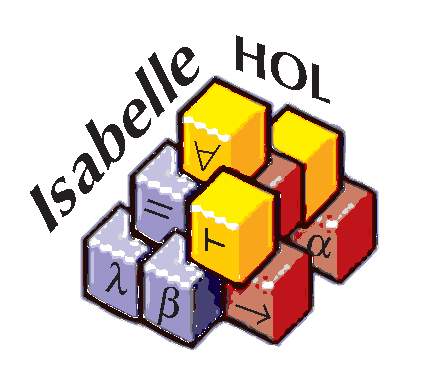
\includegraphics[scale=.8]{isabelle_hol}
       \\ \vspace{0.5cm} The Tutorial
       \\ --- DRAFT ---}
\author{Tobias Nipkow\\
Technische Universit\"at M\"unchen \\
Institut f\"ur Informatik \\
\url{http://www.in.tum.de/~nipkow/}}
\maketitle

\pagenumbering{roman}
\tableofcontents

\subsubsection*{Acknowledgements}
This tutorial owes a lot to the constant discussions with and the valuable
feedback from Larry Paulson and the Isabelle group at Munich: Olaf M\"uller,
Wolfgang Naraschewski, David von Oheimb, Leonor Prensa Nieto, Cornelia Pusch
and Markus Wenzel. Stefan Berghofer and Stephan Merz were also kind enough to
read and comment on a draft version.
\clearfirst

\chapter{The Basics}

\section{Introduction}

This book is a tutorial on how to use the theorem prover Isabelle/HOL as a
specification and verification system. Isabelle is a generic system for
implementing logical formalisms, and Isabelle/HOL is the specialization
of Isabelle for HOL, which abbreviates Higher-Order Logic. We introduce
HOL step by step following the equation
\[ \mbox{HOL} = \mbox{Functional Programming} + \mbox{Logic}. \]
We do not assume that you are familiar with mathematical logic. 
However, we do assume that
you are used to logical and set theoretic notation, as covered
in a good discrete mathematics course~\cite{Rosen-DMA}, and
that you are familiar with the basic concepts of functional
programming~\cite{Bird-Haskell,Hudak-Haskell,paulson-ml2,Thompson-Haskell}.
Although this tutorial initially concentrates on functional programming, do
not be misled: HOL can express most mathematical concepts, and functional
programming is just one particularly simple and ubiquitous instance.

Isabelle~\cite{paulson-isa-book} is implemented in ML~\cite{SML}.  This has
influenced some of Isabelle/HOL's concrete syntax but is otherwise irrelevant
for us: this tutorial is based on
Isabelle/Isar~\cite{isabelle-isar-ref}, an extension of Isabelle which hides
the implementation language almost completely.  Thus the full name of the
system should be Isabelle/Isar/HOL, but that is a bit of a mouthful.

There are other implementations of HOL, in particular the one by Mike Gordon
\index{Gordon, Mike}%
\emph{et al.}, which is usually referred to as ``the HOL system''
\cite{mgordon-hol}. For us, HOL refers to the logical system, and sometimes
its incarnation Isabelle/HOL\@.

A tutorial is by definition incomplete.  Currently the tutorial only
introduces the rudiments of Isar's proof language. To fully exploit the power
of Isar, in particular the ability to write readable and structured proofs,
you need to consult the Isabelle/Isar Reference
Manual~\cite{isabelle-isar-ref} and Wenzel's PhD thesis~\cite{Wenzel-PhD}
which discusses many proof patterns. If you want to use Isabelle's ML level
directly (for example for writing your own proof procedures) see the Isabelle
Reference Manual~\cite{isabelle-ref}; for details relating to HOL see the
Isabelle/HOL manual~\cite{isabelle-HOL}. All manuals have a comprehensive
index.

\section{Theories}
\label{sec:Basic:Theories}

\index{theories|(}%
Working with Isabelle means creating theories. Roughly speaking, a
\textbf{theory} is a named collection of types, functions, and theorems,
much like a module in a programming language or a specification in a
specification language. In fact, theories in HOL can be either. The general
format of a theory \texttt{T} is
\begin{ttbox}
theory T
imports B\(@1\) \(\ldots\) B\(@n\)
begin
{\rmfamily\textit{declarations, definitions, and proofs}}
end
\end{ttbox}\cmmdx{theory}\cmmdx{imports}
where \texttt{B}$@1$ \dots\ \texttt{B}$@n$ are the names of existing
theories that \texttt{T} is based on and \textit{declarations,
    definitions, and proofs} represents the newly introduced concepts
(types, functions etc.) and proofs about them. The \texttt{B}$@i$ are the
direct \textbf{parent theories}\indexbold{parent theories} of~\texttt{T}\@.
Everything defined in the parent theories (and their parents, recursively) is
automatically visible. To avoid name clashes, identifiers can be
\textbf{qualified}\indexbold{identifiers!qualified}
by theory names as in \texttt{T.f} and~\texttt{B.f}. 
Each theory \texttt{T} must
reside in a \textbf{theory file}\index{theory files} named \texttt{T.thy}.

This tutorial is concerned with introducing you to the different linguistic
constructs that can fill the \textit{declarations, definitions, and
    proofs} above.  A complete grammar of the basic
constructs is found in the Isabelle/Isar Reference
Manual~\cite{isabelle-isar-ref}.

HOL's theory collection is available online at
\begin{center}\small
    \url{http://isabelle.in.tum.de/library/HOL/}
\end{center}
and is recommended browsing. Note that most of the theories 
are based on classical Isabelle without the Isar extension. This means that
they look slightly different than the theories in this tutorial, and that all
proofs are in separate ML files.

\begin{warn}
  HOL contains a theory \thydx{Main}, the union of all the basic
  predefined theories like arithmetic, lists, sets, etc.  
  Unless you know what you are doing, always include \isa{Main}
  as a direct or indirect parent of all your theories.
\end{warn}
There is also a growing Library~\cite{HOL-Library}\index{Library}
of useful theories that are not part of \isa{Main} but can be included
among the parents of a theory and will then be loaded automatically.%
\index{theories|)}


\section{Types, Terms and Formulae}
\label{sec:TypesTermsForms}

Embedded in a theory are the types, terms and formulae of HOL\@. HOL is a typed
logic whose type system resembles that of functional programming languages
like ML or Haskell. Thus there are
\index{types|(}
\begin{description}
\item[base types,] 
in particular \tydx{bool}, the type of truth values,
and \tydx{nat}, the type of natural numbers.
\item[type constructors,]\index{type constructors}
 in particular \tydx{list}, the type of
lists, and \tydx{set}, the type of sets. Type constructors are written
postfix, e.g.\ \isa{(nat)list} is the type of lists whose elements are
natural numbers. Parentheses around single arguments can be dropped (as in
\isa{nat list}), multiple arguments are separated by commas (as in
\isa{(bool,nat)ty}).
\item[function types,]\index{function types}
denoted by \isasymFun\indexbold{$IsaFun@\isasymFun}.
  In HOL \isasymFun\ represents \emph{total} functions only. As is customary,
  \isa{$\tau@1$ \isasymFun~$\tau@2$ \isasymFun~$\tau@3$} means
  \isa{$\tau@1$ \isasymFun~($\tau@2$ \isasymFun~$\tau@3$)}. Isabelle also
  supports the notation \isa{[$\tau@1,\dots,\tau@n$] \isasymFun~$\tau$}
  which abbreviates \isa{$\tau@1$ \isasymFun~$\cdots$ \isasymFun~$\tau@n$
    \isasymFun~$\tau$}.
\item[type variables,]\index{type variables}\index{variables!type}
  denoted by \ttindexboldpos{'a}{$Isatype}, \isa{'b} etc., just like in ML\@. They give rise
  to polymorphic types like \isa{'a \isasymFun~'a}, the type of the identity
  function.
\end{description}
\begin{warn}
  Types are extremely important because they prevent us from writing
  nonsense.  Isabelle insists that all terms and formulae must be well-typed
  and will print an error message if a type mismatch is encountered. To
  reduce the amount of explicit type information that needs to be provided by
  the user, Isabelle infers the type of all variables automatically (this is
  called \bfindex{type inference}) and keeps quiet about it. Occasionally
  this may lead to misunderstandings between you and the system. If anything
  strange happens, we recommend that you set the flag\index{flags}
  \isa{show_types}\index{*show_types (flag)}.  
  Isabelle will then display type information
  that is usually suppressed.  Simply type
\begin{ttbox}
ML "set show_types"
\end{ttbox}

\noindent
This can be reversed by \texttt{ML "reset show_types"}. Various other flags,
which we introduce as we go along, can be set and reset in the same manner.%
\index{flags!setting and resetting}
\end{warn}%
\index{types|)}


\index{terms|(}
\textbf{Terms} are formed as in functional programming by
applying functions to arguments. If \isa{f} is a function of type
\isa{$\tau@1$ \isasymFun~$\tau@2$} and \isa{t} is a term of type
$\tau@1$ then \isa{f~t} is a term of type $\tau@2$. HOL also supports
infix functions like \isa{+} and some basic constructs from functional
programming, such as conditional expressions:
\begin{description}
\item[\isa{if $b$ then $t@1$ else $t@2$}]\index{*if expressions}
Here $b$ is of type \isa{bool} and $t@1$ and $t@2$ are of the same type.
\item[\isa{let $x$ = $t$ in $u$}]\index{*let expressions}
is equivalent to $u$ where all free occurrences of $x$ have been replaced by
$t$. For example,
\isa{let x = 0 in x+x} is equivalent to \isa{0+0}. Multiple bindings are separated
by semicolons: \isa{let $x@1$ = $t@1$;\dots; $x@n$ = $t@n$ in $u$}.
\item[\isa{case $e$ of $c@1$ \isasymFun~$e@1$ |~\dots~| $c@n$ \isasymFun~$e@n$}]
\index{*case expressions}
evaluates to $e@i$ if $e$ is of the form $c@i$.
\end{description}

Terms may also contain
\isasymlambda-abstractions.\index{lambda@$\lambda$ expressions}
For example,
\isa{\isasymlambda{}x.~x+1} is the function that takes an argument \isa{x} and
returns \isa{x+1}. Instead of
\isa{\isasymlambda{}x.\isasymlambda{}y.\isasymlambda{}z.~$t$} we can write
\isa{\isasymlambda{}x~y~z.~$t$}.%
\index{terms|)}

\index{formulae|(}%
\textbf{Formulae} are terms of type \tydx{bool}.
There are the basic constants \cdx{True} and \cdx{False} and
the usual logical connectives (in decreasing order of priority):
\indexboldpos{\protect\isasymnot}{$HOL0not}, \indexboldpos{\protect\isasymand}{$HOL0and},
\indexboldpos{\protect\isasymor}{$HOL0or}, and \indexboldpos{\protect\isasymimp}{$HOL0imp},
all of which (except the unary \isasymnot) associate to the right. In
particular \isa{A \isasymimp~B \isasymimp~C} means \isa{A \isasymimp~(B
  \isasymimp~C)} and is thus logically equivalent to \isa{A \isasymand~B
  \isasymimp~C} (which is \isa{(A \isasymand~B) \isasymimp~C}).

Equality\index{equality} is available in the form of the infix function
\isa{=} of type \isa{'a \isasymFun~'a
  \isasymFun~bool}. Thus \isa{$t@1$ = $t@2$} is a formula provided $t@1$
and $t@2$ are terms of the same type. If $t@1$ and $t@2$ are of type
\isa{bool} then \isa{=} acts as \rmindex{if-and-only-if}.
The formula
\isa{$t@1$~\isasymnoteq~$t@2$} is merely an abbreviation for
\isa{\isasymnot($t@1$ = $t@2$)}.

Quantifiers\index{quantifiers} are written as
\isa{\isasymforall{}x.~$P$} and \isa{\isasymexists{}x.~$P$}. 
There is even
\isa{\isasymuniqex{}x.~$P$}, which
means that there exists exactly one \isa{x} that satisfies \isa{$P$}. 
Nested quantifications can be abbreviated:
\isa{\isasymforall{}x~y~z.~$P$} means
\isa{\isasymforall{}x.\isasymforall{}y.\isasymforall{}z.~$P$}.%
\index{formulae|)}

Despite type inference, it is sometimes necessary to attach explicit
\bfindex{type constraints} to a term.  The syntax is
\isa{$t$::$\tau$} as in \isa{x < (y::nat)}. Note that
\ttindexboldpos{::}{$Isatype} binds weakly and should therefore be enclosed
in parentheses.  For instance,
\isa{x < y::nat} is ill-typed because it is interpreted as
\isa{(x < y)::nat}.  Type constraints may be needed to disambiguate
expressions
involving overloaded functions such as~\isa{+}, 
\isa{*} and~\isa{<}.  Section~\ref{sec:overloading} 
discusses overloading, while Table~\ref{tab:overloading} presents the most
important overloaded function symbols.

In general, HOL's concrete \rmindex{syntax} tries to follow the conventions of
functional programming and mathematics.  Here are the main rules that you
should be familiar with to avoid certain syntactic traps:
\begin{itemize}
\item
Remember that \isa{f t u} means \isa{(f t) u} and not \isa{f(t u)}!
\item
Isabelle allows infix functions like \isa{+}. The prefix form of function
application binds more strongly than anything else and hence \isa{f~x + y}
means \isa{(f~x)~+~y} and not \isa{f(x+y)}.
\item Remember that in HOL if-and-only-if is expressed using equality.  But
  equality has a high priority, as befitting a relation, while if-and-only-if
  typically has the lowest priority.  Thus, \isa{\isasymnot~\isasymnot~P =
    P} means \isa{\isasymnot\isasymnot(P = P)} and not
  \isa{(\isasymnot\isasymnot P) = P}. When using \isa{=} to mean
  logical equivalence, enclose both operands in parentheses, as in \isa{(A
    \isasymand~B) = (B \isasymand~A)}.
\item
Constructs with an opening but without a closing delimiter bind very weakly
and should therefore be enclosed in parentheses if they appear in subterms, as
in \isa{(\isasymlambda{}x.~x) = f}.  This includes 
\isa{if},\index{*if expressions}
\isa{let},\index{*let expressions}
\isa{case},\index{*case expressions}
\isa{\isasymlambda}, and quantifiers.
\item
Never write \isa{\isasymlambda{}x.x} or \isa{\isasymforall{}x.x=x}
because \isa{x.x} is always taken as a single qualified identifier. Write
\isa{\isasymlambda{}x.~x} and \isa{\isasymforall{}x.~x=x} instead.
\item Identifiers\indexbold{identifiers} may contain the characters \isa{_} 
and~\isa{'}, except at the beginning.
\end{itemize}

For the sake of readability, we use the usual mathematical symbols throughout
the tutorial. Their \textsc{ascii}-equivalents are shown in table~\ref{tab:ascii} in
the appendix.

\begin{warn}
A particular
problem for novices can be the priority of operators. If you are unsure, use
additional parentheses. In those cases where Isabelle echoes your
input, you can see which parentheses are dropped --- they were superfluous. If
you are unsure how to interpret Isabelle's output because you don't know
where the (dropped) parentheses go, set the flag\index{flags}
\isa{show_brackets}\index{*show_brackets (flag)}:
\begin{ttbox}
ML "set show_brackets"; \(\dots\); ML "reset show_brackets";
\end{ttbox}
\end{warn}


\section{Variables}
\label{sec:variables}
\index{variables|(}

Isabelle distinguishes free and bound variables, as is customary. Bound
variables are automatically renamed to avoid clashes with free variables. In
addition, Isabelle has a third kind of variable, called a \textbf{schematic
  variable}\index{variables!schematic} or \textbf{unknown}\index{unknowns}, 
which must have a~\isa{?} as its first character.  
Logically, an unknown is a free variable. But it may be
instantiated by another term during the proof process. For example, the
mathematical theorem $x = x$ is represented in Isabelle as \isa{?x = ?x},
which means that Isabelle can instantiate it arbitrarily. This is in contrast
to ordinary variables, which remain fixed. The programming language Prolog
calls unknowns {\em logical\/} variables.

Most of the time you can and should ignore unknowns and work with ordinary
variables. Just don't be surprised that after you have finished the proof of
a theorem, Isabelle will turn your free variables into unknowns.  It
indicates that Isabelle will automatically instantiate those unknowns
suitably when the theorem is used in some other proof.
Note that for readability we often drop the \isa{?}s when displaying a theorem.
\begin{warn}
  For historical reasons, Isabelle accepts \isa{?} as an ASCII representation
  of the \(\exists\) symbol.  However, the \isa{?} character must then be followed
  by a space, as in \isa{?~x. f(x) = 0}.  Otherwise, \isa{?x} is
  interpreted as a schematic variable.  The preferred ASCII representation of
  the \(\exists\) symbol is \isa{EX}\@. 
\end{warn}%
\index{variables|)}

\section{Interaction and Interfaces}

Interaction with Isabelle can either occur at the shell level or through more
advanced interfaces. To keep the tutorial independent of the interface, we
have phrased the description of the interaction in a neutral language. For
example, the phrase ``to abandon a proof'' means to type \isacommand{oops} at the
shell level, which is explained the first time the phrase is used. Other
interfaces perform the same act by cursor movements and/or mouse clicks.
Although shell-based interaction is quite feasible for the kind of proof
scripts currently presented in this tutorial, the recommended interface for
Isabelle/Isar is the Emacs-based \bfindex{Proof
  General}~\cite{proofgeneral,Aspinall:TACAS:2000}.

Some interfaces (including the shell level) offer special fonts with
mathematical symbols. For those that do not, remember that \textsc{ascii}-equivalents
are shown in table~\ref{tab:ascii} in the appendix.

Finally, a word about semicolons.\indexbold{$Isar@\texttt{;}} 
Commands may but need not be terminated by semicolons.
At the shell level it is advisable to use semicolons to enforce that a command
is executed immediately; otherwise Isabelle may wait for the next keyword
before it knows that the command is complete.


\section{Getting Started}

Assuming you have installed Isabelle, you start it by typing \texttt{isabelle
  -I HOL} in a shell window.\footnote{Simply executing \texttt{isabelle -I}
  starts the default logic, which usually is already \texttt{HOL}.  This is
  controlled by the \texttt{ISABELLE_LOGIC} setting, see \emph{The Isabelle
    System Manual} for more details.} This presents you with Isabelle's most
basic \textsc{ascii} interface.  In addition you need to open an editor window to
create theory files.  While you are developing a theory, we recommend that you
type each command into the file first and then enter it into Isabelle by
copy-and-paste, thus ensuring that you have a complete record of your theory.
As mentioned above, Proof General offers a much superior interface.
If you have installed Proof General, you can start it by typing \texttt{Isabelle}.

\chapter{Functional Programming in HOL}

This chapter describes how to write
functional programs in HOL and how to verify them.  However, 
most of the constructs and
proof procedures introduced are general and recur in any specification
or verification task.  We really should speak of functional
\emph{modelling} rather than functional \emph{programming}: 
our primary aim is not
to write programs but to design abstract models of systems.  HOL is
a specification language that goes well beyond what can be expressed as a
program. However, for the time being we concentrate on the computable.

If you are a purist functional programmer, please note that all functions
in HOL must be total:
they must terminate for all inputs.  Lazy data structures are not
directly available.

\section{An Introductory Theory}
\label{sec:intro-theory}

Functional programming needs datatypes and functions. Both of them can be
defined in a theory with a syntax reminiscent of languages like ML or
Haskell. As an example consider the theory in figure~\ref{fig:ToyList}.
We will now examine it line by line.

\begin{figure}[htbp]
\begin{ttbox}\makeatother
\input{ToyList2/ToyList1}\end{ttbox}
\caption{A Theory of Lists}
\label{fig:ToyList}
\end{figure}

\index{*ToyList example|(}
{\makeatother%
\begin{isabellebody}%
\def\isabellecontext{ToyList}%
%
\isadelimtheory
%
\endisadelimtheory
%
\isatagtheory
\isacommand{theory}\isamarkupfalse%
\ ToyList\isanewline
\isakeyword{imports}\ PreList\isanewline
\isakeyword{begin}%
\endisatagtheory
{\isafoldtheory}%
%
\isadelimtheory
%
\endisadelimtheory
%
\begin{isamarkuptext}%
\noindent
HOL already has a predefined theory of lists called \isa{List} ---
\isa{ToyList} is merely a small fragment of it chosen as an example. In
contrast to what is recommended in \S\ref{sec:Basic:Theories},
\isa{ToyList} is not based on \isa{Main} but on \isa{PreList}, a
theory that contains pretty much everything but lists, thus avoiding
ambiguities caused by defining lists twice.%
\end{isamarkuptext}%
\isamarkuptrue%
\isacommand{datatype}\isamarkupfalse%
\ {\isacharprime}a\ list\ {\isacharequal}\ Nil\ \ \ \ \ \ \ \ \ \ \ \ \ \ \ \ \ \ \ \ \ \ \ \ \ \ {\isacharparenleft}{\isachardoublequoteopen}{\isacharbrackleft}{\isacharbrackright}{\isachardoublequoteclose}{\isacharparenright}\isanewline
\ \ \ \ \ \ \ \ \ \ \ \ \ \ \ \ \ {\isacharbar}\ Cons\ {\isacharprime}a\ {\isachardoublequoteopen}{\isacharprime}a\ list{\isachardoublequoteclose}\ \ \ \ \ \ \ \ \ \ \ \ {\isacharparenleft}\isakeyword{infixr}\ {\isachardoublequoteopen}{\isacharhash}{\isachardoublequoteclose}\ {\isadigit{6}}{\isadigit{5}}{\isacharparenright}%
\begin{isamarkuptext}%
\noindent
The datatype\index{datatype@\isacommand {datatype} (command)}
\tydx{list} introduces two
constructors \cdx{Nil} and \cdx{Cons}, the
empty~list and the operator that adds an element to the front of a list. For
example, the term \isa{Cons True (Cons False Nil)} is a value of
type \isa{bool\ list}, namely the list with the elements \isa{True} and
\isa{False}. Because this notation quickly becomes unwieldy, the
datatype declaration is annotated with an alternative syntax: instead of
\isa{Nil} and \isa{Cons x xs} we can write
\isa{{\isacharbrackleft}{\isacharbrackright}}\index{$HOL2list@\isa{[]}|bold} and
\isa{x\ {\isacharhash}\ xs}\index{$HOL2list@\isa{\#}|bold}. In fact, this
alternative syntax is the familiar one.  Thus the list \isa{Cons True
(Cons False Nil)} becomes \isa{True\ {\isacharhash}\ False\ {\isacharhash}\ {\isacharbrackleft}{\isacharbrackright}}. The annotation
\isacommand{infixr}\index{infixr@\isacommand{infixr} (annotation)} 
means that \isa{{\isacharhash}} associates to
the right: the term \isa{x\ {\isacharhash}\ y\ {\isacharhash}\ z} is read as \isa{x\ {\isacharhash}\ {\isacharparenleft}y\ {\isacharhash}\ z{\isacharparenright}}
and not as \isa{{\isacharparenleft}x\ {\isacharhash}\ y{\isacharparenright}\ {\isacharhash}\ z}.
The \isa{{\isadigit{6}}{\isadigit{5}}} is the priority of the infix \isa{{\isacharhash}}.

\begin{warn}
  Syntax annotations can be powerful, but they are difficult to master and 
  are never necessary.  You
  could drop them from theory \isa{ToyList} and go back to the identifiers
  \isa{Nil} and \isa{Cons}.
  Novices should avoid using
  syntax annotations in their own theories.
\end{warn}
Next, two functions \isa{app} and \cdx{rev} are declared:%
\end{isamarkuptext}%
\isamarkuptrue%
\isacommand{consts}\isamarkupfalse%
\ app\ {\isacharcolon}{\isacharcolon}\ {\isachardoublequoteopen}{\isacharprime}a\ list\ {\isasymRightarrow}\ {\isacharprime}a\ list\ {\isasymRightarrow}\ {\isacharprime}a\ list{\isachardoublequoteclose}\ \ \ {\isacharparenleft}\isakeyword{infixr}\ {\isachardoublequoteopen}{\isacharat}{\isachardoublequoteclose}\ {\isadigit{6}}{\isadigit{5}}{\isacharparenright}\isanewline
\ \ \ \ \ \ \ rev\ {\isacharcolon}{\isacharcolon}\ {\isachardoublequoteopen}{\isacharprime}a\ list\ {\isasymRightarrow}\ {\isacharprime}a\ list{\isachardoublequoteclose}%
\begin{isamarkuptext}%
\noindent
In contrast to many functional programming languages,
Isabelle insists on explicit declarations of all functions
(keyword \commdx{consts}).  Apart from the declaration-before-use
restriction, the order of items in a theory file is unconstrained. Function
\isa{app} is annotated with concrete syntax too. Instead of the
prefix syntax \isa{app\ xs\ ys} the infix
\isa{xs\ {\isacharat}\ ys}\index{$HOL2list@\isa{\at}|bold} becomes the preferred
form. Both functions are defined recursively:%
\end{isamarkuptext}%
\isamarkuptrue%
\isacommand{primrec}\isamarkupfalse%
\isanewline
{\isachardoublequoteopen}{\isacharbrackleft}{\isacharbrackright}\ {\isacharat}\ ys\ \ \ \ \ \ \ {\isacharequal}\ ys{\isachardoublequoteclose}\isanewline
{\isachardoublequoteopen}{\isacharparenleft}x\ {\isacharhash}\ xs{\isacharparenright}\ {\isacharat}\ ys\ {\isacharequal}\ x\ {\isacharhash}\ {\isacharparenleft}xs\ {\isacharat}\ ys{\isacharparenright}{\isachardoublequoteclose}\isanewline
\isanewline
\isacommand{primrec}\isamarkupfalse%
\isanewline
{\isachardoublequoteopen}rev\ {\isacharbrackleft}{\isacharbrackright}\ \ \ \ \ \ \ \ {\isacharequal}\ {\isacharbrackleft}{\isacharbrackright}{\isachardoublequoteclose}\isanewline
{\isachardoublequoteopen}rev\ {\isacharparenleft}x\ {\isacharhash}\ xs{\isacharparenright}\ \ {\isacharequal}\ {\isacharparenleft}rev\ xs{\isacharparenright}\ {\isacharat}\ {\isacharparenleft}x\ {\isacharhash}\ {\isacharbrackleft}{\isacharbrackright}{\isacharparenright}{\isachardoublequoteclose}%
\begin{isamarkuptext}%
\noindent\index{*rev (constant)|(}\index{append function|(}
The equations for \isa{app} and \isa{rev} hardly need comments:
\isa{app} appends two lists and \isa{rev} reverses a list.  The
keyword \commdx{primrec} indicates that the recursion is
of a particularly primitive kind where each recursive call peels off a datatype
constructor from one of the arguments.  Thus the
recursion always terminates, i.e.\ the function is \textbf{total}.
\index{functions!total}

The termination requirement is absolutely essential in HOL, a logic of total
functions. If we were to drop it, inconsistencies would quickly arise: the
``definition'' $f(n) = f(n)+1$ immediately leads to $0 = 1$ by subtracting
$f(n)$ on both sides.
% However, this is a subtle issue that we cannot discuss here further.

\begin{warn}
  As we have indicated, the requirement for total functions is an essential characteristic of HOL\@. It is only
  because of totality that reasoning in HOL is comparatively easy.  More
  generally, the philosophy in HOL is to refrain from asserting arbitrary axioms (such as
  function definitions whose totality has not been proved) because they
  quickly lead to inconsistencies. Instead, fixed constructs for introducing
  types and functions are offered (such as \isacommand{datatype} and
  \isacommand{primrec}) which are guaranteed to preserve consistency.
\end{warn}

\index{syntax}%
A remark about syntax.  The textual definition of a theory follows a fixed
syntax with keywords like \isacommand{datatype} and \isacommand{end}.
% (see Fig.~\ref{fig:keywords} in Appendix~\ref{sec:Appendix} for a full list).
Embedded in this syntax are the types and formulae of HOL, whose syntax is
extensible (see \S\ref{sec:concrete-syntax}), e.g.\ by new user-defined infix operators.
To distinguish the two levels, everything
HOL-specific (terms and types) should be enclosed in
\texttt{"}\dots\texttt{"}. 
To lessen this burden, quotation marks around a single identifier can be
dropped, unless the identifier happens to be a keyword, as in%
\end{isamarkuptext}%
\isamarkuptrue%
\isacommand{consts}\isamarkupfalse%
\ {\isachardoublequoteopen}end{\isachardoublequoteclose}\ {\isacharcolon}{\isacharcolon}\ {\isachardoublequoteopen}{\isacharprime}a\ list\ {\isasymRightarrow}\ {\isacharprime}a{\isachardoublequoteclose}%
\begin{isamarkuptext}%
\noindent
When Isabelle prints a syntax error message, it refers to the HOL syntax as
the \textbf{inner syntax} and the enclosing theory language as the \textbf{outer syntax}.


\section{An Introductory Proof}
\label{sec:intro-proof}

Assuming you have processed the declarations and definitions of
\texttt{ToyList} presented so far, we are ready to prove a few simple
theorems. This will illustrate not just the basic proof commands but
also the typical proof process.

\subsubsection*{Main Goal.}

Our goal is to show that reversing a list twice produces the original
list.%
\end{isamarkuptext}%
\isamarkuptrue%
\isacommand{theorem}\isamarkupfalse%
\ rev{\isacharunderscore}rev\ {\isacharbrackleft}simp{\isacharbrackright}{\isacharcolon}\ {\isachardoublequoteopen}rev{\isacharparenleft}rev\ xs{\isacharparenright}\ {\isacharequal}\ xs{\isachardoublequoteclose}%
\isadelimproof
%
\endisadelimproof
%
\isatagproof
%
\begin{isamarkuptxt}%
\index{theorem@\isacommand {theorem} (command)|bold}%
\noindent
This \isacommand{theorem} command does several things:
\begin{itemize}
\item
It establishes a new theorem to be proved, namely \isa{rev\ {\isacharparenleft}rev\ xs{\isacharparenright}\ {\isacharequal}\ xs}.
\item
It gives that theorem the name \isa{rev{\isacharunderscore}rev}, for later reference.
\item
It tells Isabelle (via the bracketed attribute \attrdx{simp}) to take the eventual theorem as a simplification rule: future proofs involving
simplification will replace occurrences of \isa{rev\ {\isacharparenleft}rev\ xs{\isacharparenright}} by
\isa{xs}.
\end{itemize}
The name and the simplification attribute are optional.
Isabelle's response is to print the initial proof state consisting
of some header information (like how many subgoals there are) followed by
\begin{isabelle}%
\ {\isadigit{1}}{\isachardot}\ rev\ {\isacharparenleft}rev\ xs{\isacharparenright}\ {\isacharequal}\ xs%
\end{isabelle}
For compactness reasons we omit the header in this tutorial.
Until we have finished a proof, the \rmindex{proof state} proper
always looks like this:
\begin{isabelle}
~1.~$G\sb{1}$\isanewline
~~\vdots~~\isanewline
~$n$.~$G\sb{n}$
\end{isabelle}
The numbered lines contain the subgoals $G\sb{1}$, \dots, $G\sb{n}$
that we need to prove to establish the main goal.\index{subgoals}
Initially there is only one subgoal, which is identical with the
main goal. (If you always want to see the main goal as well,
set the flag \isa{Proof.show_main_goal}\index{*show_main_goal (flag)}
--- this flag used to be set by default.)

Let us now get back to \isa{rev\ {\isacharparenleft}rev\ xs{\isacharparenright}\ {\isacharequal}\ xs}. Properties of recursively
defined functions are best established by induction. In this case there is
nothing obvious except induction on \isa{xs}:%
\end{isamarkuptxt}%
\isamarkuptrue%
\isacommand{apply}\isamarkupfalse%
{\isacharparenleft}induct{\isacharunderscore}tac\ xs{\isacharparenright}%
\begin{isamarkuptxt}%
\noindent\index{*induct_tac (method)}%
This tells Isabelle to perform induction on variable \isa{xs}. The suffix
\isa{tac} stands for \textbf{tactic},\index{tactics}
a synonym for ``theorem proving function''.
By default, induction acts on the first subgoal. The new proof state contains
two subgoals, namely the base case (\isa{Nil}) and the induction step
(\isa{Cons}):
\begin{isabelle}%
\ {\isadigit{1}}{\isachardot}\ rev\ {\isacharparenleft}rev\ {\isacharbrackleft}{\isacharbrackright}{\isacharparenright}\ {\isacharequal}\ {\isacharbrackleft}{\isacharbrackright}\isanewline
\ {\isadigit{2}}{\isachardot}\ {\isasymAnd}a\ list{\isachardot}\isanewline
\isaindent{\ {\isadigit{2}}{\isachardot}\ \ \ \ }rev\ {\isacharparenleft}rev\ list{\isacharparenright}\ {\isacharequal}\ list\ {\isasymLongrightarrow}\ rev\ {\isacharparenleft}rev\ {\isacharparenleft}a\ {\isacharhash}\ list{\isacharparenright}{\isacharparenright}\ {\isacharequal}\ a\ {\isacharhash}\ list%
\end{isabelle}

The induction step is an example of the general format of a subgoal:\index{subgoals}
\begin{isabelle}
~$i$.~{\isasymAnd}$x\sb{1}$~\dots$x\sb{n}$.~{\it assumptions}~{\isasymLongrightarrow}~{\it conclusion}
\end{isabelle}\index{$IsaAnd@\isasymAnd|bold}
The prefix of bound variables \isasymAnd$x\sb{1}$~\dots~$x\sb{n}$ can be
ignored most of the time, or simply treated as a list of variables local to
this subgoal. Their deeper significance is explained in Chapter~\ref{chap:rules}.
The {\it assumptions}\index{assumptions!of subgoal}
are the local assumptions for this subgoal and {\it
  conclusion}\index{conclusion!of subgoal} is the actual proposition to be proved. 
Typical proof steps
that add new assumptions are induction and case distinction. In our example
the only assumption is the induction hypothesis \isa{rev\ {\isacharparenleft}rev\ list{\isacharparenright}\ {\isacharequal}\ list}, where \isa{list} is a variable name chosen by Isabelle. If there
are multiple assumptions, they are enclosed in the bracket pair
\indexboldpos{\isasymlbrakk}{$Isabrl} and
\indexboldpos{\isasymrbrakk}{$Isabrr} and separated by semicolons.

Let us try to solve both goals automatically:%
\end{isamarkuptxt}%
\isamarkuptrue%
\isacommand{apply}\isamarkupfalse%
{\isacharparenleft}auto{\isacharparenright}%
\begin{isamarkuptxt}%
\noindent
This command tells Isabelle to apply a proof strategy called
\isa{auto} to all subgoals. Essentially, \isa{auto} tries to
simplify the subgoals.  In our case, subgoal~1 is solved completely (thanks
to the equation \isa{rev\ {\isacharbrackleft}{\isacharbrackright}\ {\isacharequal}\ {\isacharbrackleft}{\isacharbrackright}}) and disappears; the simplified version
of subgoal~2 becomes the new subgoal~1:
\begin{isabelle}%
\ {\isadigit{1}}{\isachardot}\ {\isasymAnd}a\ list{\isachardot}\isanewline
\isaindent{\ {\isadigit{1}}{\isachardot}\ \ \ \ }rev\ {\isacharparenleft}rev\ list{\isacharparenright}\ {\isacharequal}\ list\ {\isasymLongrightarrow}\ rev\ {\isacharparenleft}rev\ list\ {\isacharat}\ a\ {\isacharhash}\ {\isacharbrackleft}{\isacharbrackright}{\isacharparenright}\ {\isacharequal}\ a\ {\isacharhash}\ list%
\end{isabelle}
In order to simplify this subgoal further, a lemma suggests itself.%
\end{isamarkuptxt}%
\isamarkuptrue%
%
\endisatagproof
{\isafoldproof}%
%
\isadelimproof
%
\endisadelimproof
%
\isamarkupsubsubsection{First Lemma%
}
\isamarkuptrue%
%
\begin{isamarkuptext}%
\indexbold{abandoning a proof}\indexbold{proofs!abandoning}
After abandoning the above proof attempt (at the shell level type
\commdx{oops}) we start a new proof:%
\end{isamarkuptext}%
\isamarkuptrue%
\isacommand{lemma}\isamarkupfalse%
\ rev{\isacharunderscore}app\ {\isacharbrackleft}simp{\isacharbrackright}{\isacharcolon}\ {\isachardoublequoteopen}rev{\isacharparenleft}xs\ {\isacharat}\ ys{\isacharparenright}\ {\isacharequal}\ {\isacharparenleft}rev\ ys{\isacharparenright}\ {\isacharat}\ {\isacharparenleft}rev\ xs{\isacharparenright}{\isachardoublequoteclose}%
\isadelimproof
%
\endisadelimproof
%
\isatagproof
%
\begin{isamarkuptxt}%
\noindent The keywords \commdx{theorem} and
\commdx{lemma} are interchangeable and merely indicate
the importance we attach to a proposition.  Therefore we use the words
\emph{theorem} and \emph{lemma} pretty much interchangeably, too.

There are two variables that we could induct on: \isa{xs} and
\isa{ys}. Because \isa{{\isacharat}} is defined by recursion on
the first argument, \isa{xs} is the correct one:%
\end{isamarkuptxt}%
\isamarkuptrue%
\isacommand{apply}\isamarkupfalse%
{\isacharparenleft}induct{\isacharunderscore}tac\ xs{\isacharparenright}%
\begin{isamarkuptxt}%
\noindent
This time not even the base case is solved automatically:%
\end{isamarkuptxt}%
\isamarkuptrue%
\isacommand{apply}\isamarkupfalse%
{\isacharparenleft}auto{\isacharparenright}%
\begin{isamarkuptxt}%
\begin{isabelle}%
\ {\isadigit{1}}{\isachardot}\ rev\ ys\ {\isacharequal}\ rev\ ys\ {\isacharat}\ {\isacharbrackleft}{\isacharbrackright}%
\end{isabelle}
Again, we need to abandon this proof attempt and prove another simple lemma
first. In the future the step of abandoning an incomplete proof before
embarking on the proof of a lemma usually remains implicit.%
\end{isamarkuptxt}%
\isamarkuptrue%
%
\endisatagproof
{\isafoldproof}%
%
\isadelimproof
%
\endisadelimproof
%
\isamarkupsubsubsection{Second Lemma%
}
\isamarkuptrue%
%
\begin{isamarkuptext}%
We again try the canonical proof procedure:%
\end{isamarkuptext}%
\isamarkuptrue%
\isacommand{lemma}\isamarkupfalse%
\ app{\isacharunderscore}Nil{\isadigit{2}}\ {\isacharbrackleft}simp{\isacharbrackright}{\isacharcolon}\ {\isachardoublequoteopen}xs\ {\isacharat}\ {\isacharbrackleft}{\isacharbrackright}\ {\isacharequal}\ xs{\isachardoublequoteclose}\isanewline
%
\isadelimproof
%
\endisadelimproof
%
\isatagproof
\isacommand{apply}\isamarkupfalse%
{\isacharparenleft}induct{\isacharunderscore}tac\ xs{\isacharparenright}\isanewline
\isacommand{apply}\isamarkupfalse%
{\isacharparenleft}auto{\isacharparenright}%
\begin{isamarkuptxt}%
\noindent
It works, yielding the desired message \isa{No\ subgoals{\isacharbang}}:
\begin{isabelle}%
xs\ {\isacharat}\ {\isacharbrackleft}{\isacharbrackright}\ {\isacharequal}\ xs\isanewline
No\ subgoals{\isacharbang}%
\end{isabelle}
We still need to confirm that the proof is now finished:%
\end{isamarkuptxt}%
\isamarkuptrue%
\isacommand{done}\isamarkupfalse%
%
\endisatagproof
{\isafoldproof}%
%
\isadelimproof
%
\endisadelimproof
%
\begin{isamarkuptext}%
\noindent
As a result of that final \commdx{done}, Isabelle associates the lemma just proved
with its name. In this tutorial, we sometimes omit to show that final \isacommand{done}
if it is obvious from the context that the proof is finished.

% Instead of \isacommand{apply} followed by a dot, you can simply write
% \isacommand{by}\indexbold{by}, which we do most of the time.
Notice that in lemma \isa{app{\isacharunderscore}Nil{\isadigit{2}}},
as printed out after the final \isacommand{done}, the free variable \isa{xs} has been
replaced by the unknown \isa{{\isacharquery}xs}, just as explained in
\S\ref{sec:variables}.

Going back to the proof of the first lemma%
\end{isamarkuptext}%
\isamarkuptrue%
\isacommand{lemma}\isamarkupfalse%
\ rev{\isacharunderscore}app\ {\isacharbrackleft}simp{\isacharbrackright}{\isacharcolon}\ {\isachardoublequoteopen}rev{\isacharparenleft}xs\ {\isacharat}\ ys{\isacharparenright}\ {\isacharequal}\ {\isacharparenleft}rev\ ys{\isacharparenright}\ {\isacharat}\ {\isacharparenleft}rev\ xs{\isacharparenright}{\isachardoublequoteclose}\isanewline
%
\isadelimproof
%
\endisadelimproof
%
\isatagproof
\isacommand{apply}\isamarkupfalse%
{\isacharparenleft}induct{\isacharunderscore}tac\ xs{\isacharparenright}\isanewline
\isacommand{apply}\isamarkupfalse%
{\isacharparenleft}auto{\isacharparenright}%
\begin{isamarkuptxt}%
\noindent
we find that this time \isa{auto} solves the base case, but the
induction step merely simplifies to
\begin{isabelle}%
\ {\isadigit{1}}{\isachardot}\ {\isasymAnd}a\ list{\isachardot}\isanewline
\isaindent{\ {\isadigit{1}}{\isachardot}\ \ \ \ }rev\ {\isacharparenleft}list\ {\isacharat}\ ys{\isacharparenright}\ {\isacharequal}\ rev\ ys\ {\isacharat}\ rev\ list\ {\isasymLongrightarrow}\isanewline
\isaindent{\ {\isadigit{1}}{\isachardot}\ \ \ \ }{\isacharparenleft}rev\ ys\ {\isacharat}\ rev\ list{\isacharparenright}\ {\isacharat}\ a\ {\isacharhash}\ {\isacharbrackleft}{\isacharbrackright}\ {\isacharequal}\ rev\ ys\ {\isacharat}\ rev\ list\ {\isacharat}\ a\ {\isacharhash}\ {\isacharbrackleft}{\isacharbrackright}%
\end{isabelle}
Now we need to remember that \isa{{\isacharat}} associates to the right, and that
\isa{{\isacharhash}} and \isa{{\isacharat}} have the same priority (namely the \isa{{\isadigit{6}}{\isadigit{5}}}
in their \isacommand{infixr} annotation). Thus the conclusion really is
\begin{isabelle}
~~~~~(rev~ys~@~rev~list)~@~(a~\#~[])~=~rev~ys~@~(rev~list~@~(a~\#~[]))
\end{isabelle}
and the missing lemma is associativity of \isa{{\isacharat}}.%
\end{isamarkuptxt}%
\isamarkuptrue%
%
\endisatagproof
{\isafoldproof}%
%
\isadelimproof
%
\endisadelimproof
%
\isamarkupsubsubsection{Third Lemma%
}
\isamarkuptrue%
%
\begin{isamarkuptext}%
Abandoning the previous attempt, the canonical proof procedure
succeeds without further ado.%
\end{isamarkuptext}%
\isamarkuptrue%
\isacommand{lemma}\isamarkupfalse%
\ app{\isacharunderscore}assoc\ {\isacharbrackleft}simp{\isacharbrackright}{\isacharcolon}\ {\isachardoublequoteopen}{\isacharparenleft}xs\ {\isacharat}\ ys{\isacharparenright}\ {\isacharat}\ zs\ {\isacharequal}\ xs\ {\isacharat}\ {\isacharparenleft}ys\ {\isacharat}\ zs{\isacharparenright}{\isachardoublequoteclose}\isanewline
%
\isadelimproof
%
\endisadelimproof
%
\isatagproof
\isacommand{apply}\isamarkupfalse%
{\isacharparenleft}induct{\isacharunderscore}tac\ xs{\isacharparenright}\isanewline
\isacommand{apply}\isamarkupfalse%
{\isacharparenleft}auto{\isacharparenright}\isanewline
\isacommand{done}\isamarkupfalse%
%
\endisatagproof
{\isafoldproof}%
%
\isadelimproof
%
\endisadelimproof
%
\begin{isamarkuptext}%
\noindent
Now we can prove the first lemma:%
\end{isamarkuptext}%
\isamarkuptrue%
\isacommand{lemma}\isamarkupfalse%
\ rev{\isacharunderscore}app\ {\isacharbrackleft}simp{\isacharbrackright}{\isacharcolon}\ {\isachardoublequoteopen}rev{\isacharparenleft}xs\ {\isacharat}\ ys{\isacharparenright}\ {\isacharequal}\ {\isacharparenleft}rev\ ys{\isacharparenright}\ {\isacharat}\ {\isacharparenleft}rev\ xs{\isacharparenright}{\isachardoublequoteclose}\isanewline
%
\isadelimproof
%
\endisadelimproof
%
\isatagproof
\isacommand{apply}\isamarkupfalse%
{\isacharparenleft}induct{\isacharunderscore}tac\ xs{\isacharparenright}\isanewline
\isacommand{apply}\isamarkupfalse%
{\isacharparenleft}auto{\isacharparenright}\isanewline
\isacommand{done}\isamarkupfalse%
%
\endisatagproof
{\isafoldproof}%
%
\isadelimproof
%
\endisadelimproof
%
\begin{isamarkuptext}%
\noindent
Finally, we prove our main theorem:%
\end{isamarkuptext}%
\isamarkuptrue%
\isacommand{theorem}\isamarkupfalse%
\ rev{\isacharunderscore}rev\ {\isacharbrackleft}simp{\isacharbrackright}{\isacharcolon}\ {\isachardoublequoteopen}rev{\isacharparenleft}rev\ xs{\isacharparenright}\ {\isacharequal}\ xs{\isachardoublequoteclose}\isanewline
%
\isadelimproof
%
\endisadelimproof
%
\isatagproof
\isacommand{apply}\isamarkupfalse%
{\isacharparenleft}induct{\isacharunderscore}tac\ xs{\isacharparenright}\isanewline
\isacommand{apply}\isamarkupfalse%
{\isacharparenleft}auto{\isacharparenright}\isanewline
\isacommand{done}\isamarkupfalse%
%
\endisatagproof
{\isafoldproof}%
%
\isadelimproof
%
\endisadelimproof
%
\begin{isamarkuptext}%
\noindent
The final \commdx{end} tells Isabelle to close the current theory because
we are finished with its development:%
\index{*rev (constant)|)}\index{append function|)}%
\end{isamarkuptext}%
\isamarkuptrue%
%
\isadelimtheory
%
\endisadelimtheory
%
\isatagtheory
\isacommand{end}\isamarkupfalse%
%
\endisatagtheory
{\isafoldtheory}%
%
\isadelimtheory
%
\endisadelimtheory
\isanewline
\end{isabellebody}%
%%% Local Variables:
%%% mode: latex
%%% TeX-master: "root"
%%% End:
}

The complete proof script is shown in Fig.\ts\ref{fig:ToyList-proofs}. The
concatenation of Figs.\ts\ref{fig:ToyList} and~\ref{fig:ToyList-proofs}
constitutes the complete theory \texttt{ToyList} and should reside in file
\texttt{ToyList.thy}.
% It is good practice to present all declarations and
%definitions at the beginning of a theory to facilitate browsing.%
\index{*ToyList example|)}

\begin{figure}[htbp]
\begin{ttbox}\makeatother
\input{ToyList2/ToyList2}\end{ttbox}
\caption{Proofs about Lists}
\label{fig:ToyList-proofs}
\end{figure}

\subsubsection*{Review}

This is the end of our toy proof. It should have familiarized you with
\begin{itemize}
\item the standard theorem proving procedure:
state a goal (lemma or theorem); proceed with proof until a separate lemma is
required; prove that lemma; come back to the original goal.
\item a specific procedure that works well for functional programs:
induction followed by all-out simplification via \isa{auto}.
\item a basic repertoire of proof commands.
\end{itemize}

\begin{warn}
It is tempting to think that all lemmas should have the \isa{simp} attribute
just because this was the case in the example above. However, in that example
all lemmas were equations, and the right-hand side was simpler than the
left-hand side --- an ideal situation for simplification purposes. Unless
this is clearly the case, novices should refrain from awarding a lemma the
\isa{simp} attribute, which has a global effect. Instead, lemmas can be
applied locally where they are needed, which is discussed in the following
chapter.
\end{warn}

\section{Some Helpful Commands}
\label{sec:commands-and-hints}

This section discusses a few basic commands for manipulating the proof state
and can be skipped by casual readers.

There are two kinds of commands used during a proof: the actual proof
commands and auxiliary commands for examining the proof state and controlling
the display. Simple proof commands are of the form
\commdx{apply}(\textit{method}), where \textit{method} is typically 
\isa{induct_tac} or \isa{auto}.  All such theorem proving operations
are referred to as \bfindex{methods}, and further ones are
introduced throughout the tutorial.  Unless stated otherwise, you may
assume that a method attacks merely the first subgoal. An exception is
\isa{auto}, which tries to solve all subgoals.

The most useful auxiliary commands are as follows:
\begin{description}
\item[Modifying the order of subgoals:]
\commdx{defer} moves the first subgoal to the end and
\commdx{prefer}~$n$ moves subgoal $n$ to the front.
\item[Printing theorems:]
  \commdx{thm}~\textit{name}$@1$~\dots~\textit{name}$@n$
  prints the named theorems.
\item[Reading terms and types:] \commdx{term}
  \textit{string} reads, type-checks and prints the given string as a term in
  the current context; the inferred type is output as well.
  \commdx{typ} \textit{string} reads and prints the given
  string as a type in the current context.
\end{description}
Further commands are found in the Isabelle/Isar Reference
Manual~\cite{isabelle-isar-ref}.

\begin{pgnote}
Clicking on the \textsf{State} button redisplays the current proof state.
This is helpful in case commands like \isacommand{thm} have overwritten it.
\end{pgnote}

We now examine Isabelle's functional programming constructs systematically,
starting with inductive datatypes.


\section{Datatypes}
\label{sec:datatype}

\index{datatypes|(}%
Inductive datatypes are part of almost every non-trivial application of HOL.
First we take another look at an important example, the datatype of
lists, before we turn to datatypes in general. The section closes with a
case study.


\subsection{Lists}

\index{*list (type)}%
Lists are one of the essential datatypes in computing.  We expect that you
are already familiar with their basic operations.
Theory \isa{ToyList} is only a small fragment of HOL's predefined theory
\thydx{List}\footnote{\url{http://isabelle.in.tum.de/library/HOL/List.html}}.
The latter contains many further operations. For example, the functions
\cdx{hd} (``head'') and \cdx{tl} (``tail'') return the first
element and the remainder of a list. (However, pattern-matching is usually
preferable to \isa{hd} and \isa{tl}.)  
Also available are higher-order functions like \isa{map} and \isa{filter}.
Theory \isa{List} also contains
more syntactic sugar: \isa{[}$x@1$\isa{,}\dots\isa{,}$x@n$\isa{]} abbreviates
$x@1$\isa{\#}\dots\isa{\#}$x@n$\isa{\#[]}.  In the rest of the tutorial we
always use HOL's predefined lists by building on theory \isa{Main}.


\subsection{The General Format}
\label{sec:general-datatype}

The general HOL \isacommand{datatype} definition is of the form
\[
\isacommand{datatype}~(\alpha@1, \dots, \alpha@n) \, t ~=~
C@1~\tau@{11}~\dots~\tau@{1k@1} ~\mid~ \dots ~\mid~
C@m~\tau@{m1}~\dots~\tau@{mk@m}
\]
where $\alpha@i$ are distinct type variables (the parameters), $C@i$ are distinct
constructor names and $\tau@{ij}$ are types; it is customary to capitalize
the first letter in constructor names. There are a number of
restrictions (such as that the type should not be empty) detailed
elsewhere~\cite{isabelle-HOL}. Isabelle notifies you if you violate them.

Laws about datatypes, such as \isa{[] \isasymnoteq~x\#xs} and
\isa{(x\#xs = y\#ys) = (x=y \isasymand~xs=ys)}, are used automatically
during proofs by simplification.  The same is true for the equations in
primitive recursive function definitions.

Every\footnote{Except for advanced datatypes where the recursion involves
``\isasymRightarrow'' as in {\S}\ref{sec:nested-fun-datatype}.} datatype $t$
comes equipped with a \isa{size} function from $t$ into the natural numbers
(see~{\S}\ref{sec:nat} below). For lists, \isa{size} is just the length, i.e.\
\isa{size [] = 0} and \isa{size(x \# xs) = size xs + 1}.  In general,
\cdx{size} returns
\begin{itemize}
\item zero for all constructors
that do not have an argument of type $t$\\
\item one plus the sum of the sizes of all arguments of type~$t$,
for all other constructors
\end{itemize}
Note that because
\isa{size} is defined on every datatype, it is overloaded; on lists
\isa{size} is also called \sdx{length}, which is not overloaded.
Isabelle will always show \isa{size} on lists as \isa{length}.


\subsection{Primitive Recursion}

\index{recursion!primitive}%
Functions on datatypes are usually defined by recursion. In fact, most of the
time they are defined by what is called \textbf{primitive recursion}.
The keyword \commdx{primrec} is followed by a list of
equations
\[ f \, x@1 \, \dots \, (C \, y@1 \, \dots \, y@k)\, \dots \, x@n = r \]
such that $C$ is a constructor of the datatype $t$ and all recursive calls of
$f$ in $r$ are of the form $f \, \dots \, y@i \, \dots$ for some $i$. Thus
Isabelle immediately sees that $f$ terminates because one (fixed!) argument
becomes smaller with every recursive call. There must be at most one equation
for each constructor.  Their order is immaterial.
A more general method for defining total recursive functions is introduced in
{\S}\ref{sec:recdef}.

\begin{exercise}\label{ex:Tree}
\begin{isabelle}%
%
\begin{isamarkuptext}%
\noindent
Define the datatype of binary trees%
\end{isamarkuptext}%
\isacommand{datatype}~'a~tree~=~Tip~|~Node~{"}'a~tree{"}~'a~{"}'a~tree{"}%
\begin{isamarkuptext}%
\noindent
and a function \isa{mirror} that mirrors a binary tree
by swapping subtrees (recursively). Prove%
\end{isamarkuptext}%
\isacommand{lemma}~mirror\_mirror:~{"}mirror(mirror~t)~=~t{"}\end{isabelle}%
%
\end{exercise}

%
\begin{isabellebody}%
\def\isabellecontext{case{\isaliteral{5F}{\isacharunderscore}}exprs}%
%
\isadelimtheory
%
\endisadelimtheory
%
\isatagtheory
%
\endisatagtheory
{\isafoldtheory}%
%
\isadelimtheory
%
\endisadelimtheory
%
\begin{isamarkuptext}%
\subsection{Case Expressions}
\label{sec:case-expressions}\index{*case expressions}%
HOL also features \isa{case}-expressions for analyzing
elements of a datatype. For example,
\begin{isabelle}%
\ \ \ \ \ case\ xs\ of\ {\isaliteral{5B}{\isacharbrackleft}}{\isaliteral{5D}{\isacharbrackright}}\ {\isaliteral{5C3C52696768746172726F773E}{\isasymRightarrow}}\ {\isaliteral{5B}{\isacharbrackleft}}{\isaliteral{5D}{\isacharbrackright}}\ {\isaliteral{7C}{\isacharbar}}\ y\ {\isaliteral{23}{\isacharhash}}\ ys\ {\isaliteral{5C3C52696768746172726F773E}{\isasymRightarrow}}\ y%
\end{isabelle}
evaluates to \isa{{\isaliteral{5B}{\isacharbrackleft}}{\isaliteral{5D}{\isacharbrackright}}} if \isa{xs} is \isa{{\isaliteral{5B}{\isacharbrackleft}}{\isaliteral{5D}{\isacharbrackright}}} and to \isa{y} if 
\isa{xs} is \isa{y\ {\isaliteral{23}{\isacharhash}}\ ys}. (Since the result in both branches must be of
the same type, it follows that \isa{y} is of type \isa{{\isaliteral{27}{\isacharprime}}a\ list} and hence
that \isa{xs} is of type \isa{{\isaliteral{27}{\isacharprime}}a\ list\ list}.)

In general, case expressions are of the form
\[
\begin{array}{c}
\isa{case}~e~\isa{of}\ pattern@1~\isa{{\isaliteral{5C3C52696768746172726F773E}{\isasymRightarrow}}}~e@1\ \isa{{\isaliteral{7C}{\isacharbar}}}\ \dots\
 \isa{{\isaliteral{7C}{\isacharbar}}}~pattern@m~\isa{{\isaliteral{5C3C52696768746172726F773E}{\isasymRightarrow}}}~e@m
\end{array}
\]
Like in functional programming, patterns are expressions consisting of
datatype constructors (e.g. \isa{{\isaliteral{5B}{\isacharbrackleft}}{\isaliteral{5D}{\isacharbrackright}}} and \isa{{\isaliteral{23}{\isacharhash}}})
and variables, including the wildcard ``\verb$_$''.
Not all cases need to be covered and the order of cases matters.
However, one is well-advised not to wallow in complex patterns because
complex case distinctions tend to induce complex proofs.

\begin{warn}
Internally Isabelle only knows about exhaustive case expressions with
non-nested patterns: $pattern@i$ must be of the form
$C@i~x@ {i1}~\dots~x@ {ik@i}$ and $C@1, \dots, C@m$ must be exactly the
constructors of the type of $e$.
%
More complex case expressions are automatically
translated into the simpler form upon parsing but are not translated
back for printing. This may lead to surprising output.
\end{warn}

\begin{warn}
Like \isa{if}, \isa{case}-expressions may need to be enclosed in
parentheses to indicate their scope.
\end{warn}

\subsection{Structural Induction and Case Distinction}
\label{sec:struct-ind-case}
\index{case distinctions}\index{induction!structural}%
Induction is invoked by \methdx{induct_tac}, as we have seen above; 
it works for any datatype.  In some cases, induction is overkill and a case
distinction over all constructors of the datatype suffices.  This is performed
by \methdx{case_tac}.  Here is a trivial example:%
\end{isamarkuptext}%
\isamarkuptrue%
\isacommand{lemma}\isamarkupfalse%
\ {\isaliteral{22}{\isachardoublequoteopen}}{\isaliteral{28}{\isacharparenleft}}case\ xs\ of\ {\isaliteral{5B}{\isacharbrackleft}}{\isaliteral{5D}{\isacharbrackright}}\ {\isaliteral{5C3C52696768746172726F773E}{\isasymRightarrow}}\ {\isaliteral{5B}{\isacharbrackleft}}{\isaliteral{5D}{\isacharbrackright}}\ {\isaliteral{7C}{\isacharbar}}\ y{\isaliteral{23}{\isacharhash}}ys\ {\isaliteral{5C3C52696768746172726F773E}{\isasymRightarrow}}\ xs{\isaliteral{29}{\isacharparenright}}\ {\isaliteral{3D}{\isacharequal}}\ xs{\isaliteral{22}{\isachardoublequoteclose}}\isanewline
%
\isadelimproof
%
\endisadelimproof
%
\isatagproof
\isacommand{apply}\isamarkupfalse%
{\isaliteral{28}{\isacharparenleft}}case{\isaliteral{5F}{\isacharunderscore}}tac\ xs{\isaliteral{29}{\isacharparenright}}%
\begin{isamarkuptxt}%
\noindent
results in the proof state
\begin{isabelle}%
\ {\isadigit{1}}{\isaliteral{2E}{\isachardot}}\ xs\ {\isaliteral{3D}{\isacharequal}}\ {\isaliteral{5B}{\isacharbrackleft}}{\isaliteral{5D}{\isacharbrackright}}\ {\isaliteral{5C3C4C6F6E6772696768746172726F773E}{\isasymLongrightarrow}}\ {\isaliteral{28}{\isacharparenleft}}case\ xs\ of\ {\isaliteral{5B}{\isacharbrackleft}}{\isaliteral{5D}{\isacharbrackright}}\ {\isaliteral{5C3C52696768746172726F773E}{\isasymRightarrow}}\ {\isaliteral{5B}{\isacharbrackleft}}{\isaliteral{5D}{\isacharbrackright}}\ {\isaliteral{7C}{\isacharbar}}\ y\ {\isaliteral{23}{\isacharhash}}\ ys\ {\isaliteral{5C3C52696768746172726F773E}{\isasymRightarrow}}\ xs{\isaliteral{29}{\isacharparenright}}\ {\isaliteral{3D}{\isacharequal}}\ xs\isanewline
\ {\isadigit{2}}{\isaliteral{2E}{\isachardot}}\ {\isaliteral{5C3C416E643E}{\isasymAnd}}a\ list{\isaliteral{2E}{\isachardot}}\isanewline
\isaindent{\ {\isadigit{2}}{\isaliteral{2E}{\isachardot}}\ \ \ \ }xs\ {\isaliteral{3D}{\isacharequal}}\ a\ {\isaliteral{23}{\isacharhash}}\ list\ {\isaliteral{5C3C4C6F6E6772696768746172726F773E}{\isasymLongrightarrow}}\ {\isaliteral{28}{\isacharparenleft}}case\ xs\ of\ {\isaliteral{5B}{\isacharbrackleft}}{\isaliteral{5D}{\isacharbrackright}}\ {\isaliteral{5C3C52696768746172726F773E}{\isasymRightarrow}}\ {\isaliteral{5B}{\isacharbrackleft}}{\isaliteral{5D}{\isacharbrackright}}\ {\isaliteral{7C}{\isacharbar}}\ y\ {\isaliteral{23}{\isacharhash}}\ ys\ {\isaliteral{5C3C52696768746172726F773E}{\isasymRightarrow}}\ xs{\isaliteral{29}{\isacharparenright}}\ {\isaliteral{3D}{\isacharequal}}\ xs%
\end{isabelle}
which is solved automatically:%
\end{isamarkuptxt}%
\isamarkuptrue%
\isacommand{apply}\isamarkupfalse%
{\isaliteral{28}{\isacharparenleft}}auto{\isaliteral{29}{\isacharparenright}}%
\endisatagproof
{\isafoldproof}%
%
\isadelimproof
%
\endisadelimproof
%
\begin{isamarkuptext}%
Note that we do not need to give a lemma a name if we do not intend to refer
to it explicitly in the future.
Other basic laws about a datatype are applied automatically during
simplification, so no special methods are provided for them.

\begin{warn}
  Induction is only allowed on free (or \isasymAnd-bound) variables that
  should not occur among the assumptions of the subgoal; see
  \S\ref{sec:ind-var-in-prems} for details. Case distinction
  (\isa{case{\isaliteral{5F}{\isacharunderscore}}tac}) works for arbitrary terms, which need to be
  quoted if they are non-atomic. However, apart from \isa{{\isaliteral{5C3C416E643E}{\isasymAnd}}}-bound
  variables, the terms must not contain variables that are bound outside.
  For example, given the goal \isa{{\isaliteral{5C3C666F72616C6C3E}{\isasymforall}}xs{\isaliteral{2E}{\isachardot}}\ xs\ {\isaliteral{3D}{\isacharequal}}\ {\isaliteral{5B}{\isacharbrackleft}}{\isaliteral{5D}{\isacharbrackright}}\ {\isaliteral{5C3C6F723E}{\isasymor}}\ {\isaliteral{28}{\isacharparenleft}}{\isaliteral{5C3C6578697374733E}{\isasymexists}}y\ ys{\isaliteral{2E}{\isachardot}}\ xs\ {\isaliteral{3D}{\isacharequal}}\ y\ {\isaliteral{23}{\isacharhash}}\ ys{\isaliteral{29}{\isacharparenright}}},
  \isa{case{\isaliteral{5F}{\isacharunderscore}}tac\ xs} will not work as expected because Isabelle interprets
  the \isa{xs} as a new free variable distinct from the bound
  \isa{xs} in the goal.
\end{warn}%
\end{isamarkuptext}%
\isamarkuptrue%
%
\isadelimtheory
%
\endisadelimtheory
%
\isatagtheory
%
\endisatagtheory
{\isafoldtheory}%
%
\isadelimtheory
%
\endisadelimtheory
\end{isabellebody}%
%%% Local Variables:
%%% mode: latex
%%% TeX-master: "root"
%%% End:


\begin{isabelle}%
%
\begin{isamarkuptext}%
\subsubsection{How can we model boolean expressions?}

We want to represent boolean expressions built up from variables and
constants by negation and conjunction. The following datatype serves exactly
that purpose:%
\end{isamarkuptext}%
\isacommand{datatype}~boolex~=~Const~bool~|~Var~nat~|~Neg~boolex\isanewline
~~~~~~~~~~~~~~~~|~And~boolex~boolex%
\begin{isamarkuptext}%
\noindent
The two constants are represented by \isa{Const~True} and
\isa{Const~False}. Variables are represented by terms of the form
\isa{Var~$n$}, where $n$ is a natural number (type \isa{nat}).
For example, the formula $P@0 \land \neg P@1$ is represented by the term
\isa{And~(Var~0)~(Neg(Var~1))}.

\subsubsection{What is the value of a boolean expression?}

The value of a boolean expression depends on the value of its variables.
Hence the function \isa{value} takes an additional parameter, an {\em
  environment} of type \isa{nat \isasymFun\ bool}, which maps variables to
their values:%
\end{isamarkuptext}%
\isacommand{consts}~value~::~{"}boolex~{\isasymRightarrow}~(nat~{\isasymRightarrow}~bool)~{\isasymRightarrow}~bool{"}\isanewline
\isacommand{primrec}\isanewline
{"}value~(Const~b)~env~=~b{"}\isanewline
{"}value~(Var~x)~~~env~=~env~x{"}\isanewline
{"}value~(Neg~b)~~~env~=~({\isasymnot}~value~b~env){"}\isanewline
{"}value~(And~b~c)~env~=~(value~b~env~{\isasymand}~value~c~env){"}%
\begin{isamarkuptext}%
\noindent
\subsubsection{If-expressions}

An alternative and often more efficient (because in a certain sense
canonical) representation are so-called \emph{If-expressions} built up
from constants (\isa{CIF}), variables (\isa{VIF}) and conditionals
(\isa{IF}):%
\end{isamarkuptext}%
\isacommand{datatype}~ifex~=~CIF~bool~|~VIF~nat~|~IF~ifex~ifex~ifex%
\begin{isamarkuptext}%
\noindent
The evaluation if If-expressions proceeds as for \isa{boolex}:%
\end{isamarkuptext}%
\isacommand{consts}~valif~::~{"}ifex~{\isasymRightarrow}~(nat~{\isasymRightarrow}~bool)~{\isasymRightarrow}~bool{"}\isanewline
\isacommand{primrec}\isanewline
{"}valif~(CIF~b)~~~~env~=~b{"}\isanewline
{"}valif~(VIF~x)~~~~env~=~env~x{"}\isanewline
{"}valif~(IF~b~t~e)~env~=~(if~valif~b~env~then~valif~t~env\isanewline
~~~~~~~~~~~~~~~~~~~~~~~~~~~~~~~~~~~~~~~~else~valif~e~env){"}%
\begin{isamarkuptext}%
\subsubsection{Transformation into and of If-expressions}

The type \isa{boolex} is close to the customary representation of logical
formulae, whereas \isa{ifex} is designed for efficiency. Thus we need to
translate from \isa{boolex} into \isa{ifex}:%
\end{isamarkuptext}%
\isacommand{consts}~bool2if~::~{"}boolex~{\isasymRightarrow}~ifex{"}\isanewline
\isacommand{primrec}\isanewline
{"}bool2if~(Const~b)~=~CIF~b{"}\isanewline
{"}bool2if~(Var~x)~~~=~VIF~x{"}\isanewline
{"}bool2if~(Neg~b)~~~=~IF~(bool2if~b)~(CIF~False)~(CIF~True){"}\isanewline
{"}bool2if~(And~b~c)~=~IF~(bool2if~b)~(bool2if~c)~(CIF~False){"}%
\begin{isamarkuptext}%
\noindent
At last, we have something we can verify: that \isa{bool2if} preserves the
value of its argument:%
\end{isamarkuptext}%
\isacommand{lemma}~{"}valif~(bool2if~b)~env~=~value~b~env{"}%
\begin{isamarkuptxt}%
\noindent
The proof is canonical:%
\end{isamarkuptxt}%
\isacommand{apply}(induct\_tac~b)\isanewline
\isacommand{apply}(auto)\isacommand{.}%
\begin{isamarkuptext}%
\noindent
In fact, all proofs in this case study look exactly like this. Hence we do
not show them below.

More interesting is the transformation of If-expressions into a normal form
where the first argument of \isa{IF} cannot be another \isa{IF} but
must be a constant or variable. Such a normal form can be computed by
repeatedly replacing a subterm of the form \isa{IF~(IF~b~x~y)~z~u} by
\isa{IF b (IF x z u) (IF y z u)}, which has the same value. The following
primitive recursive functions perform this task:%
\end{isamarkuptext}%
\isacommand{consts}~normif~::~{"}ifex~{\isasymRightarrow}~ifex~{\isasymRightarrow}~ifex~{\isasymRightarrow}~ifex{"}\isanewline
\isacommand{primrec}\isanewline
{"}normif~(CIF~b)~~~~t~e~=~IF~(CIF~b)~t~e{"}\isanewline
{"}normif~(VIF~x)~~~~t~e~=~IF~(VIF~x)~t~e{"}\isanewline
{"}normif~(IF~b~t~e)~u~f~=~normif~b~(normif~t~u~f)~(normif~e~u~f){"}\isanewline
\isanewline
\isacommand{consts}~norm~::~{"}ifex~{\isasymRightarrow}~ifex{"}\isanewline
\isacommand{primrec}\isanewline
{"}norm~(CIF~b)~~~~=~CIF~b{"}\isanewline
{"}norm~(VIF~x)~~~~=~VIF~x{"}\isanewline
{"}norm~(IF~b~t~e)~=~normif~b~(norm~t)~(norm~e){"}%
\begin{isamarkuptext}%
\noindent
Their interplay is a bit tricky, and we leave it to the reader to develop an
intuitive understanding. Fortunately, Isabelle can help us to verify that the
transformation preserves the value of the expression:%
\end{isamarkuptext}%
\isacommand{theorem}~{"}valif~(norm~b)~env~=~valif~b~env{"}%
\begin{isamarkuptext}%
\noindent
The proof is canonical, provided we first show the following simplification
lemma (which also helps to understand what \isa{normif} does):%
\end{isamarkuptext}%
\isacommand{lemma}~[simp]:\isanewline
~~{"}{\isasymforall}t~e.~valif~(normif~b~t~e)~env~=~valif~(IF~b~t~e)~env{"}%
\begin{isamarkuptext}%
\noindent
Note that the lemma does not have a name, but is implicitly used in the proof
of the theorem shown above because of the \isa{[simp]} attribute.

But how can we be sure that \isa{norm} really produces a normal form in
the above sense? We define a function that tests If-expressions for normality%
\end{isamarkuptext}%
\isacommand{consts}~normal~::~{"}ifex~{\isasymRightarrow}~bool{"}\isanewline
\isacommand{primrec}\isanewline
{"}normal(CIF~b)~=~True{"}\isanewline
{"}normal(VIF~x)~=~True{"}\isanewline
{"}normal(IF~b~t~e)~=~(normal~t~{\isasymand}~normal~e~{\isasymand}\isanewline
~~~~~(case~b~of~CIF~b~{\isasymRightarrow}~True~|~VIF~x~{\isasymRightarrow}~True~|~IF~x~y~z~{\isasymRightarrow}~False)){"}%
\begin{isamarkuptext}%
\noindent
and prove \isa{normal(norm b)}. Of course, this requires a lemma about
normality of \isa{normif}:%
\end{isamarkuptext}%
\isacommand{lemma}~[simp]:~{"}{\isasymforall}t~e.~normal(normif~b~t~e)~=~(normal~t~{\isasymand}~normal~e){"}\end{isabelle}%

\index{datatypes|)}


\section{Some Basic Types}

This section introduces the types of natural numbers and ordered pairs.  Also
described is type \isa{option}, which is useful for modelling exceptional
cases. 

\subsection{Natural Numbers}
\label{sec:nat}\index{natural numbers}%
\index{linear arithmetic|(}

\begin{isabelle}%
%
\begin{isamarkuptext}%
\noindent
The type \isaindexbold{nat}\index{*0|bold}\index{*Suc|bold} of natural
numbers is predefined and behaves like%
\end{isamarkuptext}%
\isacommand{datatype}~nat~=~{"}0{"}~|~Suc~nat\end{isabelle}%
%%% Local Variables:
%%% mode: latex
%%% TeX-master: "root"
%%% End:

%
\begin{isabellebody}%
\def\isabellecontext{natsum}%
\isamarkupfalse%
%
\begin{isamarkuptext}%
\noindent
In particular, there are \isa{case}-expressions, for example
\begin{isabelle}%
\ \ \ \ \ case\ n\ of\ {\isadigit{0}}\ {\isasymRightarrow}\ {\isadigit{0}}\ {\isacharbar}\ Suc\ m\ {\isasymRightarrow}\ m%
\end{isabelle}
primitive recursion, for example%
\end{isamarkuptext}%
\isamarkuptrue%
\isacommand{consts}\ sum\ {\isacharcolon}{\isacharcolon}\ {\isachardoublequote}nat\ {\isasymRightarrow}\ nat{\isachardoublequote}\isanewline
\isamarkupfalse%
\isacommand{primrec}\ {\isachardoublequote}sum\ {\isadigit{0}}\ {\isacharequal}\ {\isadigit{0}}{\isachardoublequote}\isanewline
\ \ \ \ \ \ \ \ {\isachardoublequote}sum\ {\isacharparenleft}Suc\ n{\isacharparenright}\ {\isacharequal}\ Suc\ n\ {\isacharplus}\ sum\ n{\isachardoublequote}\isamarkupfalse%
%
\begin{isamarkuptext}%
\noindent
and induction, for example%
\end{isamarkuptext}%
\isamarkuptrue%
\isacommand{lemma}\ {\isachardoublequote}sum\ n\ {\isacharplus}\ sum\ n\ {\isacharequal}\ n{\isacharasterisk}{\isacharparenleft}Suc\ n{\isacharparenright}{\isachardoublequote}\isanewline
\isamarkupfalse%
\isacommand{apply}{\isacharparenleft}induct{\isacharunderscore}tac\ n{\isacharparenright}\isanewline
\isamarkupfalse%
\isacommand{apply}{\isacharparenleft}auto{\isacharparenright}\isanewline
\isamarkupfalse%
\isacommand{done}\isamarkupfalse%
%
\begin{isamarkuptext}%
\newcommand{\mystar}{*%
}
\index{arithmetic operations!for \protect\isa{nat}}%
The arithmetic operations \isadxboldpos{+}{$HOL2arithfun},
\isadxboldpos{-}{$HOL2arithfun}, \isadxboldpos{\mystar}{$HOL2arithfun},
\sdx{div}, \sdx{mod}, \cdx{min} and
\cdx{max} are predefined, as are the relations
\isadxboldpos{\isasymle}{$HOL2arithrel} and
\isadxboldpos{<}{$HOL2arithrel}. As usual, \isa{m\ {\isacharminus}\ n\ {\isacharequal}\ {\isadigit{0}}} if
\isa{m\ {\isacharless}\ n}. There is even a least number operation
\sdx{LEAST}\@.  For example, \isa{{\isacharparenleft}LEAST\ n{\isachardot}\ {\isadigit{0}}\ {\isacharless}\ n{\isacharparenright}\ {\isacharequal}\ Suc\ {\isadigit{0}}}.
\begin{warn}\index{overloading}
  The constants \cdx{0} and \cdx{1} and the operations
  \isadxboldpos{+}{$HOL2arithfun}, \isadxboldpos{-}{$HOL2arithfun},
  \isadxboldpos{\mystar}{$HOL2arithfun}, \cdx{min},
  \cdx{max}, \isadxboldpos{\isasymle}{$HOL2arithrel} and
  \isadxboldpos{<}{$HOL2arithrel} are overloaded: they are available
  not just for natural numbers but for other types as well.
  For example, given the goal \isa{x\ {\isacharplus}\ {\isadigit{0}}\ {\isacharequal}\ x}, there is nothing to indicate
  that you are talking about natural numbers. Hence Isabelle can only infer
  that \isa{x} is of some arbitrary type where \isa{{\isadigit{0}}} and \isa{{\isacharplus}} are
  declared. As a consequence, you will be unable to prove the
  goal. To alert you to such pitfalls, Isabelle flags numerals without a
  fixed type in its output: \isa{x\ {\isacharplus}\ {\isacharparenleft}{\isadigit{0}}{\isasymColon}{\isacharprime}a{\isacharparenright}\ {\isacharequal}\ x}. (In the absence of a numeral,
  it may take you some time to realize what has happened if \pgmenu{Show
  Types} is not set).  In this particular example, you need to include
  an explicit type constraint, for example \isa{x{\isacharplus}{\isadigit{0}}\ {\isacharequal}\ {\isacharparenleft}x{\isacharcolon}{\isacharcolon}nat{\isacharparenright}}. If there
  is enough contextual information this may not be necessary: \isa{Suc\ x\ {\isacharequal}\ x} automatically implies \isa{x{\isacharcolon}{\isacharcolon}nat} because \isa{Suc} is not
  overloaded.

  For details on overloading see \S\ref{sec:overloading}.
  Table~\ref{tab:overloading} in the appendix shows the most important
  overloaded operations.
\end{warn}
\begin{warn}
  The symbols \isadxboldpos{>}{$HOL2arithrel} and
  \isadxboldpos{\isasymge}{$HOL2arithrel} are merely syntax: \isa{x\ {\isachargreater}\ y}
  stands for \isa{y\ {\isacharless}\ x} and similary for \isa{{\isasymge}} and
  \isa{{\isasymle}}.
\end{warn}
\begin{warn}
  Constant \isa{{\isadigit{1}}{\isacharcolon}{\isacharcolon}nat} is defined to equal \isa{Suc\ {\isadigit{0}}}. This definition
  (see \S\ref{sec:ConstDefinitions}) is unfolded automatically by some
  tactics (like \isa{auto}, \isa{simp} and \isa{arith}) but not by
  others (especially the single step tactics in Chapter~\ref{chap:rules}).
  If you need the full set of numerals, see~\S\ref{sec:numerals}.
  \emph{Novices are advised to stick to \isa{{\isadigit{0}}} and \isa{Suc}.}
\end{warn}

Both \isa{auto} and \isa{simp}
(a method introduced below, \S\ref{sec:Simplification}) prove 
simple arithmetic goals automatically:%
\end{isamarkuptext}%
\isamarkuptrue%
\isacommand{lemma}\ {\isachardoublequote}{\isasymlbrakk}\ {\isasymnot}\ m\ {\isacharless}\ n{\isacharsemicolon}\ m\ {\isacharless}\ n\ {\isacharplus}\ {\isacharparenleft}{\isadigit{1}}{\isacharcolon}{\isacharcolon}nat{\isacharparenright}\ {\isasymrbrakk}\ {\isasymLongrightarrow}\ m\ {\isacharequal}\ n{\isachardoublequote}\isamarkupfalse%
\isamarkupfalse%
%
\begin{isamarkuptext}%
\noindent
For efficiency's sake, this built-in prover ignores quantified formulae,
many logical connectives, and all arithmetic operations apart from addition.
In consequence, \isa{auto} and \isa{simp} cannot prove this slightly more complex goal:%
\end{isamarkuptext}%
\isamarkuptrue%
\isacommand{lemma}\ {\isachardoublequote}m\ {\isasymnoteq}\ {\isacharparenleft}n{\isacharcolon}{\isacharcolon}nat{\isacharparenright}\ {\isasymLongrightarrow}\ m\ {\isacharless}\ n\ {\isasymor}\ n\ {\isacharless}\ m{\isachardoublequote}\isamarkupfalse%
\isamarkupfalse%
%
\begin{isamarkuptext}%
\noindent The method \methdx{arith} is more general.  It attempts to
prove the first subgoal provided it is a \textbf{linear arithmetic} formula.
Such formulas may involve the usual logical connectives (\isa{{\isasymnot}},
\isa{{\isasymand}}, \isa{{\isasymor}}, \isa{{\isasymlongrightarrow}}, \isa{{\isacharequal}},
\isa{{\isasymforall}}, \isa{{\isasymexists}}), the relations \isa{{\isacharequal}},
\isa{{\isasymle}} and \isa{{\isacharless}}, and the operations \isa{{\isacharplus}}, \isa{{\isacharminus}},
\isa{min} and \isa{max}.  For example,%
\end{isamarkuptext}%
\isamarkuptrue%
\isacommand{lemma}\ {\isachardoublequote}min\ i\ {\isacharparenleft}max\ j\ {\isacharparenleft}k{\isacharasterisk}k{\isacharparenright}{\isacharparenright}\ {\isacharequal}\ max\ {\isacharparenleft}min\ {\isacharparenleft}k{\isacharasterisk}k{\isacharparenright}\ i{\isacharparenright}\ {\isacharparenleft}min\ i\ {\isacharparenleft}j{\isacharcolon}{\isacharcolon}nat{\isacharparenright}{\isacharparenright}{\isachardoublequote}\isanewline
\isamarkupfalse%
\isacommand{apply}{\isacharparenleft}arith{\isacharparenright}\isamarkupfalse%
\isamarkupfalse%
%
\begin{isamarkuptext}%
\noindent
succeeds because \isa{k\ {\isacharasterisk}\ k} can be treated as atomic. In contrast,%
\end{isamarkuptext}%
\isamarkuptrue%
\isacommand{lemma}\ {\isachardoublequote}n{\isacharasterisk}n\ {\isacharequal}\ n\ {\isasymLongrightarrow}\ n{\isacharequal}{\isadigit{0}}\ {\isasymor}\ n{\isacharequal}{\isadigit{1}}{\isachardoublequote}\isamarkupfalse%
\isamarkupfalse%
%
\begin{isamarkuptext}%
\noindent
is not proved even by \isa{arith} because the proof relies 
on properties of multiplication. Only multiplication by numerals (which is
the same as iterated addition) is allowed.

\begin{warn} The running time of \isa{arith} is exponential in the number
  of occurrences of \ttindexboldpos{-}{$HOL2arithfun}, \cdx{min} and
  \cdx{max} because they are first eliminated by case distinctions.

If \isa{k} is a numeral, \sdx{div}~\isa{k}, \sdx{mod}~\isa{k} and
\isa{k}~\sdx{dvd} are also supported, where the former two are eliminated
by case distinctions, again blowing up the running time.

If the formula involves quantifiers, \isa{arith} may take
super-exponential time and space.
\end{warn}%
\end{isamarkuptext}%
\isamarkuptrue%
\isamarkupfalse%
\end{isabellebody}%
%%% Local Variables:
%%% mode: latex
%%% TeX-master: "root"
%%% End:


\index{linear arithmetic|)}


\subsection{Pairs}
%
\begin{isabellebody}%
\def\isabellecontext{pairs}%
\isamarkupfalse%
%
\begin{isamarkuptext}%
\label{sec:pairs}\index{pairs and tuples}
HOL also has ordered pairs: \isa{($a@1$,$a@2$)} is of type $\tau@1$
\indexboldpos{\isasymtimes}{$Isatype} $\tau@2$ provided each $a@i$ is of type
$\tau@i$. The functions \cdx{fst} and
\cdx{snd} extract the components of a pair:
 \isa{fst($x$,$y$) = $x$} and \isa{snd($x$,$y$) = $y$}. Tuples
are simulated by pairs nested to the right: \isa{($a@1$,$a@2$,$a@3$)} stands
for \isa{($a@1$,($a@2$,$a@3$))} and $\tau@1 \times \tau@2 \times \tau@3$ for
$\tau@1 \times (\tau@2 \times \tau@3)$. Therefore we have
\isa{fst(snd($a@1$,$a@2$,$a@3$)) = $a@2$}.

Remarks:
\begin{itemize}
\item
There is also the type \tydx{unit}, which contains exactly one
element denoted by~\cdx{()}.  This type can be viewed
as a degenerate product with 0 components.
\item
Products, like type \isa{nat}, are datatypes, which means
in particular that \isa{induct{\isacharunderscore}tac} and \isa{case{\isacharunderscore}tac} are applicable to
terms of product type.
Both replace the term by a pair of variables.
\item
Tuples with more than two or three components become unwieldy;
records are preferable.
\end{itemize}
For more information on pairs and records see Chapter~\ref{ch:more-types}.%
\end{isamarkuptext}%
\isamarkuptrue%
\isamarkupfalse%
\end{isabellebody}%
%%% Local Variables:
%%% mode: latex
%%% TeX-master: "root"
%%% End:


\subsection{Datatype {\tt\slshape option}}
\label{sec:option}
%
\begin{isabellebody}%
\def\isabellecontext{Option{\isadigit{2}}}%
%
\begin{isamarkuptext}%
\indexbold{*option (type)}\indexbold{*None (constant)}%
\indexbold{*Some (constant)}
Our final datatype is very simple but still eminently useful:%
\end{isamarkuptext}%
\isacommand{datatype}\ {\isacharprime}a\ option\ {\isacharequal}\ None\ {\isacharbar}\ Some\ {\isacharprime}a%
\begin{isamarkuptext}%
\noindent
Frequently one needs to add a distinguished element to some existing type.
For example, type \isa{t\ option} can model the result of a computation that
may either terminate with an error (represented by \isa{None}) or return
some value \isa{v} (represented by \isa{Some\ v}).
Similarly, \isa{nat} extended with $\infty$ can be modeled by type
\isa{nat\ option}. In both cases one could define a new datatype with
customized constructors like \isa{Error} and \isa{Infinity},
but it is often simpler to use \isa{option}. For an application see
\S\ref{sec:Trie}.%
\end{isamarkuptext}%
\end{isabellebody}%
%%% Local Variables:
%%% mode: latex
%%% TeX-master: "root"
%%% End:


\section{Definitions}
\label{sec:Definitions}

A definition is simply an abbreviation, i.e.\ a new name for an existing
construction. In particular, definitions cannot be recursive. Isabelle offers
definitions on the level of types and terms. Those on the type level are
called \textbf{type synonyms}; those on the term level are simply called 
definitions.


\subsection{Type Synonyms}

\index{type synonyms}%
Type synonyms are similar to those found in ML\@. They are created by a 
\commdx{types} command:

\begin{isabelle}%
\isacommand{types}~number~~~~~~~=~nat\isanewline
~~~~~~gate~~~~~~~~~=~{"}bool~{\isasymRightarrow}~bool~{\isasymRightarrow}~bool{"}\isanewline
~~~~~~('a,'b)alist~=~{"}('a~*~'b)list{"}%
\begin{isamarkuptext}%
\noindent\indexbold{*types}%
Internally all synonyms are fully expanded.  As a consequence Isabelle's
output never contains synonyms.  Their main purpose is to improve the
readability of theory definitions.  Synonyms can be used just like any other
type:%
\end{isamarkuptext}%
\isacommand{consts}~nand~::~gate\isanewline
~~~~~~~exor~::~gate%
\begin{isamarkuptext}%
\subsection{Constant definitions}
\label{sec:ConstDefinitions}
\indexbold{definition}

The above constants \isa{nand} and \isa{exor} are non-recursive and can
therefore be defined directly by%
\end{isamarkuptext}%
\isacommand{defs}~nand\_def:~{"}nand~A~B~{\isasymequiv}~{\isasymnot}(A~{\isasymand}~B){"}\isanewline
~~~~~exor\_def:~{"}exor~A~B~{\isasymequiv}~A~{\isasymand}~{\isasymnot}B~{\isasymor}~{\isasymnot}A~{\isasymand}~B{"}%
\begin{isamarkuptext}%
\noindent%
where \isacommand{defs}\indexbold{*defs} is a keyword and \isa{nand_def} and
\isa{exor_def} are arbitrary user-supplied names.
The symbol \indexboldpos{\isasymequiv}{$IsaEq} is a special form of equality
that should only be used in constant definitions.
Declarations and definitions can also be merged%
\end{isamarkuptext}%
\isacommand{constdefs}~nor~::~gate\isanewline
~~~~~~~~~{"}nor~A~B~{\isasymequiv}~{\isasymnot}(A~{\isasymor}~B){"}\isanewline
~~~~~~~~~~exor2~::~gate\isanewline
~~~~~~~~~{"}exor2~A~B~{\isasymequiv}~(A~{\isasymor}~B)~{\isasymand}~({\isasymnot}A~{\isasymor}~{\isasymnot}B){"}%
\begin{isamarkuptext}%
\noindent\indexbold{*constdefs}%
in which case the default name of each definition is \isa{$f$_def}, where
$f$ is the name of the defined constant.%
\end{isamarkuptext}%
\end{isabelle}%


%
\begin{isabellebody}%
\def\isabellecontext{prime{\isacharunderscore}def}%
%
\begin{isamarkuptext}%
\begin{warn}
A common mistake when writing definitions is to introduce extra free
variables on the right-hand side.  Consider the following, flawed definition
(where \isa{dvd} means ``divides''):
\begin{isabelle}%
\ \ \ \ \ {\isachardoublequote}prime\ p\ {\isasymequiv}\ {\isadigit{1}}\ {\isacharless}\ p\ {\isasymand}\ {\isacharparenleft}m\ dvd\ p\ {\isasymlongrightarrow}\ m\ {\isacharequal}\ {\isadigit{1}}\ {\isasymor}\ m\ {\isacharequal}\ p{\isacharparenright}{\isachardoublequote}%
\end{isabelle}
\par\noindent\hangindent=0pt
Isabelle rejects this ``definition'' because of the extra \isa{m} on the
right-hand side, which would introduce an inconsistency (why?). 
The correct version is
\begin{isabelle}%
\ \ \ \ \ {\isachardoublequote}prime\ p\ {\isasymequiv}\ {\isadigit{1}}\ {\isacharless}\ p\ {\isasymand}\ {\isacharparenleft}{\isasymforall}m{\isachardot}\ m\ dvd\ p\ {\isasymlongrightarrow}\ m\ {\isacharequal}\ {\isadigit{1}}\ {\isasymor}\ m\ {\isacharequal}\ p{\isacharparenright}{\isachardoublequote}%
\end{isabelle}
\end{warn}%
\end{isamarkuptext}%
\end{isabellebody}%
%%% Local Variables:
%%% mode: latex
%%% TeX-master: "root"
%%% End:



\section{The Definitional Approach}
\label{sec:definitional}

\index{Definitional Approach}%
As we pointed out at the beginning of the chapter, asserting arbitrary
axioms such as $f(n) = f(n) + 1$ can easily lead to contradictions. In order
to avoid this danger, we advocate the definitional rather than
the axiomatic approach: introduce new concepts by definitions. However,  Isabelle/HOL seems to
support many richer definitional constructs, such as
\isacommand{primrec}. The point is that Isabelle reduces such constructs to first principles. For example, each
\isacommand{primrec} function definition is turned into a proper
(nonrecursive!) definition from which the user-supplied recursion equations are
automatically proved.  This process is
hidden from the user, who does not have to understand the details.  Other commands described
later, like \isacommand{recdef} and \isacommand{inductive}, work similarly.  
This strict adherence to the definitional approach reduces the risk of 
soundness errors.

\chapter{More Functional Programming}

The purpose of this chapter is to deepen your understanding of the
concepts encountered so far and to introduce advanced forms of datatypes and
recursive functions. The first two sections give a structured presentation of
theorem proving by simplification ({\S}\ref{sec:Simplification}) and discuss
important heuristics for induction ({\S}\ref{sec:InductionHeuristics}).  You can
skip them if you are not planning to perform proofs yourself.
We then present a case
study: a compiler for expressions ({\S}\ref{sec:ExprCompiler}). Advanced
datatypes, including those involving function spaces, are covered in
{\S}\ref{sec:advanced-datatypes}; it closes with another case study, search
trees (``tries'').  Finally we introduce \isacommand{recdef}, a general
form of recursive function definition that goes well beyond 
\isacommand{primrec} ({\S}\ref{sec:recdef}).


\section{Simplification}
\label{sec:Simplification}
\index{simplification|(}

So far we have proved our theorems by \isa{auto}, which simplifies
all subgoals. In fact, \isa{auto} can do much more than that. 
To go beyond toy examples, you
need to understand the ingredients of \isa{auto}.  This section covers the
method that \isa{auto} always applies first, simplification.

Simplification is one of the central theorem proving tools in Isabelle and
many other systems. The tool itself is called the \textbf{simplifier}. 
This section introduces the many features of the simplifier
and is required reading if you intend to perform proofs.  Later on,
{\S}\ref{sec:simplification-II} explains some more advanced features and a
little bit of how the simplifier works. The serious student should read that
section as well, in particular to understand why the simplifier did
something unexpected.

\subsection{What is Simplification?}

In its most basic form, simplification means repeated application of
equations from left to right. For example, taking the rules for \isa{\at}
and applying them to the term \isa{[0,1] \at\ []} results in a sequence of
simplification steps:
\begin{ttbox}\makeatother
(0#1#[]) @ []  \(\leadsto\)  0#((1#[]) @ [])  \(\leadsto\)  0#(1#([] @ []))  \(\leadsto\)  0#1#[]
\end{ttbox}
This is also known as \bfindex{term rewriting}\indexbold{rewriting} and the
equations are referred to as \bfindex{rewrite rules}.
``Rewriting'' is more honest than ``simplification'' because the terms do not
necessarily become simpler in the process.

The simplifier proves arithmetic goals as described in
{\S}\ref{sec:nat} above.  Arithmetic expressions are simplified using built-in
procedures that go beyond mere rewrite rules.  New simplification procedures
can be coded and installed, but they are definitely not a matter for this
tutorial. 

%
\begin{isabellebody}%
\def\isabellecontext{simp}%
%
\isamarkupsection{Simplification}
%
\begin{isamarkuptext}%
\label{sec:simplification-II}\index{simplification|(}
This section discusses some additional nifty features not covered so far and
gives a short introduction to the simplification process itself. The latter
is helpful to understand why a particular rule does or does not apply in some
situation.%
\end{isamarkuptext}%
%
\isamarkupsubsection{Advanced features}
%
\isamarkupsubsubsection{Congruence rules}
%
\begin{isamarkuptext}%
\label{sec:simp-cong}
It is hardwired into the simplifier that while simplifying the conclusion $Q$
of $P \isasymImp Q$ it is legal to make uses of the assumptions $P$. This
kind of contextual information can also be made available for other
operators. For example, \isa{xs\ {\isacharequal}\ {\isacharbrackleft}{\isacharbrackright}\ {\isasymlongrightarrow}\ xs\ {\isacharat}\ xs\ {\isacharequal}\ xs} simplifies to \isa{True} because we may use \isa{xs\ {\isacharequal}\ {\isacharbrackleft}{\isacharbrackright}} when simplifying \isa{xs\ {\isacharat}\ xs\ {\isacharequal}\ xs}. The generation of contextual information during simplification is
controlled by so-called \bfindex{congruence rules}. This is the one for
\isa{{\isasymlongrightarrow}}:
\begin{isabelle}%
\ \ \ \ \ {\isasymlbrakk}P\ {\isacharequal}\ P{\isacharprime}{\isacharsemicolon}\ P{\isacharprime}\ {\isasymLongrightarrow}\ Q\ {\isacharequal}\ Q{\isacharprime}{\isasymrbrakk}\ {\isasymLongrightarrow}\ {\isacharparenleft}P\ {\isasymlongrightarrow}\ Q{\isacharparenright}\ {\isacharequal}\ {\isacharparenleft}P{\isacharprime}\ {\isasymlongrightarrow}\ Q{\isacharprime}{\isacharparenright}%
\end{isabelle}
It should be read as follows:
In order to simplify \isa{P\ {\isasymlongrightarrow}\ Q} to \isa{P{\isacharprime}\ {\isasymlongrightarrow}\ Q{\isacharprime}},
simplify \isa{P} to \isa{P{\isacharprime}}
and assume \isa{P{\isacharprime}} when simplifying \isa{Q} to \isa{Q{\isacharprime}}.

Here are some more examples.  The congruence rules for bounded
quantifiers supply contextual information about the bound variable:
\begin{isabelle}%
\ \ \ \ \ {\isasymlbrakk}A\ {\isacharequal}\ B{\isacharsemicolon}\ {\isasymAnd}x{\isachardot}\ x\ {\isasymin}\ B\ {\isasymLongrightarrow}\ P\ x\ {\isacharequal}\ Q\ x{\isasymrbrakk}\isanewline
\ \ \ \ \ {\isasymLongrightarrow}\ {\isacharparenleft}{\isasymforall}x{\isasymin}A{\isachardot}\ P\ x{\isacharparenright}\ {\isacharequal}\ {\isacharparenleft}{\isasymforall}x{\isasymin}B{\isachardot}\ Q\ x{\isacharparenright}%
\end{isabelle}
The congruence rule for conditional expressions supply contextual
information for simplifying the arms:
\begin{isabelle}%
\ \ \ \ \ {\isasymlbrakk}b\ {\isacharequal}\ c{\isacharsemicolon}\ c\ {\isasymLongrightarrow}\ x\ {\isacharequal}\ u{\isacharsemicolon}\ {\isasymnot}\ c\ {\isasymLongrightarrow}\ y\ {\isacharequal}\ v{\isasymrbrakk}\isanewline
\ \ \ \ \ {\isasymLongrightarrow}\ {\isacharparenleft}if\ b\ then\ x\ else\ y{\isacharparenright}\ {\isacharequal}\ {\isacharparenleft}if\ c\ then\ u\ else\ v{\isacharparenright}%
\end{isabelle}
A congruence rule can also \emph{prevent} simplification of some arguments.
Here is an alternative congruence rule for conditional expressions:
\begin{isabelle}%
\ \ \ \ \ b\ {\isacharequal}\ c\ {\isasymLongrightarrow}\ {\isacharparenleft}if\ b\ then\ x\ else\ y{\isacharparenright}\ {\isacharequal}\ {\isacharparenleft}if\ c\ then\ x\ else\ y{\isacharparenright}%
\end{isabelle}
Only the first argument is simplified; the others remain unchanged.
This makes simplification much faster and is faithful to the evaluation
strategy in programming languages, which is why this is the default
congruence rule for \isa{if}. Analogous rules control the evaluaton of
\isa{case} expressions.

You can delare your own congruence rules with the attribute \isa{cong},
either globally, in the usual manner,
\begin{quote}
\isacommand{declare} \textit{theorem-name} \isa{{\isacharbrackleft}cong{\isacharbrackright}}
\end{quote}
or locally in a \isa{simp} call by adding the modifier
\begin{quote}
\isa{cong{\isacharcolon}} \textit{list of theorem names}
\end{quote}
The effect is reversed by \isa{cong\ del} instead of \isa{cong}.

\begin{warn}
The congruence rule \isa{conj{\isacharunderscore}cong}
\begin{isabelle}%
\ \ \ \ \ {\isasymlbrakk}P\ {\isacharequal}\ P{\isacharprime}{\isacharsemicolon}\ P{\isacharprime}\ {\isasymLongrightarrow}\ Q\ {\isacharequal}\ Q{\isacharprime}{\isasymrbrakk}\ {\isasymLongrightarrow}\ {\isacharparenleft}P\ {\isasymand}\ Q{\isacharparenright}\ {\isacharequal}\ {\isacharparenleft}P{\isacharprime}\ {\isasymand}\ Q{\isacharprime}{\isacharparenright}%
\end{isabelle}
is occasionally useful but not a default rule; you have to use it explicitly.
\end{warn}%
\end{isamarkuptext}%
%
\isamarkupsubsubsection{Permutative rewrite rules}
%
\begin{isamarkuptext}%
\index{rewrite rule!permutative|bold}
\index{rewriting!ordered|bold}
\index{ordered rewriting|bold}
\index{simplification!ordered|bold}
An equation is a \bfindex{permutative rewrite rule} if the left-hand
side and right-hand side are the same up to renaming of variables.  The most
common permutative rule is commutativity: \isa{x\ {\isacharplus}\ y\ {\isacharequal}\ y\ {\isacharplus}\ x}.  Other examples
include \isa{x\ {\isacharminus}\ y\ {\isacharminus}\ z\ {\isacharequal}\ x\ {\isacharminus}\ z\ {\isacharminus}\ y} in arithmetic and \isa{insert\ x\ {\isacharparenleft}insert\ y\ A{\isacharparenright}\ {\isacharequal}\ insert\ y\ {\isacharparenleft}insert\ x\ A{\isacharparenright}} for sets. Such rules are problematic because
once they apply, they can be used forever. The simplifier is aware of this
danger and treats permutative rules by means of a special strategy, called
\bfindex{ordered rewriting}: a permutative rewrite
rule is only applied if the term becomes ``smaller'' (w.r.t.\ some fixed
lexicographic ordering on terms). For example, commutativity rewrites
\isa{b\ {\isacharplus}\ a} to \isa{a\ {\isacharplus}\ b}, but then stops because \isa{a\ {\isacharplus}\ b} is strictly
smaller than \isa{b\ {\isacharplus}\ a}.  Permutative rewrite rules can be turned into
simplification rules in the usual manner via the \isa{simp} attribute; the
simplifier recognizes their special status automatically.

Permutative rewrite rules are most effective in the case of
associative-commutative functions.  (Associativity by itself is not
permutative.)  When dealing with an AC-function~$f$, keep the
following points in mind:
\begin{itemize}\index{associative-commutative function}
  
\item The associative law must always be oriented from left to right,
  namely $f(f(x,y),z) = f(x,f(y,z))$.  The opposite orientation, if
  used with commutativity, can lead to nontermination.

\item To complete your set of rewrite rules, you must add not just
  associativity~(A) and commutativity~(C) but also a derived rule, {\bf
    left-com\-mut\-ativ\-ity} (LC): $f(x,f(y,z)) = f(y,f(x,z))$.
\end{itemize}
Ordered rewriting with the combination of A, C, and LC sorts a term
lexicographically:
\[\def\maps#1{~\stackrel{#1}{\leadsto}~}
 f(f(b,c),a) \maps{A} f(b,f(c,a)) \maps{C} f(b,f(a,c)) \maps{LC} f(a,f(b,c)) \]

Note that ordered rewriting for \isa{{\isacharplus}} and \isa{{\isacharasterisk}} on numbers is rarely
necessary because the builtin arithmetic capabilities often take care of
this.%
\end{isamarkuptext}%
%
\isamarkupsubsection{How it works}
%
\begin{isamarkuptext}%
\label{sec:SimpHow}
Roughly speaking, the simplifier proceeds bottom-up (subterms are simplified
first) and a conditional equation is only applied if its condition could be
proved (again by simplification). Below we explain some special features of the rewriting process.%
\end{isamarkuptext}%
%
\isamarkupsubsubsection{Higher-order patterns}
%
\begin{isamarkuptext}%
\index{simplification rule|(}
So far we have pretended the simplifier can deal with arbitrary
rewrite rules. This is not quite true.  Due to efficiency (and
potentially also computability) reasons, the simplifier expects the
left-hand side of each rule to be a so-called \emph{higher-order
pattern}~\cite{nipkow-patterns}\indexbold{higher-order
pattern}\indexbold{pattern, higher-order}. This restricts where
unknowns may occur.  Higher-order patterns are terms in $\beta$-normal
form (this will always be the case unless you have done something
strange) where each occurrence of an unknown is of the form
$\Var{f}~x@1~\dots~x@n$, where the $x@i$ are distinct bound
variables. Thus all ``standard'' rewrite rules, where all unknowns are
of base type, for example \isa{{\isacharquery}m\ {\isacharplus}\ {\isacharquery}n\ {\isacharplus}\ {\isacharquery}k\ {\isacharequal}\ {\isacharquery}m\ {\isacharplus}\ {\isacharparenleft}{\isacharquery}n\ {\isacharplus}\ {\isacharquery}k{\isacharparenright}}, are OK: if an unknown is
of base type, it cannot have any arguments. Additionally, the rule
\isa{{\isacharparenleft}{\isasymforall}x{\isachardot}\ {\isacharquery}P\ x\ {\isasymand}\ {\isacharquery}Q\ x{\isacharparenright}\ {\isacharequal}\ {\isacharparenleft}{\isacharparenleft}{\isasymforall}x{\isachardot}\ {\isacharquery}P\ x{\isacharparenright}\ {\isasymand}\ {\isacharparenleft}{\isasymforall}x{\isachardot}\ {\isacharquery}Q\ x{\isacharparenright}{\isacharparenright}} is also OK, in
both directions: all arguments of the unknowns \isa{{\isacharquery}P} and
\isa{{\isacharquery}Q} are distinct bound variables.

If the left-hand side is not a higher-order pattern, not all is lost
and the simplifier will still try to apply the rule, but only if it
matches ``directly'', i.e.\ without much $\lambda$-calculus hocus
pocus. For example, \isa{{\isacharquery}f\ {\isacharquery}x\ {\isasymin}\ range\ {\isacharquery}f\ {\isacharequal}\ True} rewrites
\isa{g\ a\ {\isasymin}\ range\ g} to \isa{True}, but will fail to match
\isa{g{\isacharparenleft}h\ b{\isacharparenright}\ {\isasymin}\ range{\isacharparenleft}{\isasymlambda}x{\isachardot}\ g{\isacharparenleft}h\ x{\isacharparenright}{\isacharparenright}}.  However, you can
replace the offending subterms (in our case \isa{{\isacharquery}f\ {\isacharquery}x}, which
is not a pattern) by adding new variables and conditions: \isa{{\isacharquery}y\ {\isacharequal}\ {\isacharquery}f\ {\isacharquery}x\ {\isasymLongrightarrow}\ {\isacharquery}y\ {\isasymin}\ range\ {\isacharquery}f\ {\isacharequal}\ True} is fine
as a conditional rewrite rule since conditions can be arbitrary
terms. However, this trick is not a panacea because the newly
introduced conditions may be hard to prove, which has to take place
before the rule can actually be applied.
  
There is basically no restriction on the form of the right-hand
sides.  They may not contain extraneous term or type variables, though.%
\end{isamarkuptext}%
%
\isamarkupsubsubsection{The preprocessor}
%
\begin{isamarkuptext}%
When some theorem is declared a simplification rule, it need not be a
conditional equation already.  The simplifier will turn it into a set of
conditional equations automatically.  For example, given \isa{f\ x\ {\isacharequal}\ g\ x\ {\isasymand}\ h\ x\ {\isacharequal}\ k\ x} the simplifier will turn this into the two separate
simplifiction rules \isa{f\ x\ {\isacharequal}\ g\ x} and \isa{h\ x\ {\isacharequal}\ k\ x}. In
general, the input theorem is converted as follows:
\begin{eqnarray}
\neg P &\mapsto& P = False \nonumber\\
P \longrightarrow Q &\mapsto& P \Longrightarrow Q \nonumber\\
P \land Q &\mapsto& P,\ Q \nonumber\\
\forall x.~P~x &\mapsto& P~\Var{x}\nonumber\\
\forall x \in A.\ P~x &\mapsto& \Var{x} \in A \Longrightarrow P~\Var{x} \nonumber\\
\isa{if}\ P\ \isa{then}\ Q\ \isa{else}\ R &\mapsto&
 P \Longrightarrow Q,\ \neg P \Longrightarrow R \nonumber
\end{eqnarray}
Once this conversion process is finished, all remaining non-equations
$P$ are turned into trivial equations $P = True$.
For example, the formula \isa{{\isacharparenleft}p\ {\isasymlongrightarrow}\ q\ {\isasymand}\ r{\isacharparenright}\ {\isasymand}\ s} is converted into the three rules
\begin{center}
\isa{p\ {\isasymLongrightarrow}\ q\ {\isacharequal}\ True},\quad  \isa{p\ {\isasymLongrightarrow}\ r\ {\isacharequal}\ True},\quad  \isa{s\ {\isacharequal}\ True}.
\end{center}
\index{simplification rule|)}
\index{simplification|)}%
\end{isamarkuptext}%
\end{isabellebody}%
%%% Local Variables:
%%% mode: latex
%%% TeX-master: "root"
%%% End:


\index{simplification|)}

%
\begin{isabellebody}%
\def\isabellecontext{Itrev}%
\isamarkupfalse%
%
\isamarkupsection{Induction Heuristics%
}
\isamarkuptrue%
%
\begin{isamarkuptext}%
\label{sec:InductionHeuristics}
\index{induction heuristics|(}%
The purpose of this section is to illustrate some simple heuristics for
inductive proofs. The first one we have already mentioned in our initial
example:
\begin{quote}
\emph{Theorems about recursive functions are proved by induction.}
\end{quote}
In case the function has more than one argument
\begin{quote}
\emph{Do induction on argument number $i$ if the function is defined by
recursion in argument number $i$.}
\end{quote}
When we look at the proof of \isa{{\isacharparenleft}xs{\isacharat}ys{\isacharparenright}\ {\isacharat}\ zs\ {\isacharequal}\ xs\ {\isacharat}\ {\isacharparenleft}ys{\isacharat}zs{\isacharparenright}}
in \S\ref{sec:intro-proof} we find
\begin{itemize}
\item \isa{{\isacharat}} is recursive in
the first argument
\item \isa{xs}  occurs only as the first argument of
\isa{{\isacharat}}
\item both \isa{ys} and \isa{zs} occur at least once as
the second argument of \isa{{\isacharat}}
\end{itemize}
Hence it is natural to perform induction on~\isa{xs}.

The key heuristic, and the main point of this section, is to
\emph{generalize the goal before induction}.
The reason is simple: if the goal is
too specific, the induction hypothesis is too weak to allow the induction
step to go through. Let us illustrate the idea with an example.

Function \cdx{rev} has quadratic worst-case running time
because it calls function \isa{{\isacharat}} for each element of the list and
\isa{{\isacharat}} is linear in its first argument.  A linear time version of
\isa{rev} reqires an extra argument where the result is accumulated
gradually, using only~\isa{{\isacharhash}}:%
\end{isamarkuptext}%
\isamarkuptrue%
\isacommand{consts}\ itrev\ {\isacharcolon}{\isacharcolon}\ {\isachardoublequote}{\isacharprime}a\ list\ {\isasymRightarrow}\ {\isacharprime}a\ list\ {\isasymRightarrow}\ {\isacharprime}a\ list{\isachardoublequote}\isanewline
\isamarkupfalse%
\isacommand{primrec}\isanewline
{\isachardoublequote}itrev\ {\isacharbrackleft}{\isacharbrackright}\ \ \ \ \ ys\ {\isacharequal}\ ys{\isachardoublequote}\isanewline
{\isachardoublequote}itrev\ {\isacharparenleft}x{\isacharhash}xs{\isacharparenright}\ ys\ {\isacharequal}\ itrev\ xs\ {\isacharparenleft}x{\isacharhash}ys{\isacharparenright}{\isachardoublequote}\isamarkupfalse%
%
\begin{isamarkuptext}%
\noindent
The behaviour of \cdx{itrev} is simple: it reverses
its first argument by stacking its elements onto the second argument,
and returning that second argument when the first one becomes
empty. Note that \isa{itrev} is tail-recursive: it can be
compiled into a loop.

Naturally, we would like to show that \isa{itrev} does indeed reverse
its first argument provided the second one is empty:%
\end{isamarkuptext}%
\isamarkuptrue%
\isacommand{lemma}\ {\isachardoublequote}itrev\ xs\ {\isacharbrackleft}{\isacharbrackright}\ {\isacharequal}\ rev\ xs{\isachardoublequote}\isamarkupfalse%
%
\begin{isamarkuptxt}%
\noindent
There is no choice as to the induction variable, and we immediately simplify:%
\end{isamarkuptxt}%
\isamarkuptrue%
\isacommand{apply}{\isacharparenleft}induct{\isacharunderscore}tac\ xs{\isacharcomma}\ simp{\isacharunderscore}all{\isacharparenright}\isamarkupfalse%
%
\begin{isamarkuptxt}%
\noindent
Unfortunately, this attempt does not prove
the induction step:
\begin{isabelle}%
\ {\isadigit{1}}{\isachardot}\ {\isasymAnd}a\ list{\isachardot}\isanewline
\isaindent{\ {\isadigit{1}}{\isachardot}\ \ \ \ }itrev\ list\ {\isacharbrackleft}{\isacharbrackright}\ {\isacharequal}\ rev\ list\ {\isasymLongrightarrow}\ itrev\ list\ {\isacharbrackleft}a{\isacharbrackright}\ {\isacharequal}\ rev\ list\ {\isacharat}\ {\isacharbrackleft}a{\isacharbrackright}%
\end{isabelle}
The induction hypothesis is too weak.  The fixed
argument,~\isa{{\isacharbrackleft}{\isacharbrackright}}, prevents it from rewriting the conclusion.  
This example suggests a heuristic:
\begin{quote}\index{generalizing induction formulae}%
\emph{Generalize goals for induction by replacing constants by variables.}
\end{quote}
Of course one cannot do this na\"{\i}vely: \isa{itrev\ xs\ ys\ {\isacharequal}\ rev\ xs} is
just not true.  The correct generalization is%
\end{isamarkuptxt}%
\isamarkuptrue%
\isamarkupfalse%
\isacommand{lemma}\ {\isachardoublequote}itrev\ xs\ ys\ {\isacharequal}\ rev\ xs\ {\isacharat}\ ys{\isachardoublequote}\isamarkupfalse%
\isamarkupfalse%
%
\begin{isamarkuptxt}%
\noindent
If \isa{ys} is replaced by \isa{{\isacharbrackleft}{\isacharbrackright}}, the right-hand side simplifies to
\isa{rev\ xs}, as required.

In this instance it was easy to guess the right generalization.
Other situations can require a good deal of creativity.  

Although we now have two variables, only \isa{xs} is suitable for
induction, and we repeat our proof attempt. Unfortunately, we are still
not there:
\begin{isabelle}%
\ {\isadigit{1}}{\isachardot}\ {\isasymAnd}a\ list{\isachardot}\isanewline
\isaindent{\ {\isadigit{1}}{\isachardot}\ \ \ \ }itrev\ list\ ys\ {\isacharequal}\ rev\ list\ {\isacharat}\ ys\ {\isasymLongrightarrow}\isanewline
\isaindent{\ {\isadigit{1}}{\isachardot}\ \ \ \ }itrev\ list\ {\isacharparenleft}a\ {\isacharhash}\ ys{\isacharparenright}\ {\isacharequal}\ rev\ list\ {\isacharat}\ a\ {\isacharhash}\ ys%
\end{isabelle}
The induction hypothesis is still too weak, but this time it takes no
intuition to generalize: the problem is that \isa{ys} is fixed throughout
the subgoal, but the induction hypothesis needs to be applied with
\isa{a\ {\isacharhash}\ ys} instead of \isa{ys}. Hence we prove the theorem
for all \isa{ys} instead of a fixed one:%
\end{isamarkuptxt}%
\isamarkuptrue%
\isamarkupfalse%
\isacommand{lemma}\ {\isachardoublequote}{\isasymforall}ys{\isachardot}\ itrev\ xs\ ys\ {\isacharequal}\ rev\ xs\ {\isacharat}\ ys{\isachardoublequote}\isamarkupfalse%
\isamarkupfalse%
%
\begin{isamarkuptext}%
\noindent
This time induction on \isa{xs} followed by simplification succeeds. This
leads to another heuristic for generalization:
\begin{quote}
\emph{Generalize goals for induction by universally quantifying all free
variables {\em(except the induction variable itself!)}.}
\end{quote}
This prevents trivial failures like the one above and does not affect the
validity of the goal.  However, this heuristic should not be applied blindly.
It is not always required, and the additional quantifiers can complicate
matters in some cases, The variables that should be quantified are typically
those that change in recursive calls.

A final point worth mentioning is the orientation of the equation we just
proved: the more complex notion (\isa{itrev}) is on the left-hand
side, the simpler one (\isa{rev}) on the right-hand side. This constitutes
another, albeit weak heuristic that is not restricted to induction:
\begin{quote}
  \emph{The right-hand side of an equation should (in some sense) be simpler
    than the left-hand side.}
\end{quote}
This heuristic is tricky to apply because it is not obvious that
\isa{rev\ xs\ {\isacharat}\ ys} is simpler than \isa{itrev\ xs\ ys}. But see what
happens if you try to prove \isa{rev\ xs\ {\isacharat}\ ys\ {\isacharequal}\ itrev\ xs\ ys}!

If you have tried these heuristics and still find your
induction does not go through, and no obvious lemma suggests itself, you may
need to generalize your proposition even further. This requires insight into
the problem at hand and is beyond simple rules of thumb.  
Additionally, you can read \S\ref{sec:advanced-ind}
to learn about some advanced techniques for inductive proofs.%
\index{induction heuristics|)}%
\end{isamarkuptext}%
\isamarkuptrue%
\isamarkupfalse%
\end{isabellebody}%
%%% Local Variables:
%%% mode: latex
%%% TeX-master: "root"
%%% End:

\begin{exercise}
%
\begin{isabellebody}%
\def\isabellecontext{Plus}%
%
\isadelimtheory
%
\endisadelimtheory
%
\isatagtheory
%
\endisatagtheory
{\isafoldtheory}%
%
\isadelimtheory
%
\endisadelimtheory
%
\begin{isamarkuptext}%
\noindent Define the following addition function%
\end{isamarkuptext}%
\isamarkuptrue%
\isacommand{consts}\isamarkupfalse%
\ add\ {\isacharcolon}{\isacharcolon}\ {\isachardoublequoteopen}nat\ {\isasymRightarrow}\ nat\ {\isasymRightarrow}\ nat{\isachardoublequoteclose}\isanewline
\isacommand{primrec}\isamarkupfalse%
\isanewline
{\isachardoublequoteopen}add\ m\ {\isadigit{0}}\ {\isacharequal}\ m{\isachardoublequoteclose}\isanewline
{\isachardoublequoteopen}add\ m\ {\isacharparenleft}Suc\ n{\isacharparenright}\ {\isacharequal}\ add\ {\isacharparenleft}Suc\ m{\isacharparenright}\ n{\isachardoublequoteclose}%
\begin{isamarkuptext}%
\noindent and prove%
\end{isamarkuptext}%
\isamarkuptrue%
%
\isadelimproof
%
\endisadelimproof
%
\isatagproof
%
\endisatagproof
{\isafoldproof}%
%
\isadelimproof
%
\endisadelimproof
\isacommand{lemma}\isamarkupfalse%
\ {\isachardoublequoteopen}add\ m\ n\ {\isacharequal}\ m{\isacharplus}n{\isachardoublequoteclose}%
\isadelimproof
%
\endisadelimproof
%
\isatagproof
%
\endisatagproof
{\isafoldproof}%
%
\isadelimproof
%
\endisadelimproof
%
\isadelimtheory
%
\endisadelimtheory
%
\isatagtheory
%
\endisatagtheory
{\isafoldtheory}%
%
\isadelimtheory
%
\endisadelimtheory
\end{isabellebody}%
%%% Local Variables:
%%% mode: latex
%%% TeX-master: "root"
%%% End:
%
\end{exercise}
\begin{exercise}
%
\begin{isabellebody}%
\def\isabellecontext{Tree2}%
%
\begin{isamarkuptext}%
\noindent In Exercise~\ref{ex:Tree} we defined a function
\isa{flatten} from trees to lists. The straightforward version of
\isa{flatten} is based on \isa{{\isacharat}} and is thus, like \isa{rev},
quadratic. A linear time version of \isa{flatten} again reqires an extra
argument, the accumulator:%
\end{isamarkuptext}%
\isacommand{consts}\ flatten{\isadigit{2}}\ {\isacharcolon}{\isacharcolon}\ {\isachardoublequote}{\isacharprime}a\ tree\ {\isacharequal}{\isachargreater}\ {\isacharprime}a\ list\ {\isacharequal}{\isachargreater}\ {\isacharprime}a\ list{\isachardoublequote}%
\begin{isamarkuptext}%
\noindent Define \isa{flatten{\isadigit{2}}} and prove%
\end{isamarkuptext}%
\isacommand{lemma}\ {\isachardoublequote}flatten{\isadigit{2}}\ t\ {\isacharbrackleft}{\isacharbrackright}\ {\isacharequal}\ flatten\ t{\isachardoublequote}\end{isabellebody}%
%%% Local Variables:
%%% mode: latex
%%% TeX-master: "root"
%%% End:
%
\end{exercise}

%
\begin{isabellebody}%
\def\isabellecontext{CodeGen}%
%
\isamarkupsection{Case study: compiling expressions%
}
%
\begin{isamarkuptext}%
\label{sec:ExprCompiler}
The task is to develop a compiler from a generic type of expressions (built
up from variables, constants and binary operations) to a stack machine.  This
generic type of expressions is a generalization of the boolean expressions in
\S\ref{sec:boolex}.  This time we do not commit ourselves to a particular
type of variables or values but make them type parameters.  Neither is there
a fixed set of binary operations: instead the expression contains the
appropriate function itself.%
\end{isamarkuptext}%
\isacommand{types}\ {\isacharprime}v\ binop\ {\isacharequal}\ {\isachardoublequote}{\isacharprime}v\ {\isasymRightarrow}\ {\isacharprime}v\ {\isasymRightarrow}\ {\isacharprime}v{\isachardoublequote}\isanewline
\isacommand{datatype}\ {\isacharparenleft}{\isacharprime}a{\isacharcomma}{\isacharprime}v{\isacharparenright}expr\ {\isacharequal}\ Cex\ {\isacharprime}v\isanewline
\ \ \ \ \ \ \ \ \ \ \ \ \ \ \ \ \ \ \ \ \ {\isacharbar}\ Vex\ {\isacharprime}a\isanewline
\ \ \ \ \ \ \ \ \ \ \ \ \ \ \ \ \ \ \ \ \ {\isacharbar}\ Bex\ {\isachardoublequote}{\isacharprime}v\ binop{\isachardoublequote}\ \ {\isachardoublequote}{\isacharparenleft}{\isacharprime}a{\isacharcomma}{\isacharprime}v{\isacharparenright}expr{\isachardoublequote}\ \ {\isachardoublequote}{\isacharparenleft}{\isacharprime}a{\isacharcomma}{\isacharprime}v{\isacharparenright}expr{\isachardoublequote}%
\begin{isamarkuptext}%
\noindent
The three constructors represent constants, variables and the application of
a binary operation to two subexpressions.

The value of an expression w.r.t.\ an environment that maps variables to
values is easily defined:%
\end{isamarkuptext}%
\isacommand{consts}\ value\ {\isacharcolon}{\isacharcolon}\ {\isachardoublequote}{\isacharparenleft}{\isacharprime}a{\isacharcomma}{\isacharprime}v{\isacharparenright}expr\ {\isasymRightarrow}\ {\isacharparenleft}{\isacharprime}a\ {\isasymRightarrow}\ {\isacharprime}v{\isacharparenright}\ {\isasymRightarrow}\ {\isacharprime}v{\isachardoublequote}\isanewline
\isacommand{primrec}\isanewline
{\isachardoublequote}value\ {\isacharparenleft}Cex\ v{\isacharparenright}\ env\ {\isacharequal}\ v{\isachardoublequote}\isanewline
{\isachardoublequote}value\ {\isacharparenleft}Vex\ a{\isacharparenright}\ env\ {\isacharequal}\ env\ a{\isachardoublequote}\isanewline
{\isachardoublequote}value\ {\isacharparenleft}Bex\ f\ e{\isadigit{1}}\ e{\isadigit{2}}{\isacharparenright}\ env\ {\isacharequal}\ f\ {\isacharparenleft}value\ e{\isadigit{1}}\ env{\isacharparenright}\ {\isacharparenleft}value\ e{\isadigit{2}}\ env{\isacharparenright}{\isachardoublequote}%
\begin{isamarkuptext}%
The stack machine has three instructions: load a constant value onto the
stack, load the contents of a certain address onto the stack, and apply a
binary operation to the two topmost elements of the stack, replacing them by
the result. As for \isa{expr}, addresses and values are type parameters:%
\end{isamarkuptext}%
\isacommand{datatype}\ {\isacharparenleft}{\isacharprime}a{\isacharcomma}{\isacharprime}v{\isacharparenright}\ instr\ {\isacharequal}\ Const\ {\isacharprime}v\isanewline
\ \ \ \ \ \ \ \ \ \ \ \ \ \ \ \ \ \ \ \ \ \ \ {\isacharbar}\ Load\ {\isacharprime}a\isanewline
\ \ \ \ \ \ \ \ \ \ \ \ \ \ \ \ \ \ \ \ \ \ \ {\isacharbar}\ Apply\ {\isachardoublequote}{\isacharprime}v\ binop{\isachardoublequote}%
\begin{isamarkuptext}%
The execution of the stack machine is modelled by a function
\isa{exec} that takes a list of instructions, a store (modelled as a
function from addresses to values, just like the environment for
evaluating expressions), and a stack (modelled as a list) of values,
and returns the stack at the end of the execution---the store remains
unchanged:%
\end{isamarkuptext}%
\isacommand{consts}\ exec\ {\isacharcolon}{\isacharcolon}\ {\isachardoublequote}{\isacharparenleft}{\isacharprime}a{\isacharcomma}{\isacharprime}v{\isacharparenright}instr\ list\ {\isasymRightarrow}\ {\isacharparenleft}{\isacharprime}a{\isasymRightarrow}{\isacharprime}v{\isacharparenright}\ {\isasymRightarrow}\ {\isacharprime}v\ list\ {\isasymRightarrow}\ {\isacharprime}v\ list{\isachardoublequote}\isanewline
\isacommand{primrec}\isanewline
{\isachardoublequote}exec\ {\isacharbrackleft}{\isacharbrackright}\ s\ vs\ {\isacharequal}\ vs{\isachardoublequote}\isanewline
{\isachardoublequote}exec\ {\isacharparenleft}i{\isacharhash}is{\isacharparenright}\ s\ vs\ {\isacharequal}\ {\isacharparenleft}case\ i\ of\isanewline
\ \ \ \ Const\ v\ \ {\isasymRightarrow}\ exec\ is\ s\ {\isacharparenleft}v{\isacharhash}vs{\isacharparenright}\isanewline
\ \ {\isacharbar}\ Load\ a\ \ \ {\isasymRightarrow}\ exec\ is\ s\ {\isacharparenleft}{\isacharparenleft}s\ a{\isacharparenright}{\isacharhash}vs{\isacharparenright}\isanewline
\ \ {\isacharbar}\ Apply\ f\ \ {\isasymRightarrow}\ exec\ is\ s\ {\isacharparenleft}{\isacharparenleft}f\ {\isacharparenleft}hd\ vs{\isacharparenright}\ {\isacharparenleft}hd{\isacharparenleft}tl\ vs{\isacharparenright}{\isacharparenright}{\isacharparenright}{\isacharhash}{\isacharparenleft}tl{\isacharparenleft}tl\ vs{\isacharparenright}{\isacharparenright}{\isacharparenright}{\isacharparenright}{\isachardoublequote}%
\begin{isamarkuptext}%
\noindent
Recall that \isa{hd} and \isa{tl}
return the first element and the remainder of a list.
Because all functions are total, \isa{hd} is defined even for the empty
list, although we do not know what the result is. Thus our model of the
machine always terminates properly, although the above definition does not
tell us much about the result in situations where \isa{Apply} was executed
with fewer than two elements on the stack.

The compiler is a function from expressions to a list of instructions. Its
definition is pretty much obvious:%
\end{isamarkuptext}%
\isacommand{consts}\ comp\ {\isacharcolon}{\isacharcolon}\ {\isachardoublequote}{\isacharparenleft}{\isacharprime}a{\isacharcomma}{\isacharprime}v{\isacharparenright}expr\ {\isasymRightarrow}\ {\isacharparenleft}{\isacharprime}a{\isacharcomma}{\isacharprime}v{\isacharparenright}instr\ list{\isachardoublequote}\isanewline
\isacommand{primrec}\isanewline
{\isachardoublequote}comp\ {\isacharparenleft}Cex\ v{\isacharparenright}\ \ \ \ \ \ \ {\isacharequal}\ {\isacharbrackleft}Const\ v{\isacharbrackright}{\isachardoublequote}\isanewline
{\isachardoublequote}comp\ {\isacharparenleft}Vex\ a{\isacharparenright}\ \ \ \ \ \ \ {\isacharequal}\ {\isacharbrackleft}Load\ a{\isacharbrackright}{\isachardoublequote}\isanewline
{\isachardoublequote}comp\ {\isacharparenleft}Bex\ f\ e{\isadigit{1}}\ e{\isadigit{2}}{\isacharparenright}\ {\isacharequal}\ {\isacharparenleft}comp\ e{\isadigit{2}}{\isacharparenright}\ {\isacharat}\ {\isacharparenleft}comp\ e{\isadigit{1}}{\isacharparenright}\ {\isacharat}\ {\isacharbrackleft}Apply\ f{\isacharbrackright}{\isachardoublequote}%
\begin{isamarkuptext}%
Now we have to prove the correctness of the compiler, i.e.\ that the
execution of a compiled expression results in the value of the expression:%
\end{isamarkuptext}%
\isacommand{theorem}\ {\isachardoublequote}exec\ {\isacharparenleft}comp\ e{\isacharparenright}\ s\ {\isacharbrackleft}{\isacharbrackright}\ {\isacharequal}\ {\isacharbrackleft}value\ e\ s{\isacharbrackright}{\isachardoublequote}%
\begin{isamarkuptext}%
\noindent
This theorem needs to be generalized to%
\end{isamarkuptext}%
\isacommand{theorem}\ {\isachardoublequote}{\isasymforall}vs{\isachardot}\ exec\ {\isacharparenleft}comp\ e{\isacharparenright}\ s\ vs\ {\isacharequal}\ {\isacharparenleft}value\ e\ s{\isacharparenright}\ {\isacharhash}\ vs{\isachardoublequote}%
\begin{isamarkuptxt}%
\noindent
which is proved by induction on \isa{e} followed by simplification, once
we have the following lemma about executing the concatenation of two
instruction sequences:%
\end{isamarkuptxt}%
\isacommand{lemma}\ exec{\isacharunderscore}app{\isacharbrackleft}simp{\isacharbrackright}{\isacharcolon}\isanewline
\ \ {\isachardoublequote}{\isasymforall}vs{\isachardot}\ exec\ {\isacharparenleft}xs{\isacharat}ys{\isacharparenright}\ s\ vs\ {\isacharequal}\ exec\ ys\ s\ {\isacharparenleft}exec\ xs\ s\ vs{\isacharparenright}{\isachardoublequote}%
\begin{isamarkuptxt}%
\noindent
This requires induction on \isa{xs} and ordinary simplification for the
base cases. In the induction step, simplification leaves us with a formula
that contains two \isa{case}-expressions over instructions. Thus we add
automatic case splitting as well, which finishes the proof:%
\end{isamarkuptxt}%
\isacommand{apply}{\isacharparenleft}induct{\isacharunderscore}tac\ xs{\isacharcomma}\ simp{\isacharcomma}\ simp\ split{\isacharcolon}\ instr{\isachardot}split{\isacharparenright}%
\begin{isamarkuptext}%
\noindent
Note that because \isaindex{auto} performs simplification, it can
also be modified in the same way \isa{simp} can. Thus the proof can be
rewritten as%
\end{isamarkuptext}%
\isacommand{apply}{\isacharparenleft}induct{\isacharunderscore}tac\ xs{\isacharcomma}\ auto\ split{\isacharcolon}\ instr{\isachardot}split{\isacharparenright}%
\begin{isamarkuptext}%
\noindent
Although this is more compact, it is less clear for the reader of the proof.

We could now go back and prove \isa{exec (comp e) s [] = [value e s]}
merely by simplification with the generalized version we just proved.
However, this is unnecessary because the generalized version fully subsumes
its instance.%
\end{isamarkuptext}%
\end{isabellebody}%
%%% Local Variables:
%%% mode: latex
%%% TeX-master: "root"
%%% End:



\section{Advanced Datatypes}
\label{sec:advanced-datatypes}
\index{datatype@\isacommand {datatype} (command)|(}
\index{primrec@\isacommand {primrec} (command)|(}
%|)

This section presents advanced forms of datatypes: mutual and nested
recursion.  A series of examples will culminate in a treatment of the trie
data structure.


\subsection{Mutual Recursion}
\label{sec:datatype-mut-rec}

\begin{isabelle}%
%
\begin{isamarkuptext}%
Sometimes it is necessary to define two datatypes that depend on each
other. This is called \textbf{mutual recursion}. As an example consider a
language of arithmetic and boolean expressions where
\begin{itemize}
\item arithmetic expressions contain boolean expressions because there are
  conditional arithmetic expressions like ``if $m<n$ then $n-m$ else $m-n$'',
  and
\item boolean expressions contain arithmetic expressions because of
  comparisons like ``$m<n$''.
\end{itemize}
In Isabelle this becomes%
\end{isamarkuptext}%
\isacommand{datatype}\ {\isacharprime}a\ aexp\ {\isacharequal}\ IF\ \ \ {\isachardoublequote}{\isacharprime}a\ bexp{\isachardoublequote}\ {\isachardoublequote}{\isacharprime}a\ aexp{\isachardoublequote}\ {\isachardoublequote}{\isacharprime}a\ aexp{\isachardoublequote}\isanewline
\ \ \ \ \ \ \ \ \ \ \ \ \ \ \ \ \ {\isacharbar}\ Sum\ \ {\isachardoublequote}{\isacharprime}a\ aexp{\isachardoublequote}\ {\isachardoublequote}{\isacharprime}a\ aexp{\isachardoublequote}\isanewline
\ \ \ \ \ \ \ \ \ \ \ \ \ \ \ \ \ {\isacharbar}\ Diff\ {\isachardoublequote}{\isacharprime}a\ aexp{\isachardoublequote}\ {\isachardoublequote}{\isacharprime}a\ aexp{\isachardoublequote}\isanewline
\ \ \ \ \ \ \ \ \ \ \ \ \ \ \ \ \ {\isacharbar}\ Var\ {\isacharprime}a\isanewline
\ \ \ \ \ \ \ \ \ \ \ \ \ \ \ \ \ {\isacharbar}\ Num\ nat\isanewline
\isakeyword{and}\ \ \ \ \ \ {\isacharprime}a\ bexp\ {\isacharequal}\ Less\ {\isachardoublequote}{\isacharprime}a\ aexp{\isachardoublequote}\ {\isachardoublequote}{\isacharprime}a\ aexp{\isachardoublequote}\isanewline
\ \ \ \ \ \ \ \ \ \ \ \ \ \ \ \ \ {\isacharbar}\ And\ \ {\isachardoublequote}{\isacharprime}a\ bexp{\isachardoublequote}\ {\isachardoublequote}{\isacharprime}a\ bexp{\isachardoublequote}\isanewline
\ \ \ \ \ \ \ \ \ \ \ \ \ \ \ \ \ {\isacharbar}\ Neg\ \ {\isachardoublequote}{\isacharprime}a\ bexp{\isachardoublequote}%
\begin{isamarkuptext}%
\noindent
Type \isa{aexp} is similar to \isa{expr} in \S\ref{sec:ExprCompiler},
except that we have fixed the values to be of type \isa{nat} and that we
have fixed the two binary operations \isa{Sum} and \isa{Diff}. Boolean
expressions can be arithmetic comparisons, conjunctions and negations.
The semantics is fixed via two evaluation functions%
\end{isamarkuptext}%
\isacommand{consts}\ \ evala\ {\isacharcolon}{\isacharcolon}\ {\isachardoublequote}{\isacharprime}a\ aexp\ {\isasymRightarrow}\ {\isacharparenleft}{\isacharprime}a\ {\isasymRightarrow}\ nat{\isacharparenright}\ {\isasymRightarrow}\ nat{\isachardoublequote}\isanewline
\ \ \ \ \ \ \ \ evalb\ {\isacharcolon}{\isacharcolon}\ {\isachardoublequote}{\isacharprime}a\ bexp\ {\isasymRightarrow}\ {\isacharparenleft}{\isacharprime}a\ {\isasymRightarrow}\ nat{\isacharparenright}\ {\isasymRightarrow}\ bool{\isachardoublequote}%
\begin{isamarkuptext}%
\noindent
that take an expression and an environment (a mapping from variables \isa{'a} to values
\isa{nat}) and return its arithmetic/boolean
value. Since the datatypes are mutually recursive, so are functions that
operate on them. Hence they need to be defined in a single \isacommand{primrec}
section:%
\end{isamarkuptext}%
\isacommand{primrec}\isanewline
\ \ {\isachardoublequote}evala\ {\isacharparenleft}IF\ b\ a\isadigit{1}\ a\isadigit{2}{\isacharparenright}\ env\ {\isacharequal}\isanewline
\ \ \ \ \ {\isacharparenleft}if\ evalb\ b\ env\ then\ evala\ a\isadigit{1}\ env\ else\ evala\ a\isadigit{2}\ env{\isacharparenright}{\isachardoublequote}\isanewline
\ \ {\isachardoublequote}evala\ {\isacharparenleft}Sum\ a\isadigit{1}\ a\isadigit{2}{\isacharparenright}\ env\ {\isacharequal}\ evala\ a\isadigit{1}\ env\ {\isacharplus}\ evala\ a\isadigit{2}\ env{\isachardoublequote}\isanewline
\ \ {\isachardoublequote}evala\ {\isacharparenleft}Diff\ a\isadigit{1}\ a\isadigit{2}{\isacharparenright}\ env\ {\isacharequal}\ evala\ a\isadigit{1}\ env\ {\isacharminus}\ evala\ a\isadigit{2}\ env{\isachardoublequote}\isanewline
\ \ {\isachardoublequote}evala\ {\isacharparenleft}Var\ v{\isacharparenright}\ env\ {\isacharequal}\ env\ v{\isachardoublequote}\isanewline
\ \ {\isachardoublequote}evala\ {\isacharparenleft}Num\ n{\isacharparenright}\ env\ {\isacharequal}\ n{\isachardoublequote}\isanewline
\isanewline
\ \ {\isachardoublequote}evalb\ {\isacharparenleft}Less\ a\isadigit{1}\ a\isadigit{2}{\isacharparenright}\ env\ {\isacharequal}\ {\isacharparenleft}evala\ a\isadigit{1}\ env\ {\isacharless}\ evala\ a\isadigit{2}\ env{\isacharparenright}{\isachardoublequote}\isanewline
\ \ {\isachardoublequote}evalb\ {\isacharparenleft}And\ b\isadigit{1}\ b\isadigit{2}{\isacharparenright}\ env\ {\isacharequal}\ {\isacharparenleft}evalb\ b\isadigit{1}\ env\ {\isasymand}\ evalb\ b\isadigit{2}\ env{\isacharparenright}{\isachardoublequote}\isanewline
\ \ {\isachardoublequote}evalb\ {\isacharparenleft}Neg\ b{\isacharparenright}\ env\ {\isacharequal}\ {\isacharparenleft}{\isasymnot}\ evalb\ b\ env{\isacharparenright}{\isachardoublequote}%
\begin{isamarkuptext}%
\noindent
In the same fashion we also define two functions that perform substitution:%
\end{isamarkuptext}%
\isacommand{consts}\ substa\ {\isacharcolon}{\isacharcolon}\ {\isachardoublequote}{\isacharparenleft}{\isacharprime}a\ {\isasymRightarrow}\ {\isacharprime}b\ aexp{\isacharparenright}\ {\isasymRightarrow}\ {\isacharprime}a\ aexp\ {\isasymRightarrow}\ {\isacharprime}b\ aexp{\isachardoublequote}\isanewline
\ \ \ \ \ \ \ substb\ {\isacharcolon}{\isacharcolon}\ {\isachardoublequote}{\isacharparenleft}{\isacharprime}a\ {\isasymRightarrow}\ {\isacharprime}b\ aexp{\isacharparenright}\ {\isasymRightarrow}\ {\isacharprime}a\ bexp\ {\isasymRightarrow}\ {\isacharprime}b\ bexp{\isachardoublequote}%
\begin{isamarkuptext}%
\noindent
The first argument is a function mapping variables to expressions, the
substitution. It is applied to all variables in the second argument. As a
result, the type of variables in the expression may change from \isa{'a}
to \isa{'b}. Note that there are only arithmetic and no boolean variables.%
\end{isamarkuptext}%
\isacommand{primrec}\isanewline
\ \ {\isachardoublequote}substa\ s\ {\isacharparenleft}IF\ b\ a\isadigit{1}\ a\isadigit{2}{\isacharparenright}\ {\isacharequal}\isanewline
\ \ \ \ \ IF\ {\isacharparenleft}substb\ s\ b{\isacharparenright}\ {\isacharparenleft}substa\ s\ a\isadigit{1}{\isacharparenright}\ {\isacharparenleft}substa\ s\ a\isadigit{2}{\isacharparenright}{\isachardoublequote}\isanewline
\ \ {\isachardoublequote}substa\ s\ {\isacharparenleft}Sum\ a\isadigit{1}\ a\isadigit{2}{\isacharparenright}\ {\isacharequal}\ Sum\ {\isacharparenleft}substa\ s\ a\isadigit{1}{\isacharparenright}\ {\isacharparenleft}substa\ s\ a\isadigit{2}{\isacharparenright}{\isachardoublequote}\isanewline
\ \ {\isachardoublequote}substa\ s\ {\isacharparenleft}Diff\ a\isadigit{1}\ a\isadigit{2}{\isacharparenright}\ {\isacharequal}\ Diff\ {\isacharparenleft}substa\ s\ a\isadigit{1}{\isacharparenright}\ {\isacharparenleft}substa\ s\ a\isadigit{2}{\isacharparenright}{\isachardoublequote}\isanewline
\ \ {\isachardoublequote}substa\ s\ {\isacharparenleft}Var\ v{\isacharparenright}\ {\isacharequal}\ s\ v{\isachardoublequote}\isanewline
\ \ {\isachardoublequote}substa\ s\ {\isacharparenleft}Num\ n{\isacharparenright}\ {\isacharequal}\ Num\ n{\isachardoublequote}\isanewline
\isanewline
\ \ {\isachardoublequote}substb\ s\ {\isacharparenleft}Less\ a\isadigit{1}\ a\isadigit{2}{\isacharparenright}\ {\isacharequal}\ Less\ {\isacharparenleft}substa\ s\ a\isadigit{1}{\isacharparenright}\ {\isacharparenleft}substa\ s\ a\isadigit{2}{\isacharparenright}{\isachardoublequote}\isanewline
\ \ {\isachardoublequote}substb\ s\ {\isacharparenleft}And\ b\isadigit{1}\ b\isadigit{2}{\isacharparenright}\ {\isacharequal}\ And\ {\isacharparenleft}substb\ s\ b\isadigit{1}{\isacharparenright}\ {\isacharparenleft}substb\ s\ b\isadigit{2}{\isacharparenright}{\isachardoublequote}\isanewline
\ \ {\isachardoublequote}substb\ s\ {\isacharparenleft}Neg\ b{\isacharparenright}\ {\isacharequal}\ Neg\ {\isacharparenleft}substb\ s\ b{\isacharparenright}{\isachardoublequote}%
\begin{isamarkuptext}%
Now we can prove a fundamental theorem about the interaction between
evaluation and substitution: applying a substitution $s$ to an expression $a$
and evaluating the result in an environment $env$ yields the same result as
evaluation $a$ in the environment that maps every variable $x$ to the value
of $s(x)$ under $env$. If you try to prove this separately for arithmetic or
boolean expressions (by induction), you find that you always need the other
theorem in the induction step. Therefore you need to state and prove both
theorems simultaneously:%
\end{isamarkuptext}%
\isacommand{lemma}\ {\isachardoublequote}evala\ {\isacharparenleft}substa\ s\ a{\isacharparenright}\ env\ {\isacharequal}\ evala\ a\ {\isacharparenleft}{\isasymlambda}x{\isachardot}\ evala\ {\isacharparenleft}s\ x{\isacharparenright}\ env{\isacharparenright}\ {\isasymand}\isanewline
\ \ \ \ \ \ \ \ evalb\ {\isacharparenleft}substb\ s\ b{\isacharparenright}\ env\ {\isacharequal}\ evalb\ b\ {\isacharparenleft}{\isasymlambda}x{\isachardot}\ evala\ {\isacharparenleft}s\ x{\isacharparenright}\ env{\isacharparenright}{\isachardoublequote}\isanewline
\isacommand{apply}{\isacharparenleft}induct{\isacharunderscore}tac\ a\ \isakeyword{and}\ b{\isacharparenright}%
\begin{isamarkuptxt}%
\noindent
The resulting 8 goals (one for each constructor) are proved in one fell swoop:%
\end{isamarkuptxt}%
\isacommand{by}\ auto%
\begin{isamarkuptext}%
In general, given $n$ mutually recursive datatypes $\tau@1$, \dots, $\tau@n$,
an inductive proof expects a goal of the form
\[ P@1(x@1)\ \land \dots \land P@n(x@n) \]
where each variable $x@i$ is of type $\tau@i$. Induction is started by
\begin{ttbox}
apply(induct_tac \(x@1\) \texttt{and} \(\dots\) \texttt{and} \(x@n\));
\end{ttbox}

\begin{exercise}
  Define a function \isa{norma} of type \isa{\mbox{{\isacharprime}a}\ aexp\ {\isasymRightarrow}\ \mbox{{\isacharprime}a}\ aexp} that
  replaces \isa{IF}s with complex boolean conditions by nested
  \isa{IF}s where each condition is a \isa{Less} --- \isa{And} and
  \isa{Neg} should be eliminated completely. Prove that \isa{norma}
  preserves the value of an expression and that the result of \isa{norma}
  is really normal, i.e.\ no more \isa{And}s and \isa{Neg}s occur in
  it.  ({\em Hint:} proceed as in \S\ref{sec:boolex}).
\end{exercise}%
\end{isamarkuptext}%
\end{isabelle}%
%%% Local Variables:
%%% mode: latex
%%% TeX-master: "root"
%%% End:


\subsection{Nested Recursion}
\label{sec:nested-datatype}

{\makeatother%
\begin{isabellebody}%
\def\isabellecontext{Nested}%
\isamarkupfalse%
%
\begin{isamarkuptext}%
\index{datatypes!and nested recursion}%
So far, all datatypes had the property that on the right-hand side of their
definition they occurred only at the top-level: directly below a
constructor. Now we consider \emph{nested recursion}, where the recursive
datatype occurs nested in some other datatype (but not inside itself!).
Consider the following model of terms
where function symbols can be applied to a list of arguments:%
\end{isamarkuptext}%
\isamarkuptrue%
\isanewline
\isamarkupfalse%
\isacommand{datatype}\ {\isacharparenleft}{\isacharprime}v{\isacharcomma}{\isacharprime}f{\isacharparenright}{\isachardoublequote}term{\isachardoublequote}\ {\isacharequal}\ Var\ {\isacharprime}v\ {\isacharbar}\ App\ {\isacharprime}f\ {\isachardoublequote}{\isacharparenleft}{\isacharprime}v{\isacharcomma}{\isacharprime}f{\isacharparenright}term\ list{\isachardoublequote}\isamarkupfalse%
%
\begin{isamarkuptext}%
\noindent
Note that we need to quote \isa{term} on the left to avoid confusion with
the Isabelle command \isacommand{term}.
Parameter \isa{{\isacharprime}v} is the type of variables and \isa{{\isacharprime}f} the type of
function symbols.
A mathematical term like $f(x,g(y))$ becomes \isa{App\ f\ {\isacharbrackleft}Var\ x{\isacharcomma}\ App\ g\ {\isacharbrackleft}Var\ y{\isacharbrackright}{\isacharbrackright}}, where \isa{f}, \isa{g}, \isa{x}, \isa{y} are
suitable values, e.g.\ numbers or strings.

What complicates the definition of \isa{term} is the nested occurrence of
\isa{term} inside \isa{list} on the right-hand side. In principle,
nested recursion can be eliminated in favour of mutual recursion by unfolding
the offending datatypes, here \isa{list}. The result for \isa{term}
would be something like
\medskip

\begin{isabelle}%
\isacommand{datatype}\ ('a,'b){"}term{"}\ =\ Var\ 'a\ |\ App\ 'b\ {"}('a,'b)term\_list{"}\isanewline
\isakeyword{and}\ ('a,'b)term\_list\ =\ Nil\ |\ Cons\ {"}('a,'b)term{"}\ {"}('a,'b)term\_list{"}\end{isabelle}%
%%% Local Variables:
%%% mode: latex
%%% TeX-master: "root"
%%% End:

\medskip

\noindent
Although we do not recommend this unfolding to the user, it shows how to
simulate nested recursion by mutual recursion.
Now we return to the initial definition of \isa{term} using
nested recursion.

Let us define a substitution function on terms. Because terms involve term
lists, we need to define two substitution functions simultaneously:%
\end{isamarkuptext}%
\isamarkuptrue%
\isacommand{consts}\isanewline
subst\ {\isacharcolon}{\isacharcolon}\ {\isachardoublequote}{\isacharparenleft}{\isacharprime}v{\isasymRightarrow}{\isacharparenleft}{\isacharprime}v{\isacharcomma}{\isacharprime}f{\isacharparenright}term{\isacharparenright}\ {\isasymRightarrow}\ {\isacharparenleft}{\isacharprime}v{\isacharcomma}{\isacharprime}f{\isacharparenright}term\ \ \ \ \ \ {\isasymRightarrow}\ {\isacharparenleft}{\isacharprime}v{\isacharcomma}{\isacharprime}f{\isacharparenright}term{\isachardoublequote}\isanewline
substs{\isacharcolon}{\isacharcolon}\ {\isachardoublequote}{\isacharparenleft}{\isacharprime}v{\isasymRightarrow}{\isacharparenleft}{\isacharprime}v{\isacharcomma}{\isacharprime}f{\isacharparenright}term{\isacharparenright}\ {\isasymRightarrow}\ {\isacharparenleft}{\isacharprime}v{\isacharcomma}{\isacharprime}f{\isacharparenright}term\ list\ {\isasymRightarrow}\ {\isacharparenleft}{\isacharprime}v{\isacharcomma}{\isacharprime}f{\isacharparenright}term\ list{\isachardoublequote}\isanewline
\isanewline
\isamarkupfalse%
\isacommand{primrec}\isanewline
\ \ {\isachardoublequote}subst\ s\ {\isacharparenleft}Var\ x{\isacharparenright}\ {\isacharequal}\ s\ x{\isachardoublequote}\isanewline
\ \ subst{\isacharunderscore}App{\isacharcolon}\isanewline
\ \ {\isachardoublequote}subst\ s\ {\isacharparenleft}App\ f\ ts{\isacharparenright}\ {\isacharequal}\ App\ f\ {\isacharparenleft}substs\ s\ ts{\isacharparenright}{\isachardoublequote}\isanewline
\isanewline
\ \ {\isachardoublequote}substs\ s\ {\isacharbrackleft}{\isacharbrackright}\ {\isacharequal}\ {\isacharbrackleft}{\isacharbrackright}{\isachardoublequote}\isanewline
\ \ {\isachardoublequote}substs\ s\ {\isacharparenleft}t\ {\isacharhash}\ ts{\isacharparenright}\ {\isacharequal}\ subst\ s\ t\ {\isacharhash}\ substs\ s\ ts{\isachardoublequote}\isamarkupfalse%
%
\begin{isamarkuptext}%
\noindent
Individual equations in a \commdx{primrec} definition may be
named as shown for \isa{subst{\isacharunderscore}App}.
The significance of this device will become apparent below.

Similarly, when proving a statement about terms inductively, we need
to prove a related statement about term lists simultaneously. For example,
the fact that the identity substitution does not change a term needs to be
strengthened and proved as follows:%
\end{isamarkuptext}%
\isamarkuptrue%
\isacommand{lemma}\ subst{\isacharunderscore}id{\isacharcolon}\ {\isachardoublequote}subst\ \ Var\ t\ \ {\isacharequal}\ {\isacharparenleft}t\ {\isacharcolon}{\isacharcolon}{\isacharparenleft}{\isacharprime}v{\isacharcomma}{\isacharprime}f{\isacharparenright}term{\isacharparenright}\ \ {\isasymand}\isanewline
\ \ \ \ \ \ \ \ \ \ \ \ \ \ \ \ \ \ substs\ Var\ ts\ {\isacharequal}\ {\isacharparenleft}ts{\isacharcolon}{\isacharcolon}{\isacharparenleft}{\isacharprime}v{\isacharcomma}{\isacharprime}f{\isacharparenright}term\ list{\isacharparenright}{\isachardoublequote}\isanewline
\isamarkupfalse%
\isacommand{apply}{\isacharparenleft}induct{\isacharunderscore}tac\ t\ \isakeyword{and}\ ts{\isacharcomma}\ simp{\isacharunderscore}all{\isacharparenright}\isanewline
\isamarkupfalse%
\isacommand{done}\isamarkupfalse%
%
\begin{isamarkuptext}%
\noindent
Note that \isa{Var} is the identity substitution because by definition it
leaves variables unchanged: \isa{subst\ Var\ {\isacharparenleft}Var\ x{\isacharparenright}\ {\isacharequal}\ Var\ x}. Note also
that the type annotations are necessary because otherwise there is nothing in
the goal to enforce that both halves of the goal talk about the same type
parameters \isa{{\isacharparenleft}{\isacharprime}v{\isacharcomma}{\isacharprime}f{\isacharparenright}}. As a result, induction would fail
because the two halves of the goal would be unrelated.

\begin{exercise}
The fact that substitution distributes over composition can be expressed
roughly as follows:
\begin{isabelle}%
\ \ \ \ \ subst\ {\isacharparenleft}f\ {\isasymcirc}\ g{\isacharparenright}\ t\ {\isacharequal}\ subst\ f\ {\isacharparenleft}subst\ g\ t{\isacharparenright}%
\end{isabelle}
Correct this statement (you will find that it does not type-check),
strengthen it, and prove it. (Note: \isa{{\isasymcirc}} is function composition;
its definition is found in theorem \isa{o{\isacharunderscore}def}).
\end{exercise}
\begin{exercise}\label{ex:trev-trev}
  Define a function \isa{trev} of type \isa{{\isacharparenleft}{\isacharprime}v{\isacharcomma}\ {\isacharprime}f{\isacharparenright}\ term\ {\isasymRightarrow}\ {\isacharparenleft}{\isacharprime}v{\isacharcomma}\ {\isacharprime}f{\isacharparenright}\ term}
that recursively reverses the order of arguments of all function symbols in a
  term. Prove that \isa{trev\ {\isacharparenleft}trev\ t{\isacharparenright}\ {\isacharequal}\ t}.
\end{exercise}

The experienced functional programmer may feel that our definition of
\isa{subst} is too complicated in that \isa{substs} is
unnecessary. The \isa{App}-case can be defined directly as
\begin{isabelle}%
\ \ \ \ \ subst\ s\ {\isacharparenleft}App\ f\ ts{\isacharparenright}\ {\isacharequal}\ App\ f\ {\isacharparenleft}map\ {\isacharparenleft}subst\ s{\isacharparenright}\ ts{\isacharparenright}%
\end{isabelle}
where \isa{map} is the standard list function such that
\isa{map\ f\ {\isacharbrackleft}x{\isadigit{1}}{\isacharcomma}{\isachardot}{\isachardot}{\isachardot}{\isacharcomma}xn{\isacharbrackright}\ {\isacharequal}\ {\isacharbrackleft}f\ x{\isadigit{1}}{\isacharcomma}{\isachardot}{\isachardot}{\isachardot}{\isacharcomma}f\ xn{\isacharbrackright}}. This is true, but Isabelle
insists on the conjunctive format. Fortunately, we can easily \emph{prove}
that the suggested equation holds:%
\end{isamarkuptext}%
\isamarkuptrue%
\isamarkupfalse%
\isamarkupfalse%
\isamarkupfalse%
\isamarkupfalse%
\isamarkupfalse%
\isamarkupfalse%
\isamarkupfalse%
\isamarkupfalse%
\isamarkupfalse%
\isamarkupfalse%
\isamarkupfalse%
\isanewline
\isanewline
\isamarkupfalse%
\isacommand{lemma}\ {\isacharbrackleft}simp{\isacharbrackright}{\isacharcolon}\ {\isachardoublequote}subst\ s\ {\isacharparenleft}App\ f\ ts{\isacharparenright}\ {\isacharequal}\ App\ f\ {\isacharparenleft}map\ {\isacharparenleft}subst\ s{\isacharparenright}\ ts{\isacharparenright}{\isachardoublequote}\isanewline
\isamarkupfalse%
\isacommand{apply}{\isacharparenleft}induct{\isacharunderscore}tac\ ts{\isacharcomma}\ simp{\isacharunderscore}all{\isacharparenright}\isanewline
\isamarkupfalse%
\isacommand{done}\isamarkupfalse%
%
\begin{isamarkuptext}%
\noindent
What is more, we can now disable the old defining equation as a
simplification rule:%
\end{isamarkuptext}%
\isamarkuptrue%
\isacommand{declare}\ subst{\isacharunderscore}App\ {\isacharbrackleft}simp\ del{\isacharbrackright}\isamarkupfalse%
%
\begin{isamarkuptext}%
\noindent
The advantage is that now we have replaced \isa{substs} by
\isa{map}, we can profit from the large number of pre-proved lemmas
about \isa{map}.  Unfortunately inductive proofs about type
\isa{term} are still awkward because they expect a conjunction. One
could derive a new induction principle as well (see
\S\ref{sec:derive-ind}), but simpler is to stop using \isacommand{primrec}
and to define functions with \isacommand{recdef} instead.
Simple uses of \isacommand{recdef} are described in \S\ref{sec:recdef} below,
and later (\S\ref{sec:nested-recdef}) we shall see how \isacommand{recdef} can 
handle nested recursion.

Of course, you may also combine mutual and nested recursion of datatypes. For example,
constructor \isa{Sum} in \S\ref{sec:datatype-mut-rec} could take a list of
expressions as its argument: \isa{Sum}~\isa{{\isachardoublequote}{\isacharprime}a\ aexp\ list{\isachardoublequote}}.%
\end{isamarkuptext}%
\isamarkuptrue%
\isanewline
\isamarkupfalse%
\end{isabellebody}%
%%% Local Variables:
%%% mode: latex
%%% TeX-master: "root"
%%% End:
}


\subsection{The Limits of Nested Recursion}
\label{sec:nested-fun-datatype}

How far can we push nested recursion? By the unfolding argument above, we can
reduce nested to mutual recursion provided the nested recursion only involves
previously defined datatypes. This does not include functions:
\begin{isabelle}
\isacommand{datatype} t = C "t \isasymRightarrow\ bool"
\end{isabelle}
This declaration is a real can of worms.
In HOL it must be ruled out because it requires a type
\isa{t} such that \isa{t} and its power set \isa{t \isasymFun\ bool} have the
same cardinality --- an impossibility. For the same reason it is not possible
to allow recursion involving the type \isa{t set}, which is isomorphic to
\isa{t \isasymFun\ bool}.

Fortunately, a limited form of recursion
involving function spaces is permitted: the recursive type may occur on the
right of a function arrow, but never on the left. Hence the above can of worms
is ruled out but the following example of a potentially 
\index{infinitely branching trees}%
infinitely branching tree is accepted:
\smallskip

%
\begin{isabellebody}%
\def\isabellecontext{Fundata}%
\isamarkupfalse%
\isacommand{datatype}\ {\isacharparenleft}{\isacharprime}a{\isacharcomma}{\isacharprime}i{\isacharparenright}bigtree\ {\isacharequal}\ Tip\ {\isacharbar}\ Br\ {\isacharprime}a\ {\isachardoublequote}{\isacharprime}i\ {\isasymRightarrow}\ {\isacharparenleft}{\isacharprime}a{\isacharcomma}{\isacharprime}i{\isacharparenright}bigtree{\isachardoublequote}\isamarkupfalse%
%
\begin{isamarkuptext}%
\noindent
Parameter \isa{{\isacharprime}a} is the type of values stored in
the \isa{Br}anches of the tree, whereas \isa{{\isacharprime}i} is the index
type over which the tree branches. If \isa{{\isacharprime}i} is instantiated to
\isa{bool}, the result is a binary tree; if it is instantiated to
\isa{nat}, we have an infinitely branching tree because each node
has as many subtrees as there are natural numbers. How can we possibly
write down such a tree? Using functional notation! For example, the term
\begin{isabelle}%
\ \ \ \ \ Br\ {\isadigit{0}}\ {\isacharparenleft}{\isasymlambda}i{\isachardot}\ Br\ i\ {\isacharparenleft}{\isasymlambda}n{\isachardot}\ Tip{\isacharparenright}{\isacharparenright}%
\end{isabelle}
of type \isa{{\isacharparenleft}nat{\isacharcomma}\ nat{\isacharparenright}\ bigtree} is the tree whose
root is labeled with 0 and whose $i$th subtree is labeled with $i$ and
has merely \isa{Tip}s as further subtrees.

Function \isa{map{\isacharunderscore}bt} applies a function to all labels in a \isa{bigtree}:%
\end{isamarkuptext}%
\isamarkuptrue%
\isacommand{consts}\ map{\isacharunderscore}bt\ {\isacharcolon}{\isacharcolon}\ {\isachardoublequote}{\isacharparenleft}{\isacharprime}a\ {\isasymRightarrow}\ {\isacharprime}b{\isacharparenright}\ {\isasymRightarrow}\ {\isacharparenleft}{\isacharprime}a{\isacharcomma}{\isacharprime}i{\isacharparenright}bigtree\ {\isasymRightarrow}\ {\isacharparenleft}{\isacharprime}b{\isacharcomma}{\isacharprime}i{\isacharparenright}bigtree{\isachardoublequote}\isanewline
\isamarkupfalse%
\isacommand{primrec}\isanewline
{\isachardoublequote}map{\isacharunderscore}bt\ f\ Tip\ \ \ \ \ \ {\isacharequal}\ Tip{\isachardoublequote}\isanewline
{\isachardoublequote}map{\isacharunderscore}bt\ f\ {\isacharparenleft}Br\ a\ F{\isacharparenright}\ {\isacharequal}\ Br\ {\isacharparenleft}f\ a{\isacharparenright}\ {\isacharparenleft}{\isasymlambda}i{\isachardot}\ map{\isacharunderscore}bt\ f\ {\isacharparenleft}F\ i{\isacharparenright}{\isacharparenright}{\isachardoublequote}\isamarkupfalse%
%
\begin{isamarkuptext}%
\noindent This is a valid \isacommand{primrec} definition because the
recursive calls of \isa{map{\isacharunderscore}bt} involve only subtrees obtained from
\isa{F}: the left-hand side. Thus termination is assured.  The
seasoned functional programmer might try expressing
\isa{{\isasymlambda}i{\isachardot}\ map{\isacharunderscore}bt\ f\ {\isacharparenleft}F\ i{\isacharparenright}} as \isa{map{\isacharunderscore}bt\ f\ {\isasymcirc}\ F}, which Isabelle 
however will reject.  Applying \isa{map{\isacharunderscore}bt} to only one of its arguments
makes the termination proof less obvious.

The following lemma has a simple proof by induction:%
\end{isamarkuptext}%
\isamarkuptrue%
\isacommand{lemma}\ {\isachardoublequote}map{\isacharunderscore}bt\ {\isacharparenleft}g\ o\ f{\isacharparenright}\ T\ {\isacharequal}\ map{\isacharunderscore}bt\ g\ {\isacharparenleft}map{\isacharunderscore}bt\ f\ T{\isacharparenright}{\isachardoublequote}\isanewline
\isamarkupfalse%
\isacommand{apply}{\isacharparenleft}induct{\isacharunderscore}tac\ T{\isacharcomma}\ simp{\isacharunderscore}all{\isacharparenright}\isanewline
\isamarkupfalse%
\isacommand{done}\isamarkupfalse%
\isamarkupfalse%
\isamarkupfalse%
%
\begin{isamarkuptxt}%
\noindent
Because of the function type, the 
the proof state after induction looks unusual.
Notice the quantified induction hypothesis:
\begin{isabelle}%
\ {\isadigit{1}}{\isachardot}\ map{\isacharunderscore}bt\ {\isacharparenleft}g\ {\isasymcirc}\ f{\isacharparenright}\ Tip\ {\isacharequal}\ map{\isacharunderscore}bt\ g\ {\isacharparenleft}map{\isacharunderscore}bt\ f\ Tip{\isacharparenright}\isanewline
\ {\isadigit{2}}{\isachardot}\ {\isasymAnd}a\ F{\isachardot}\ {\isacharparenleft}{\isasymAnd}x{\isachardot}\ map{\isacharunderscore}bt\ {\isacharparenleft}g\ {\isasymcirc}\ f{\isacharparenright}\ {\isacharparenleft}F\ x{\isacharparenright}\ {\isacharequal}\ map{\isacharunderscore}bt\ g\ {\isacharparenleft}map{\isacharunderscore}bt\ f\ {\isacharparenleft}F\ x{\isacharparenright}{\isacharparenright}{\isacharparenright}\ {\isasymLongrightarrow}\isanewline
\isaindent{\ {\isadigit{2}}{\isachardot}\ {\isasymAnd}a\ F{\isachardot}\ }map{\isacharunderscore}bt\ {\isacharparenleft}g\ {\isasymcirc}\ f{\isacharparenright}\ {\isacharparenleft}Br\ a\ F{\isacharparenright}\ {\isacharequal}\ map{\isacharunderscore}bt\ g\ {\isacharparenleft}map{\isacharunderscore}bt\ f\ {\isacharparenleft}Br\ a\ F{\isacharparenright}{\isacharparenright}%
\end{isabelle}%
\end{isamarkuptxt}%
\isamarkuptrue%
\isamarkupfalse%
\isamarkupfalse%
\end{isabellebody}%
%%% Local Variables:
%%% mode: latex
%%% TeX-master: "root"
%%% End:


If you need nested recursion on the left of a function arrow, there are
alternatives to pure HOL\@.  In the Logic for Computable Functions 
(\rmindex{LCF}), types like
\begin{isabelle}
\isacommand{datatype} lam = C "lam \isasymrightarrow\ lam"
\end{isabelle}
do indeed make sense~\cite{paulson87}.  Note the different arrow,
\isa{\isasymrightarrow} instead of \isa{\isasymRightarrow},
expressing the type of \emph{continuous} functions. 
There is even a version of LCF on top of HOL,
called \rmindex{HOLCF}~\cite{MuellerNvOS99}.
\index{datatype@\isacommand {datatype} (command)|)}
\index{primrec@\isacommand {primrec} (command)|)}


\subsection{Case Study: Tries}
\label{sec:Trie}

\index{tries|(}%
Tries are a classic search tree data structure~\cite{Knuth3-75} for fast
indexing with strings. Figure~\ref{fig:trie} gives a graphical example of a
trie containing the words ``all'', ``an'', ``ape'', ``can'', ``car'' and
``cat''.  When searching a string in a trie, the letters of the string are
examined sequentially. Each letter determines which subtrie to search next.
In this case study we model tries as a datatype, define a lookup and an
update function, and prove that they behave as expected.

\begin{figure}[htbp]
\begin{center}
\unitlength1mm
\begin{picture}(60,30)
\put( 5, 0){\makebox(0,0)[b]{l}}
\put(25, 0){\makebox(0,0)[b]{e}}
\put(35, 0){\makebox(0,0)[b]{n}}
\put(45, 0){\makebox(0,0)[b]{r}}
\put(55, 0){\makebox(0,0)[b]{t}}
%
\put( 5, 9){\line(0,-1){5}}
\put(25, 9){\line(0,-1){5}}
\put(44, 9){\line(-3,-2){9}}
\put(45, 9){\line(0,-1){5}}
\put(46, 9){\line(3,-2){9}}
%
\put( 5,10){\makebox(0,0)[b]{l}}
\put(15,10){\makebox(0,0)[b]{n}}
\put(25,10){\makebox(0,0)[b]{p}}
\put(45,10){\makebox(0,0)[b]{a}}
%
\put(14,19){\line(-3,-2){9}}
\put(15,19){\line(0,-1){5}}
\put(16,19){\line(3,-2){9}}
\put(45,19){\line(0,-1){5}}
%
\put(15,20){\makebox(0,0)[b]{a}}
\put(45,20){\makebox(0,0)[b]{c}}
%
\put(30,30){\line(-3,-2){13}}
\put(30,30){\line(3,-2){13}}
\end{picture}
\end{center}
\caption{A Sample Trie}
\label{fig:trie}
\end{figure}

Proper tries associate some value with each string. Since the
information is stored only in the final node associated with the string, many
nodes do not carry any value. This distinction is modeled with the help
of the predefined datatype \isa{option} (see {\S}\ref{sec:option}).
%
\begin{isabellebody}%
\def\isabellecontext{Trie}%
%
\isadelimtheory
%
\endisadelimtheory
%
\isatagtheory
%
\endisatagtheory
{\isafoldtheory}%
%
\isadelimtheory
%
\endisadelimtheory
\isamarkuptrue%
%
\begin{isamarkuptext}%
To minimize running time, each node of a trie should contain an array that maps
letters to subtries. We have chosen a
representation where the subtries are held in an association list, i.e.\ a
list of (letter,trie) pairs.  Abstracting over the alphabet \isa{{\isacharprime}a} and the
values \isa{{\isacharprime}v} we define a trie as follows:%
\end{isamarkuptext}%
\isamarkupfalse%
\isacommand{datatype}\ {\isacharparenleft}{\isacharprime}a{\isacharcomma}{\isacharprime}v{\isacharparenright}trie\ {\isacharequal}\ Trie\ \ {\isachardoublequote}{\isacharprime}v\ option{\isachardoublequote}\ \ {\isachardoublequote}{\isacharparenleft}{\isacharprime}a\ {\isacharasterisk}\ {\isacharparenleft}{\isacharprime}a{\isacharcomma}{\isacharprime}v{\isacharparenright}trie{\isacharparenright}list{\isachardoublequote}\isamarkuptrue%
%
\begin{isamarkuptext}%
\noindent
\index{datatypes!and nested recursion}%
The first component is the optional value, the second component the
association list of subtries.  This is an example of nested recursion involving products,
which is fine because products are datatypes as well.
We define two selector functions:%
\end{isamarkuptext}%
\isamarkupfalse%
\isacommand{consts}\ value\ {\isacharcolon}{\isacharcolon}\ {\isachardoublequote}{\isacharparenleft}{\isacharprime}a{\isacharcomma}{\isacharprime}v{\isacharparenright}trie\ {\isasymRightarrow}\ {\isacharprime}v\ option{\isachardoublequote}\isanewline
\ \ \ \ \ \ \ alist\ {\isacharcolon}{\isacharcolon}\ {\isachardoublequote}{\isacharparenleft}{\isacharprime}a{\isacharcomma}{\isacharprime}v{\isacharparenright}trie\ {\isasymRightarrow}\ {\isacharparenleft}{\isacharprime}a\ {\isacharasterisk}\ {\isacharparenleft}{\isacharprime}a{\isacharcomma}{\isacharprime}v{\isacharparenright}trie{\isacharparenright}list{\isachardoublequote}\isanewline
\isamarkupfalse%
\isacommand{primrec}\ {\isachardoublequote}value{\isacharparenleft}Trie\ ov\ al{\isacharparenright}\ {\isacharequal}\ ov{\isachardoublequote}\isanewline
\isamarkupfalse%
\isacommand{primrec}\ {\isachardoublequote}alist{\isacharparenleft}Trie\ ov\ al{\isacharparenright}\ {\isacharequal}\ al{\isachardoublequote}\isamarkuptrue%
%
\begin{isamarkuptext}%
\noindent
Association lists come with a generic lookup function.  Its result
involves type \isa{option} because a lookup can fail:%
\end{isamarkuptext}%
\isamarkupfalse%
\isacommand{consts}\ \ \ assoc\ {\isacharcolon}{\isacharcolon}\ {\isachardoublequote}{\isacharparenleft}{\isacharprime}key\ {\isacharasterisk}\ {\isacharprime}val{\isacharparenright}list\ {\isasymRightarrow}\ {\isacharprime}key\ {\isasymRightarrow}\ {\isacharprime}val\ option{\isachardoublequote}\isanewline
\isamarkupfalse%
\isacommand{primrec}\ {\isachardoublequote}assoc\ {\isacharbrackleft}{\isacharbrackright}\ x\ {\isacharequal}\ None{\isachardoublequote}\isanewline
\ \ \ \ \ \ \ \ {\isachardoublequote}assoc\ {\isacharparenleft}p{\isacharhash}ps{\isacharparenright}\ x\ {\isacharequal}\isanewline
\ \ \ \ \ \ \ \ \ \ \ {\isacharparenleft}let\ {\isacharparenleft}a{\isacharcomma}b{\isacharparenright}\ {\isacharequal}\ p\ in\ if\ a{\isacharequal}x\ then\ Some\ b\ else\ assoc\ ps\ x{\isacharparenright}{\isachardoublequote}\isamarkuptrue%
%
\begin{isamarkuptext}%
Now we can define the lookup function for tries. It descends into the trie
examining the letters of the search string one by one. As
recursion on lists is simpler than on tries, let us express this as primitive
recursion on the search string argument:%
\end{isamarkuptext}%
\isamarkupfalse%
\isacommand{consts}\ \ \ lookup\ {\isacharcolon}{\isacharcolon}\ {\isachardoublequote}{\isacharparenleft}{\isacharprime}a{\isacharcomma}{\isacharprime}v{\isacharparenright}trie\ {\isasymRightarrow}\ {\isacharprime}a\ list\ {\isasymRightarrow}\ {\isacharprime}v\ option{\isachardoublequote}\isanewline
\isamarkupfalse%
\isacommand{primrec}\ {\isachardoublequote}lookup\ t\ {\isacharbrackleft}{\isacharbrackright}\ {\isacharequal}\ value\ t{\isachardoublequote}\isanewline
\ \ \ \ \ \ \ \ {\isachardoublequote}lookup\ t\ {\isacharparenleft}a{\isacharhash}as{\isacharparenright}\ {\isacharequal}\ {\isacharparenleft}case\ assoc\ {\isacharparenleft}alist\ t{\isacharparenright}\ a\ of\isanewline
\ \ \ \ \ \ \ \ \ \ \ \ \ \ \ \ \ \ \ \ \ \ \ \ \ \ \ \ \ \ None\ {\isasymRightarrow}\ None\isanewline
\ \ \ \ \ \ \ \ \ \ \ \ \ \ \ \ \ \ \ \ \ \ \ \ \ \ \ \ {\isacharbar}\ Some\ at\ {\isasymRightarrow}\ lookup\ at\ as{\isacharparenright}{\isachardoublequote}\isamarkuptrue%
%
\begin{isamarkuptext}%
As a first simple property we prove that looking up a string in the empty
trie \isa{Trie\ None\ {\isacharbrackleft}{\isacharbrackright}} always returns \isa{None}. The proof merely
distinguishes the two cases whether the search string is empty or not:%
\end{isamarkuptext}%
\isamarkupfalse%
\isacommand{lemma}\ {\isacharbrackleft}simp{\isacharbrackright}{\isacharcolon}\ {\isachardoublequote}lookup\ {\isacharparenleft}Trie\ None\ {\isacharbrackleft}{\isacharbrackright}{\isacharparenright}\ as\ {\isacharequal}\ None{\isachardoublequote}\isanewline
%
\isadelimproof
%
\endisadelimproof
%
\isatagproof
\isamarkupfalse%
\isacommand{apply}{\isacharparenleft}case{\isacharunderscore}tac\ as{\isacharcomma}\ simp{\isacharunderscore}all{\isacharparenright}\isanewline
\isamarkupfalse%
\isacommand{done}%
\endisatagproof
{\isafoldproof}%
%
\isadelimproof
%
\endisadelimproof
\isamarkuptrue%
%
\begin{isamarkuptext}%
Things begin to get interesting with the definition of an update function
that adds a new (string, value) pair to a trie, overwriting the old value
associated with that string:%
\end{isamarkuptext}%
\isamarkupfalse%
\isacommand{consts}\ update\ {\isacharcolon}{\isacharcolon}\ {\isachardoublequote}{\isacharparenleft}{\isacharprime}a{\isacharcomma}{\isacharprime}v{\isacharparenright}trie\ {\isasymRightarrow}\ {\isacharprime}a\ list\ {\isasymRightarrow}\ {\isacharprime}v\ {\isasymRightarrow}\ {\isacharparenleft}{\isacharprime}a{\isacharcomma}{\isacharprime}v{\isacharparenright}trie{\isachardoublequote}\isanewline
\isamarkupfalse%
\isacommand{primrec}\isanewline
\ \ {\isachardoublequote}update\ t\ {\isacharbrackleft}{\isacharbrackright}\ \ \ \ \ v\ {\isacharequal}\ Trie\ {\isacharparenleft}Some\ v{\isacharparenright}\ {\isacharparenleft}alist\ t{\isacharparenright}{\isachardoublequote}\isanewline
\ \ {\isachardoublequote}update\ t\ {\isacharparenleft}a{\isacharhash}as{\isacharparenright}\ v\ {\isacharequal}\isanewline
\ \ \ \ \ {\isacharparenleft}let\ tt\ {\isacharequal}\ {\isacharparenleft}case\ assoc\ {\isacharparenleft}alist\ t{\isacharparenright}\ a\ of\isanewline
\ \ \ \ \ \ \ \ \ \ \ \ \ \ \ \ \ \ None\ {\isasymRightarrow}\ Trie\ None\ {\isacharbrackleft}{\isacharbrackright}\ {\isacharbar}\ Some\ at\ {\isasymRightarrow}\ at{\isacharparenright}\isanewline
\ \ \ \ \ \ in\ Trie\ {\isacharparenleft}value\ t{\isacharparenright}\ {\isacharparenleft}{\isacharparenleft}a{\isacharcomma}update\ tt\ as\ v{\isacharparenright}\ {\isacharhash}\ alist\ t{\isacharparenright}{\isacharparenright}{\isachardoublequote}\isamarkuptrue%
%
\begin{isamarkuptext}%
\noindent
The base case is obvious. In the recursive case the subtrie
\isa{tt} associated with the first letter \isa{a} is extracted,
recursively updated, and then placed in front of the association list.
The old subtrie associated with \isa{a} is still in the association list
but no longer accessible via \isa{assoc}. Clearly, there is room here for
optimizations!

Before we start on any proofs about \isa{update} we tell the simplifier to
expand all \isa{let}s and to split all \isa{case}-constructs over
options:%
\end{isamarkuptext}%
\isamarkupfalse%
\isacommand{declare}\ Let{\isacharunderscore}def{\isacharbrackleft}simp{\isacharbrackright}\ option{\isachardot}split{\isacharbrackleft}split{\isacharbrackright}\isamarkuptrue%
%
\begin{isamarkuptext}%
\noindent
The reason becomes clear when looking (probably after a failed proof
attempt) at the body of \isa{update}: it contains both
\isa{let} and a case distinction over type \isa{option}.

Our main goal is to prove the correct interaction of \isa{update} and
\isa{lookup}:%
\end{isamarkuptext}%
\isamarkupfalse%
\isacommand{theorem}\ {\isachardoublequote}{\isasymforall}t\ v\ bs{\isachardot}\ lookup\ {\isacharparenleft}update\ t\ as\ v{\isacharparenright}\ bs\ {\isacharequal}\isanewline
\ \ \ \ \ \ \ \ \ \ \ \ \ \ \ \ \ \ \ \ {\isacharparenleft}if\ as{\isacharequal}bs\ then\ Some\ v\ else\ lookup\ t\ bs{\isacharparenright}{\isachardoublequote}%
\isadelimproof
%
\endisadelimproof
%
\isatagproof
\isamarkuptrue%
%
\begin{isamarkuptxt}%
\noindent
Our plan is to induct on \isa{as}; hence the remaining variables are
quantified. From the definitions it is clear that induction on either
\isa{as} or \isa{bs} is required. The choice of \isa{as} is 
guided by the intuition that simplification of \isa{lookup} might be easier
if \isa{update} has already been simplified, which can only happen if
\isa{as} is instantiated.
The start of the proof is conventional:%
\end{isamarkuptxt}%
\isamarkupfalse%
\isacommand{apply}{\isacharparenleft}induct{\isacharunderscore}tac\ as{\isacharcomma}\ auto{\isacharparenright}\isamarkuptrue%
%
\begin{isamarkuptxt}%
\noindent
Unfortunately, this time we are left with three intimidating looking subgoals:
\begin{isabelle}
~1.~\dots~{\isasymLongrightarrow}~lookup~\dots~bs~=~lookup~t~bs\isanewline
~2.~\dots~{\isasymLongrightarrow}~lookup~\dots~bs~=~lookup~t~bs\isanewline
~3.~\dots~{\isasymLongrightarrow}~lookup~\dots~bs~=~lookup~t~bs
\end{isabelle}
Clearly, if we want to make headway we have to instantiate \isa{bs} as
well now. It turns out that instead of induction, case distinction
suffices:%
\end{isamarkuptxt}%
\isamarkupfalse%
\isacommand{apply}{\isacharparenleft}case{\isacharunderscore}tac{\isacharbrackleft}{\isacharbang}{\isacharbrackright}\ bs{\isacharcomma}\ auto{\isacharparenright}\isanewline
\isamarkupfalse%
\isacommand{done}%
\endisatagproof
{\isafoldproof}%
%
\isadelimproof
%
\endisadelimproof
\isamarkuptrue%
%
\begin{isamarkuptext}%
\noindent
\index{subgoal numbering}%
All methods ending in \isa{tac} take an optional first argument that
specifies the range of subgoals they are applied to, where \isa{{\isacharbrackleft}{\isacharbang}{\isacharbrackright}} means
all subgoals, i.e.\ \isa{{\isacharbrackleft}{\isadigit{1}}{\isacharminus}{\isadigit{3}}{\isacharbrackright}} in our case. Individual subgoal numbers,
e.g. \isa{{\isacharbrackleft}{\isadigit{2}}{\isacharbrackright}} are also allowed.

This proof may look surprisingly straightforward. However, note that this
comes at a cost: the proof script is unreadable because the intermediate
proof states are invisible, and we rely on the (possibly brittle) magic of
\isa{auto} (\isa{simp{\isacharunderscore}all} will not do --- try it) to split the subgoals
of the induction up in such a way that case distinction on \isa{bs} makes
sense and solves the proof. 

\begin{exercise}
  Modify \isa{update} (and its type) such that it allows both insertion and
  deletion of entries with a single function.  Prove the corresponding version 
  of the main theorem above.
  Optimize your function such that it shrinks tries after
  deletion if possible.
\end{exercise}

\begin{exercise}
  Write an improved version of \isa{update} that does not suffer from the
  space leak (pointed out above) caused by not deleting overwritten entries
  from the association list. Prove the main theorem for your improved
  \isa{update}.
\end{exercise}

\begin{exercise}
  Conceptually, each node contains a mapping from letters to optional
  subtries. Above we have implemented this by means of an association
  list. Replay the development replacing \isa{{\isacharparenleft}{\isacharprime}a\ {\isasymtimes}\ {\isacharparenleft}{\isacharprime}a{\isacharcomma}\ {\isacharprime}v{\isacharparenright}\ trie{\isacharparenright}\ list}
  with \isa{{\isacharprime}a\ {\isasymrightharpoonup}\ {\isacharparenleft}{\isacharprime}a{\isacharcomma}\ {\isacharprime}v{\isacharparenright}\ trie}.
\end{exercise}%
\end{isamarkuptext}%
%
\isadelimproof
%
\endisadelimproof
%
\isatagproof
%
\endisatagproof
{\isafoldproof}%
%
\isadelimproof
%
\endisadelimproof
%
\isadelimproof
%
\endisadelimproof
%
\isatagproof
%
\endisatagproof
{\isafoldproof}%
%
\isadelimproof
%
\endisadelimproof
%
\isadelimproof
%
\endisadelimproof
%
\isatagproof
%
\endisatagproof
{\isafoldproof}%
%
\isadelimproof
%
\endisadelimproof
%
\isadelimproof
%
\endisadelimproof
%
\isatagproof
%
\endisatagproof
{\isafoldproof}%
%
\isadelimproof
%
\endisadelimproof
%
\isadelimproof
%
\endisadelimproof
%
\isatagproof
%
\endisatagproof
{\isafoldproof}%
%
\isadelimproof
%
\endisadelimproof
%
\isadelimtheory
%
\endisadelimtheory
%
\isatagtheory
%
\endisatagtheory
{\isafoldtheory}%
%
\isadelimtheory
%
\endisadelimtheory
\end{isabellebody}%
%%% Local Variables:
%%% mode: latex
%%% TeX-master: "root"
%%% End:

\index{tries|)}

\section{Total Recursive Functions}
\label{sec:recdef}
\index{recdef@\isacommand {recdef} (command)|(}\index{functions!total|(}

Although many total functions have a natural primitive recursive definition,
this is not always the case. Arbitrary total recursive functions can be
defined by means of \isacommand{recdef}: you can use full pattern-matching,
recursion need not involve datatypes, and termination is proved by showing
that the arguments of all recursive calls are smaller in a suitable (user
supplied) sense. In this section we restrict ourselves to measure functions;
more advanced termination proofs are discussed in {\S}\ref{sec:beyond-measure}.

\subsection{Defining Recursive Functions}
\label{sec:recdef-examples}
\begin{isabelle}%
%
\begin{isamarkuptext}%
Here is a simple example, the Fibonacci function:%
\end{isamarkuptext}%
\isacommand{consts}\ fib\ ::\ {"}nat\ {\isasymRightarrow}\ nat{"}\isanewline
\isacommand{recdef}\ fib\ {"}measure({\isasymlambda}n.\ n){"}\isanewline
\ \ {"}fib\ 0\ =\ 0{"}\isanewline
\ \ {"}fib\ 1\ =\ 1{"}\isanewline
\ \ {"}fib\ (Suc(Suc\ x))\ =\ fib\ x\ +\ fib\ (Suc\ x){"}%
\begin{isamarkuptext}%
\noindent
The definition of \isa{fib} is accompanied by a \bfindex{measure function}
\isa{{\isasymlambda}n.\ n} which maps the argument of \isa{fib} to a
natural number. The requirement is that in each equation the measure of the
argument on the left-hand side is strictly greater than the measure of the
argument of each recursive call. In the case of \isa{fib} this is
obviously true because the measure function is the identity and
\isa{Suc\ (Suc\ x)} is strictly greater than both \isa{x} and
\isa{Suc\ x}.

Slightly more interesting is the insertion of a fixed element
between any two elements of a list:%
\end{isamarkuptext}%
\isacommand{consts}\ sep\ ::\ {"}'a\ *\ 'a\ list\ {\isasymRightarrow}\ 'a\ list{"}\isanewline
\isacommand{recdef}\ sep\ {"}measure\ ({\isasymlambda}(a,xs).\ length\ xs){"}\isanewline
\ \ {"}sep(a,\ [])\ \ \ \ \ =\ []{"}\isanewline
\ \ {"}sep(a,\ [x])\ \ \ \ =\ [x]{"}\isanewline
\ \ {"}sep(a,\ x\#y\#zs)\ =\ x\ \#\ a\ \#\ sep(a,y\#zs){"}%
\begin{isamarkuptext}%
\noindent
This time the measure is the length of the list, which decreases with the
recursive call; the first component of the argument tuple is irrelevant.

Pattern matching need not be exhaustive:%
\end{isamarkuptext}%
\isacommand{consts}\ last\ ::\ {"}'a\ list\ {\isasymRightarrow}\ 'a{"}\isanewline
\isacommand{recdef}\ last\ {"}measure\ ({\isasymlambda}xs.\ length\ xs){"}\isanewline
\ \ {"}last\ [x]\ \ \ \ \ \ =\ x{"}\isanewline
\ \ {"}last\ (x\#y\#zs)\ =\ last\ (y\#zs){"}%
\begin{isamarkuptext}%
Overlapping patterns are disambiguated by taking the order of equations into
account, just as in functional programming:%
\end{isamarkuptext}%
\isacommand{consts}\ sep1\ ::\ {"}'a\ *\ 'a\ list\ {\isasymRightarrow}\ 'a\ list{"}\isanewline
\isacommand{recdef}\ sep1\ {"}measure\ ({\isasymlambda}(a,xs).\ length\ xs){"}\isanewline
\ \ {"}sep1(a,\ x\#y\#zs)\ =\ x\ \#\ a\ \#\ sep1(a,y\#zs){"}\isanewline
\ \ {"}sep1(a,\ xs)\ \ \ \ \ =\ xs{"}%
\begin{isamarkuptext}%
\noindent
This defines exactly the same function as \isa{sep} above, i.e.\
\isa{sep1 = sep}.

\begin{warn}
  \isacommand{recdef} only takes the first argument of a (curried)
  recursive function into account. This means both the termination measure
  and pattern matching can only use that first argument. In general, you will
  therefore have to combine several arguments into a tuple. In case only one
  argument is relevant for termination, you can also rearrange the order of
  arguments as in the following definition:
\end{warn}%
\end{isamarkuptext}%
\isacommand{consts}\ sep2\ ::\ {"}'a\ list\ {\isasymRightarrow}\ 'a\ {\isasymRightarrow}\ 'a\ list{"}\isanewline
\isacommand{recdef}\ sep2\ {"}measure\ length{"}\isanewline
\ \ {"}sep2\ (x\#y\#zs)\ =\ ({\isasymlambda}a.\ x\ \#\ a\ \#\ sep2\ zs\ a){"}\isanewline
\ \ {"}sep2\ xs\ \ \ \ \ \ \ =\ ({\isasymlambda}a.\ xs){"}%
\begin{isamarkuptext}%
Because of its pattern-matching syntax, \isacommand{recdef} is also useful
for the definition of non-recursive functions:%
\end{isamarkuptext}%
\isacommand{consts}\ swap12\ ::\ {"}'a\ list\ {\isasymRightarrow}\ 'a\ list{"}\isanewline
\isacommand{recdef}\ swap12\ {"}{\isabraceleft}{\isabraceright}{"}\isanewline
\ \ {"}swap12\ (x\#y\#zs)\ =\ y\#x\#zs{"}\isanewline
\ \ {"}swap12\ zs\ \ \ \ \ \ \ =\ zs{"}%
\begin{isamarkuptext}%
\noindent
For non-recursive functions the termination measure degenerates to the empty
set \isa{\{\}}.%
\end{isamarkuptext}%
\end{isabelle}%
%%% Local Variables:
%%% mode: latex
%%% TeX-master: "root"
%%% End:


\subsection{Proving Termination}
%
\begin{isabellebody}%
\def\isabellecontext{termination}%
\isamarkupfalse%
%
\begin{isamarkuptext}%
When a function~$f$ is defined via \isacommand{recdef}, Isabelle tries to prove
its termination with the help of the user-supplied measure.  Each of the examples
above is simple enough that Isabelle can automatically prove that the
argument's measure decreases in each recursive call. As a result,
$f$\isa{{\isachardot}simps} will contain the defining equations (or variants derived
from them) as theorems. For example, look (via \isacommand{thm}) at
\isa{sep{\isachardot}simps} and \isa{sep{\isadigit{1}}{\isachardot}simps} to see that they define
the same function. What is more, those equations are automatically declared as
simplification rules.

Isabelle may fail to prove the termination condition for some
recursive call.  Let us try the following artificial function:%
\end{isamarkuptext}%
\isamarkuptrue%
\isacommand{consts}\ f\ {\isacharcolon}{\isacharcolon}\ {\isachardoublequote}nat{\isasymtimes}nat\ {\isasymRightarrow}\ nat{\isachardoublequote}\isanewline
\isamarkupfalse%
\isacommand{recdef}\ f\ {\isachardoublequote}measure{\isacharparenleft}{\isasymlambda}{\isacharparenleft}x{\isacharcomma}y{\isacharparenright}{\isachardot}\ x{\isacharminus}y{\isacharparenright}{\isachardoublequote}\isanewline
\ \ {\isachardoublequote}f{\isacharparenleft}x{\isacharcomma}y{\isacharparenright}\ {\isacharequal}\ {\isacharparenleft}if\ x\ {\isasymle}\ y\ then\ x\ else\ f{\isacharparenleft}x{\isacharcomma}y{\isacharplus}{\isadigit{1}}{\isacharparenright}{\isacharparenright}{\isachardoublequote}\isamarkupfalse%
%
\begin{isamarkuptext}%
\noindent This definition fails, and Isabelle prints an error message
showing you what it was unable to prove. You will then have to prove it as a
separate lemma before you attempt the definition of your function once
more. In our case the required lemma is the obvious one:%
\end{isamarkuptext}%
\isamarkuptrue%
\isacommand{lemma}\ termi{\isacharunderscore}lem{\isacharcolon}\ {\isachardoublequote}{\isasymnot}\ x\ {\isasymle}\ y\ {\isasymLongrightarrow}\ x\ {\isacharminus}\ Suc\ y\ {\isacharless}\ x\ {\isacharminus}\ y{\isachardoublequote}\isamarkupfalse%
%
\begin{isamarkuptxt}%
\noindent
It was not proved automatically because of the awkward behaviour of subtraction
on type \isa{nat}. This requires more arithmetic than is tried by default:%
\end{isamarkuptxt}%
\isamarkuptrue%
\isacommand{apply}{\isacharparenleft}arith{\isacharparenright}\isanewline
\isamarkupfalse%
\isacommand{done}\isamarkupfalse%
%
\begin{isamarkuptext}%
\noindent
Because \isacommand{recdef}'s termination prover involves simplification,
we include in our second attempt a hint: the \attrdx{recdef_simp} attribute 
says to use \isa{termi{\isacharunderscore}lem} as a simplification rule.%
\end{isamarkuptext}%
\isamarkuptrue%
\isamarkupfalse%
\isamarkupfalse%
\isacommand{recdef}\ f\ {\isachardoublequote}measure{\isacharparenleft}{\isasymlambda}{\isacharparenleft}x{\isacharcomma}y{\isacharparenright}{\isachardot}\ x{\isacharminus}y{\isacharparenright}{\isachardoublequote}\isanewline
\ \ {\isachardoublequote}f{\isacharparenleft}x{\isacharcomma}y{\isacharparenright}\ {\isacharequal}\ {\isacharparenleft}if\ x\ {\isasymle}\ y\ then\ x\ else\ f{\isacharparenleft}x{\isacharcomma}y{\isacharplus}{\isadigit{1}}{\isacharparenright}{\isacharparenright}{\isachardoublequote}\isanewline
{\isacharparenleft}\isakeyword{hints}\ recdef{\isacharunderscore}simp{\isacharcolon}\ termi{\isacharunderscore}lem{\isacharparenright}\isamarkupfalse%
\isamarkupfalse%
%
\begin{isamarkuptext}%
\noindent
This time everything works fine. Now \isa{f{\isachardot}simps} contains precisely
the stated recursion equation for \isa{{\isacharquery}{\isacharquery}{\isachardot}f}, which has been stored as a
simplification rule.  Thus we can automatically prove results such as this one:%
\end{isamarkuptext}%
\isamarkuptrue%
\isacommand{theorem}\ {\isachardoublequote}f{\isacharparenleft}{\isadigit{1}}{\isacharcomma}{\isadigit{0}}{\isacharparenright}\ {\isacharequal}\ f{\isacharparenleft}{\isadigit{1}}{\isacharcomma}{\isadigit{1}}{\isacharparenright}{\isachardoublequote}\isanewline
\isamarkupfalse%
\isacommand{apply}{\isacharparenleft}simp{\isacharparenright}\isanewline
\isamarkupfalse%
\isacommand{done}\isamarkupfalse%
%
\begin{isamarkuptext}%
\noindent
More exciting theorems require induction, which is discussed below.

If the termination proof requires a new lemma that is of general use, you can
turn it permanently into a simplification rule, in which case the above
\isacommand{hint} is not necessary. But our \isa{termi{\isacharunderscore}lem} is not
sufficiently general to warrant this distinction.%
\end{isamarkuptext}%
\isamarkuptrue%
\isamarkupfalse%
\end{isabellebody}%
%%% Local Variables:
%%% mode: latex
%%% TeX-master: "root"
%%% End:


\subsection{Simplification and Recursive Functions}
\label{sec:recdef-simplification}
%
\begin{isabellebody}%
\def\isabellecontext{simplification}%
\isamarkupfalse%
%
\isadelimtheory
%
\endisadelimtheory
%
\isatagtheory
%
\endisatagtheory
{\isafoldtheory}%
%
\isadelimtheory
%
\endisadelimtheory
%
\begin{isamarkuptext}%
Once we have proved all the termination conditions, the \isacommand{recdef} 
recursion equations become simplification rules, just as with
\isacommand{primrec}. In most cases this works fine, but there is a subtle
problem that must be mentioned: simplification may not
terminate because of automatic splitting of \isa{if}.
\index{*if expressions!splitting of}
Let us look at an example:%
\end{isamarkuptext}%
\isamarkuptrue%
\isacommand{consts}\isamarkupfalse%
\ gcd\ {\isacharcolon}{\isacharcolon}\ {\isachardoublequoteopen}nat{\isasymtimes}nat\ {\isasymRightarrow}\ nat{\isachardoublequoteclose}\isanewline
\isacommand{recdef}\isamarkupfalse%
\ gcd\ {\isachardoublequoteopen}measure\ {\isacharparenleft}{\isasymlambda}{\isacharparenleft}m{\isacharcomma}n{\isacharparenright}{\isachardot}n{\isacharparenright}{\isachardoublequoteclose}\isanewline
\ \ {\isachardoublequoteopen}gcd\ {\isacharparenleft}m{\isacharcomma}\ n{\isacharparenright}\ {\isacharequal}\ {\isacharparenleft}if\ n{\isacharequal}{\isadigit{0}}\ then\ m\ else\ gcd{\isacharparenleft}n{\isacharcomma}\ m\ mod\ n{\isacharparenright}{\isacharparenright}{\isachardoublequoteclose}%
\begin{isamarkuptext}%
\noindent
According to the measure function, the second argument should decrease with
each recursive call. The resulting termination condition
\begin{isabelle}%
\ \ \ \ \ n\ {\isasymnoteq}\ {\isadigit{0}}\ {\isasymLongrightarrow}\ m\ mod\ n\ {\isacharless}\ n%
\end{isabelle}
is proved automatically because it is already present as a lemma in
HOL\@.  Thus the recursion equation becomes a simplification
rule. Of course the equation is nonterminating if we are allowed to unfold
the recursive call inside the \isa{else} branch, which is why programming
languages and our simplifier don't do that. Unfortunately the simplifier does
something else that leads to the same problem: it splits 
each \isa{if}-expression unless its
condition simplifies to \isa{True} or \isa{False}.  For
example, simplification reduces
\begin{isabelle}%
\ \ \ \ \ simplification{\isachardot}gcd\ {\isacharparenleft}m{\isacharcomma}\ n{\isacharparenright}\ {\isacharequal}\ k%
\end{isabelle}
in one step to
\begin{isabelle}%
\ \ \ \ \ {\isacharparenleft}if\ n\ {\isacharequal}\ {\isadigit{0}}\ then\ m\ else\ simplification{\isachardot}gcd\ {\isacharparenleft}n{\isacharcomma}\ m\ mod\ n{\isacharparenright}{\isacharparenright}\ {\isacharequal}\ k%
\end{isabelle}
where the condition cannot be reduced further, and splitting leads to
\begin{isabelle}%
\ \ \ \ \ {\isacharparenleft}n\ {\isacharequal}\ {\isadigit{0}}\ {\isasymlongrightarrow}\ m\ {\isacharequal}\ k{\isacharparenright}\ {\isasymand}\ {\isacharparenleft}n\ {\isasymnoteq}\ {\isadigit{0}}\ {\isasymlongrightarrow}\ simplification{\isachardot}gcd\ {\isacharparenleft}n{\isacharcomma}\ m\ mod\ n{\isacharparenright}\ {\isacharequal}\ k{\isacharparenright}%
\end{isabelle}
Since the recursive call \isa{simplification{\isachardot}gcd\ {\isacharparenleft}n{\isacharcomma}\ m\ mod\ n{\isacharparenright}} is no longer protected by
an \isa{if}, it is unfolded again, which leads to an infinite chain of
simplification steps. Fortunately, this problem can be avoided in many
different ways.

The most radical solution is to disable the offending theorem
\isa{split{\isacharunderscore}if},
as shown in \S\ref{sec:AutoCaseSplits}.  However, we do not recommend this
approach: you will often have to invoke the rule explicitly when
\isa{if} is involved.

If possible, the definition should be given by pattern matching on the left
rather than \isa{if} on the right. In the case of \isa{simplification{\isachardot}gcd} the
following alternative definition suggests itself:%
\end{isamarkuptext}%
\isamarkuptrue%
\isacommand{consts}\isamarkupfalse%
\ gcd{\isadigit{1}}\ {\isacharcolon}{\isacharcolon}\ {\isachardoublequoteopen}nat{\isasymtimes}nat\ {\isasymRightarrow}\ nat{\isachardoublequoteclose}\isanewline
\isacommand{recdef}\isamarkupfalse%
\ gcd{\isadigit{1}}\ {\isachardoublequoteopen}measure\ {\isacharparenleft}{\isasymlambda}{\isacharparenleft}m{\isacharcomma}n{\isacharparenright}{\isachardot}n{\isacharparenright}{\isachardoublequoteclose}\isanewline
\ \ {\isachardoublequoteopen}gcd{\isadigit{1}}\ {\isacharparenleft}m{\isacharcomma}\ {\isadigit{0}}{\isacharparenright}\ {\isacharequal}\ m{\isachardoublequoteclose}\isanewline
\ \ {\isachardoublequoteopen}gcd{\isadigit{1}}\ {\isacharparenleft}m{\isacharcomma}\ n{\isacharparenright}\ {\isacharequal}\ gcd{\isadigit{1}}{\isacharparenleft}n{\isacharcomma}\ m\ mod\ n{\isacharparenright}{\isachardoublequoteclose}%
\begin{isamarkuptext}%
\noindent
The order of equations is important: it hides the side condition
\isa{n\ {\isasymnoteq}\ {\isadigit{0}}}.  Unfortunately, in general the case distinction
may not be expressible by pattern matching.

A simple alternative is to replace \isa{if} by \isa{case}, 
which is also available for \isa{bool} and is not split automatically:%
\end{isamarkuptext}%
\isamarkuptrue%
\isacommand{consts}\isamarkupfalse%
\ gcd{\isadigit{2}}\ {\isacharcolon}{\isacharcolon}\ {\isachardoublequoteopen}nat{\isasymtimes}nat\ {\isasymRightarrow}\ nat{\isachardoublequoteclose}\isanewline
\isacommand{recdef}\isamarkupfalse%
\ gcd{\isadigit{2}}\ {\isachardoublequoteopen}measure\ {\isacharparenleft}{\isasymlambda}{\isacharparenleft}m{\isacharcomma}n{\isacharparenright}{\isachardot}n{\isacharparenright}{\isachardoublequoteclose}\isanewline
\ \ {\isachardoublequoteopen}gcd{\isadigit{2}}{\isacharparenleft}m{\isacharcomma}n{\isacharparenright}\ {\isacharequal}\ {\isacharparenleft}case\ n{\isacharequal}{\isadigit{0}}\ of\ True\ {\isasymRightarrow}\ m\ {\isacharbar}\ False\ {\isasymRightarrow}\ gcd{\isadigit{2}}{\isacharparenleft}n{\isacharcomma}m\ mod\ n{\isacharparenright}{\isacharparenright}{\isachardoublequoteclose}%
\begin{isamarkuptext}%
\noindent
This is probably the neatest solution next to pattern matching, and it is
always available.

A final alternative is to replace the offending simplification rules by
derived conditional ones. For \isa{simplification{\isachardot}gcd} it means we have to prove
these lemmas:%
\end{isamarkuptext}%
\isamarkuptrue%
\isacommand{lemma}\isamarkupfalse%
\ {\isacharbrackleft}simp{\isacharbrackright}{\isacharcolon}\ {\isachardoublequoteopen}gcd\ {\isacharparenleft}m{\isacharcomma}\ {\isadigit{0}}{\isacharparenright}\ {\isacharequal}\ m{\isachardoublequoteclose}\isanewline
%
\isadelimproof
%
\endisadelimproof
%
\isatagproof
\isacommand{apply}\isamarkupfalse%
{\isacharparenleft}simp{\isacharparenright}\isanewline
\isacommand{done}\isamarkupfalse%
%
\endisatagproof
{\isafoldproof}%
%
\isadelimproof
\isanewline
%
\endisadelimproof
\isanewline
\isacommand{lemma}\isamarkupfalse%
\ {\isacharbrackleft}simp{\isacharbrackright}{\isacharcolon}\ {\isachardoublequoteopen}n\ {\isasymnoteq}\ {\isadigit{0}}\ {\isasymLongrightarrow}\ gcd{\isacharparenleft}m{\isacharcomma}\ n{\isacharparenright}\ {\isacharequal}\ gcd{\isacharparenleft}n{\isacharcomma}\ m\ mod\ n{\isacharparenright}{\isachardoublequoteclose}\isanewline
%
\isadelimproof
%
\endisadelimproof
%
\isatagproof
\isacommand{apply}\isamarkupfalse%
{\isacharparenleft}simp{\isacharparenright}\isanewline
\isacommand{done}\isamarkupfalse%
%
\endisatagproof
{\isafoldproof}%
%
\isadelimproof
%
\endisadelimproof
%
\begin{isamarkuptext}%
\noindent
Simplification terminates for these proofs because the condition of the \isa{if} simplifies to \isa{True} or \isa{False}.
Now we can disable the original simplification rule:%
\end{isamarkuptext}%
\isamarkuptrue%
\isacommand{declare}\isamarkupfalse%
\ gcd{\isachardot}simps\ {\isacharbrackleft}simp\ del{\isacharbrackright}\isanewline
%
\isadelimtheory
%
\endisadelimtheory
%
\isatagtheory
%
\endisatagtheory
{\isafoldtheory}%
%
\isadelimtheory
%
\endisadelimtheory
\end{isabellebody}%
%%% Local Variables:
%%% mode: latex
%%% TeX-master: "root"
%%% End:


\subsection{Induction and Recursive Functions}
\index{induction!recursion|(}
\index{recursion induction|(}

%
\begin{isabellebody}%
\def\isabellecontext{Induction}%
%
\isadelimtheory
%
\endisadelimtheory
%
\isatagtheory
\isamarkupfalse%
%
\endisatagtheory
{\isafoldtheory}%
%
\isadelimtheory
%
\endisadelimtheory
%
\isamarkupsection{Case distinction and induction \label{sec:Induct}%
}
\isamarkuptrue%
%
\begin{isamarkuptext}%
Computer science applications abound with inductively defined
structures, which is why we treat them in more detail. HOL already
comes with a datatype of lists with the two constructors \isa{Nil}
and \isa{Cons}. \isa{Nil} is written \isa{{\isacharbrackleft}{\isacharbrackright}} and \isa{Cons\ x\ xs} is written \isa{x\ {\isacharhash}\ xs}.%
\end{isamarkuptext}%
\isamarkuptrue%
%
\isamarkupsubsection{Case distinction\label{sec:CaseDistinction}%
}
\isamarkuptrue%
%
\begin{isamarkuptext}%
We have already met the \isa{cases} method for performing
binary case splits. Here is another example:%
\end{isamarkuptext}%
\isamarkuptrue%
\isacommand{lemma}\isamarkupfalse%
\ {\isachardoublequoteopen}{\isasymnot}\ A\ {\isasymor}\ A{\isachardoublequoteclose}\isanewline
%
\isadelimproof
%
\endisadelimproof
%
\isatagproof
\isacommand{proof}\isamarkupfalse%
\ cases\isanewline
\ \ \isacommand{assume}\isamarkupfalse%
\ {\isachardoublequoteopen}A{\isachardoublequoteclose}\ \isacommand{thus}\isamarkupfalse%
\ {\isacharquery}thesis\ \isacommand{{\isachardot}{\isachardot}}\isamarkupfalse%
\isanewline
\isacommand{next}\isamarkupfalse%
\isanewline
\ \ \isacommand{assume}\isamarkupfalse%
\ {\isachardoublequoteopen}{\isasymnot}\ A{\isachardoublequoteclose}\ \isacommand{thus}\isamarkupfalse%
\ {\isacharquery}thesis\ \isacommand{{\isachardot}{\isachardot}}\isamarkupfalse%
\isanewline
\isacommand{qed}\isamarkupfalse%
%
\endisatagproof
{\isafoldproof}%
%
\isadelimproof
%
\endisadelimproof
%
\begin{isamarkuptext}%
\noindent The two cases must come in this order because \isa{cases} merely abbreviates \isa{{\isacharparenleft}rule\ case{\isacharunderscore}split{\isacharunderscore}thm{\isacharparenright}} where
\isa{case{\isacharunderscore}split{\isacharunderscore}thm} is \isa{{\isasymlbrakk}{\isacharquery}P\ {\isasymLongrightarrow}\ {\isacharquery}Q{\isacharsemicolon}\ {\isasymnot}\ {\isacharquery}P\ {\isasymLongrightarrow}\ {\isacharquery}Q{\isasymrbrakk}\ {\isasymLongrightarrow}\ {\isacharquery}Q}. If we reverse
the order of the two cases in the proof, the first case would prove
\isa{{\isasymnot}\ A\ {\isasymLongrightarrow}\ {\isasymnot}\ A\ {\isasymor}\ A} which would solve the first premise of
\isa{case{\isacharunderscore}split{\isacharunderscore}thm}, instantiating \isa{{\isacharquery}P} with \isa{{\isasymnot}\ A}, thus making the second premise \isa{{\isasymnot}\ {\isasymnot}\ A\ {\isasymLongrightarrow}\ {\isasymnot}\ A\ {\isasymor}\ A}.
Therefore the order of subgoals is not always completely arbitrary.

The above proof is appropriate if \isa{A} is textually small.
However, if \isa{A} is large, we do not want to repeat it. This can
be avoided by the following idiom%
\end{isamarkuptext}%
\isamarkuptrue%
\isacommand{lemma}\isamarkupfalse%
\ {\isachardoublequoteopen}{\isasymnot}\ A\ {\isasymor}\ A{\isachardoublequoteclose}\isanewline
%
\isadelimproof
%
\endisadelimproof
%
\isatagproof
\isacommand{proof}\isamarkupfalse%
\ {\isacharparenleft}cases\ {\isachardoublequoteopen}A{\isachardoublequoteclose}{\isacharparenright}\isanewline
\ \ \isacommand{case}\isamarkupfalse%
\ True\ \isacommand{thus}\isamarkupfalse%
\ {\isacharquery}thesis\ \isacommand{{\isachardot}{\isachardot}}\isamarkupfalse%
\isanewline
\isacommand{next}\isamarkupfalse%
\isanewline
\ \ \isacommand{case}\isamarkupfalse%
\ False\ \isacommand{thus}\isamarkupfalse%
\ {\isacharquery}thesis\ \isacommand{{\isachardot}{\isachardot}}\isamarkupfalse%
\isanewline
\isacommand{qed}\isamarkupfalse%
%
\endisatagproof
{\isafoldproof}%
%
\isadelimproof
%
\endisadelimproof
%
\begin{isamarkuptext}%
\noindent which is like the previous proof but instantiates
\isa{{\isacharquery}P} right away with \isa{A}. Thus we could prove the two
cases in any order. The phrase `\isakeyword{case}~\isa{True}'
abbreviates `\isakeyword{assume}~\isa{True{\isacharcolon}\ A}' and analogously for
\isa{False} and \isa{{\isasymnot}\ A}.

The same game can be played with other datatypes, for example lists,
where \isa{tl} is the tail of a list, and \isa{length} returns a
natural number (remember: $0-1=0$):%
\end{isamarkuptext}%
\isamarkuptrue%
\isamarkupfalse%
\isacommand{lemma}\isamarkupfalse%
\ {\isachardoublequoteopen}length{\isacharparenleft}tl\ xs{\isacharparenright}\ {\isacharequal}\ length\ xs\ {\isacharminus}\ {\isadigit{1}}{\isachardoublequoteclose}\isanewline
%
\isadelimproof
%
\endisadelimproof
%
\isatagproof
\isacommand{proof}\isamarkupfalse%
\ {\isacharparenleft}cases\ xs{\isacharparenright}\isanewline
\ \ \isacommand{case}\isamarkupfalse%
\ Nil\ \isacommand{thus}\isamarkupfalse%
\ {\isacharquery}thesis\ \isacommand{by}\isamarkupfalse%
\ simp\isanewline
\isacommand{next}\isamarkupfalse%
\isanewline
\ \ \isacommand{case}\isamarkupfalse%
\ Cons\ \isacommand{thus}\isamarkupfalse%
\ {\isacharquery}thesis\ \isacommand{by}\isamarkupfalse%
\ simp\isanewline
\isacommand{qed}\isamarkupfalse%
%
\endisatagproof
{\isafoldproof}%
%
\isadelimproof
%
\endisadelimproof
%
\begin{isamarkuptext}%
\noindent Here `\isakeyword{case}~\isa{Nil}' abbreviates
`\isakeyword{assume}~\isa{Nil{\isacharcolon}}~\isa{xs\ {\isacharequal}\ {\isacharbrackleft}{\isacharbrackright}}' and
`\isakeyword{case}~\isa{Cons}'
abbreviates `\isakeyword{fix}~\isa{{\isacharquery}\ {\isacharquery}{\isacharquery}}
\isakeyword{assume}~\isa{Cons{\isacharcolon}}~\isa{xs\ {\isacharequal}\ {\isacharquery}\ {\isacharhash}\ {\isacharquery}{\isacharquery}}'
where \isa{{\isacharquery}} and \isa{{\isacharquery}{\isacharquery}}
stand for variable names that have been chosen by the system.
Therefore we cannot refer to them.
Luckily, this proof is simple enough we do not need to refer to them.
However, sometimes one may have to. Hence Isar offers a simple scheme for
naming those variables: replace the anonymous \isa{Cons} by
\isa{{\isacharparenleft}Cons\ y\ ys{\isacharparenright}}, which abbreviates `\isakeyword{fix}~\isa{y\ ys}
\isakeyword{assume}~\isa{Cons{\isacharcolon}}~\isa{xs\ {\isacharequal}\ y\ {\isacharhash}\ ys}'.
In each \isakeyword{case} the assumption can be
referred to inside the proof by the name of the constructor. In
Section~\ref{sec:full-Ind} below we will come across an example
of this.%
\end{isamarkuptext}%
\isamarkuptrue%
%
\isamarkupsubsection{Structural induction%
}
\isamarkuptrue%
%
\begin{isamarkuptext}%
We start with an inductive proof where both cases are proved automatically:%
\end{isamarkuptext}%
\isamarkuptrue%
\isacommand{lemma}\isamarkupfalse%
\ {\isachardoublequoteopen}{\isadigit{2}}\ {\isacharasterisk}\ {\isacharparenleft}{\isasymSum}i{\isacharcolon}{\isacharcolon}nat{\isasymle}n{\isachardot}\ i{\isacharparenright}\ {\isacharequal}\ n{\isacharasterisk}{\isacharparenleft}n{\isacharplus}{\isadigit{1}}{\isacharparenright}{\isachardoublequoteclose}\isanewline
%
\isadelimproof
%
\endisadelimproof
%
\isatagproof
\isacommand{by}\isamarkupfalse%
\ {\isacharparenleft}induct\ n{\isacharcomma}\ simp{\isacharunderscore}all{\isacharparenright}%
\endisatagproof
{\isafoldproof}%
%
\isadelimproof
%
\endisadelimproof
%
\begin{isamarkuptext}%
\noindent The constraint \isa{{\isacharcolon}{\isacharcolon}nat} is needed because all of
the operations involved are overloaded.

If we want to expose more of the structure of the
proof, we can use pattern matching to avoid having to repeat the goal
statement:%
\end{isamarkuptext}%
\isamarkuptrue%
\isacommand{lemma}\isamarkupfalse%
\ {\isachardoublequoteopen}{\isadigit{2}}\ {\isacharasterisk}\ {\isacharparenleft}{\isasymSum}i{\isacharcolon}{\isacharcolon}nat{\isasymle}n{\isachardot}\ i{\isacharparenright}\ {\isacharequal}\ n{\isacharasterisk}{\isacharparenleft}n{\isacharplus}{\isadigit{1}}{\isacharparenright}{\isachardoublequoteclose}\ {\isacharparenleft}\isakeyword{is}\ {\isachardoublequoteopen}{\isacharquery}P\ n{\isachardoublequoteclose}{\isacharparenright}\isanewline
%
\isadelimproof
%
\endisadelimproof
%
\isatagproof
\isacommand{proof}\isamarkupfalse%
\ {\isacharparenleft}induct\ n{\isacharparenright}\isanewline
\ \ \isacommand{show}\isamarkupfalse%
\ {\isachardoublequoteopen}{\isacharquery}P\ {\isadigit{0}}{\isachardoublequoteclose}\ \isacommand{by}\isamarkupfalse%
\ simp\isanewline
\isacommand{next}\isamarkupfalse%
\isanewline
\ \ \isacommand{fix}\isamarkupfalse%
\ n\ \isacommand{assume}\isamarkupfalse%
\ {\isachardoublequoteopen}{\isacharquery}P\ n{\isachardoublequoteclose}\isanewline
\ \ \isacommand{thus}\isamarkupfalse%
\ {\isachardoublequoteopen}{\isacharquery}P{\isacharparenleft}Suc\ n{\isacharparenright}{\isachardoublequoteclose}\ \isacommand{by}\isamarkupfalse%
\ simp\isanewline
\isacommand{qed}\isamarkupfalse%
%
\endisatagproof
{\isafoldproof}%
%
\isadelimproof
%
\endisadelimproof
%
\begin{isamarkuptext}%
\noindent We could refine this further to show more of the equational
proof. Instead we explore the same avenue as for case distinctions:
introducing context via the \isakeyword{case} command:%
\end{isamarkuptext}%
\isamarkuptrue%
\isacommand{lemma}\isamarkupfalse%
\ {\isachardoublequoteopen}{\isadigit{2}}\ {\isacharasterisk}\ {\isacharparenleft}{\isasymSum}i{\isacharcolon}{\isacharcolon}nat\ {\isasymle}\ n{\isachardot}\ i{\isacharparenright}\ {\isacharequal}\ n{\isacharasterisk}{\isacharparenleft}n{\isacharplus}{\isadigit{1}}{\isacharparenright}{\isachardoublequoteclose}\isanewline
%
\isadelimproof
%
\endisadelimproof
%
\isatagproof
\isacommand{proof}\isamarkupfalse%
\ {\isacharparenleft}induct\ n{\isacharparenright}\isanewline
\ \ \isacommand{case}\isamarkupfalse%
\ {\isadigit{0}}\ \isacommand{show}\isamarkupfalse%
\ {\isacharquery}case\ \isacommand{by}\isamarkupfalse%
\ simp\isanewline
\isacommand{next}\isamarkupfalse%
\isanewline
\ \ \isacommand{case}\isamarkupfalse%
\ Suc\ \isacommand{thus}\isamarkupfalse%
\ {\isacharquery}case\ \isacommand{by}\isamarkupfalse%
\ simp\isanewline
\isacommand{qed}\isamarkupfalse%
%
\endisatagproof
{\isafoldproof}%
%
\isadelimproof
%
\endisadelimproof
%
\begin{isamarkuptext}%
\noindent The implicitly defined \isa{{\isacharquery}case} refers to the
corresponding case to be proved, i.e.\ \isa{{\isacharquery}P\ {\isadigit{0}}} in the first case and
\isa{{\isacharquery}P{\isacharparenleft}Suc\ n{\isacharparenright}} in the second case. Context \isakeyword{case}~\isa{{\isadigit{0}}} is
empty whereas \isakeyword{case}~\isa{Suc} assumes \isa{{\isacharquery}P\ n}. Again we
have the same problem as with case distinctions: we cannot refer to an anonymous \isa{n}
in the induction step because it has not been introduced via \isakeyword{fix}
(in contrast to the previous proof). The solution is the one outlined for
\isa{Cons} above: replace \isa{Suc} by \isa{{\isacharparenleft}Suc\ i{\isacharparenright}}:%
\end{isamarkuptext}%
\isamarkuptrue%
\isacommand{lemma}\isamarkupfalse%
\ \isakeyword{fixes}\ n{\isacharcolon}{\isacharcolon}nat\ \isakeyword{shows}\ {\isachardoublequoteopen}n\ {\isacharless}\ n{\isacharasterisk}n\ {\isacharplus}\ {\isadigit{1}}{\isachardoublequoteclose}\isanewline
%
\isadelimproof
%
\endisadelimproof
%
\isatagproof
\isacommand{proof}\isamarkupfalse%
\ {\isacharparenleft}induct\ n{\isacharparenright}\isanewline
\ \ \isacommand{case}\isamarkupfalse%
\ {\isadigit{0}}\ \isacommand{show}\isamarkupfalse%
\ {\isacharquery}case\ \isacommand{by}\isamarkupfalse%
\ simp\isanewline
\isacommand{next}\isamarkupfalse%
\isanewline
\ \ \isacommand{case}\isamarkupfalse%
\ {\isacharparenleft}Suc\ i{\isacharparenright}\ \isacommand{thus}\isamarkupfalse%
\ {\isachardoublequoteopen}Suc\ i\ {\isacharless}\ Suc\ i\ {\isacharasterisk}\ Suc\ i\ {\isacharplus}\ {\isadigit{1}}{\isachardoublequoteclose}\ \isacommand{by}\isamarkupfalse%
\ simp\isanewline
\isacommand{qed}\isamarkupfalse%
%
\endisatagproof
{\isafoldproof}%
%
\isadelimproof
%
\endisadelimproof
%
\begin{isamarkuptext}%
\noindent Of course we could again have written
\isakeyword{thus}~\isa{{\isacharquery}case} instead of giving the term explicitly
but we wanted to use \isa{i} somewhere.%
\end{isamarkuptext}%
\isamarkuptrue%
%
\isamarkupsubsection{Induction formulae involving \isa{{\isasymAnd}} or \isa{{\isasymLongrightarrow}}\label{sec:full-Ind}%
}
\isamarkuptrue%
%
\begin{isamarkuptext}%
Let us now consider the situation where the goal to be proved contains
\isa{{\isasymAnd}} or \isa{{\isasymLongrightarrow}}, say \isa{{\isasymAnd}x{\isachardot}\ P\ x\ {\isasymLongrightarrow}\ Q\ x} --- motivation and a
real example follow shortly.  This means that in each case of the induction,
\isa{{\isacharquery}case} would be of the form \isa{{\isasymAnd}x{\isachardot}\ P{\isacharprime}\ x\ {\isasymLongrightarrow}\ Q{\isacharprime}\ x}.  Thus the
first proof steps will be the canonical ones, fixing \isa{x} and assuming
\isa{P{\isacharprime}\ x}. To avoid this tedium, induction performs these steps
automatically: for example in case \isa{{\isacharparenleft}Suc\ n{\isacharparenright}}, \isa{{\isacharquery}case} is only
\isa{Q{\isacharprime}\ x} whereas the assumptions (named \isa{Suc}!) contain both the
usual induction hypothesis \emph{and} \isa{P{\isacharprime}\ x}.
It should be clear how this generalises to more complex formulae.

As an example we will now prove complete induction via
structural induction.%
\end{isamarkuptext}%
\isamarkuptrue%
\isacommand{lemma}\isamarkupfalse%
\ \isakeyword{assumes}\ A{\isacharcolon}\ {\isachardoublequoteopen}{\isacharparenleft}{\isasymAnd}n{\isachardot}\ {\isacharparenleft}{\isasymAnd}m{\isachardot}\ m\ {\isacharless}\ n\ {\isasymLongrightarrow}\ P\ m{\isacharparenright}\ {\isasymLongrightarrow}\ P\ n{\isacharparenright}{\isachardoublequoteclose}\isanewline
\ \ \isakeyword{shows}\ {\isachardoublequoteopen}P{\isacharparenleft}n{\isacharcolon}{\isacharcolon}nat{\isacharparenright}{\isachardoublequoteclose}\isanewline
%
\isadelimproof
%
\endisadelimproof
%
\isatagproof
\isacommand{proof}\isamarkupfalse%
\ {\isacharparenleft}rule\ A{\isacharparenright}\isanewline
\ \ \isacommand{show}\isamarkupfalse%
\ {\isachardoublequoteopen}{\isasymAnd}m{\isachardot}\ m\ {\isacharless}\ n\ {\isasymLongrightarrow}\ P\ m{\isachardoublequoteclose}\isanewline
\ \ \isacommand{proof}\isamarkupfalse%
\ {\isacharparenleft}induct\ n{\isacharparenright}\isanewline
\ \ \ \ \isacommand{case}\isamarkupfalse%
\ {\isadigit{0}}\ \isacommand{thus}\isamarkupfalse%
\ {\isacharquery}case\ \isacommand{by}\isamarkupfalse%
\ simp\isanewline
\ \ \isacommand{next}\isamarkupfalse%
\isanewline
\ \ \ \ \isacommand{case}\isamarkupfalse%
\ {\isacharparenleft}Suc\ n{\isacharparenright}\ \ \ %
\isamarkupcmt{\isakeyword{fix} \isa{m} \isakeyword{assume} \isa{Suc}: \isa{{\isachardoublequote}{\isacharquery}m\ {\isacharless}\ n\ {\isasymLongrightarrow}\ P\ {\isacharquery}m{\isachardoublequote}} \isa{{\isachardoublequote}m\ {\isacharless}\ Suc\ n{\isachardoublequote}}%
}
\isanewline
\ \ \ \ \isacommand{show}\isamarkupfalse%
\ {\isacharquery}case\ \ \ \ %
\isamarkupcmt{\isa{P\ m}%
}
\isanewline
\ \ \ \ \isacommand{proof}\isamarkupfalse%
\ cases\isanewline
\ \ \ \ \ \ \isacommand{assume}\isamarkupfalse%
\ eq{\isacharcolon}\ {\isachardoublequoteopen}m\ {\isacharequal}\ n{\isachardoublequoteclose}\isanewline
\ \ \ \ \ \ \isacommand{from}\isamarkupfalse%
\ Suc\ \isakeyword{and}\ A\ \isacommand{have}\isamarkupfalse%
\ {\isachardoublequoteopen}P\ n{\isachardoublequoteclose}\ \isacommand{by}\isamarkupfalse%
\ blast\isanewline
\ \ \ \ \ \ \isacommand{with}\isamarkupfalse%
\ eq\ \isacommand{show}\isamarkupfalse%
\ {\isachardoublequoteopen}P\ m{\isachardoublequoteclose}\ \isacommand{by}\isamarkupfalse%
\ simp\isanewline
\ \ \ \ \isacommand{next}\isamarkupfalse%
\isanewline
\ \ \ \ \ \ \isacommand{assume}\isamarkupfalse%
\ {\isachardoublequoteopen}m\ {\isasymnoteq}\ n{\isachardoublequoteclose}\isanewline
\ \ \ \ \ \ \isacommand{with}\isamarkupfalse%
\ Suc\ \isacommand{have}\isamarkupfalse%
\ {\isachardoublequoteopen}m\ {\isacharless}\ n{\isachardoublequoteclose}\ \isacommand{by}\isamarkupfalse%
\ arith\isanewline
\ \ \ \ \ \ \isacommand{thus}\isamarkupfalse%
\ {\isachardoublequoteopen}P\ m{\isachardoublequoteclose}\ \isacommand{by}\isamarkupfalse%
{\isacharparenleft}rule\ Suc{\isacharparenright}\isanewline
\ \ \ \ \isacommand{qed}\isamarkupfalse%
\isanewline
\ \ \isacommand{qed}\isamarkupfalse%
\isanewline
\isacommand{qed}\isamarkupfalse%
%
\endisatagproof
{\isafoldproof}%
%
\isadelimproof
%
\endisadelimproof
%
\begin{isamarkuptext}%
\noindent Given the explanations above and the comments in the
proof text (only necessary for novices), the proof should be quite
readable.

The statement of the lemma is interesting because it deviates from the style in
the Tutorial~\cite{LNCS2283}, which suggests to introduce \isa{{\isasymforall}} or
\isa{{\isasymlongrightarrow}} into a theorem to strengthen it for induction. In Isar
proofs we can use \isa{{\isasymAnd}} and \isa{{\isasymLongrightarrow}} instead. This simplifies the
proof and means we do not have to convert between the two kinds of
connectives.

Note that in a nested induction over the same data type, the inner
case labels hide the outer ones of the same name. If you want to refer
to the outer ones inside, you need to name them on the outside, e.g.\
\isakeyword{note}~\isa{outer{\isacharunderscore}IH\ {\isacharequal}\ Suc}.%
\end{isamarkuptext}%
\isamarkuptrue%
%
\isamarkupsubsection{Rule induction%
}
\isamarkuptrue%
%
\begin{isamarkuptext}%
HOL also supports inductively defined sets. See \cite{LNCS2283}
for details. As an example we define our own version of the reflexive
transitive closure of a relation --- HOL provides a predefined one as well.%
\end{isamarkuptext}%
\isamarkuptrue%
\isacommand{consts}\isamarkupfalse%
\ rtc\ {\isacharcolon}{\isacharcolon}\ {\isachardoublequoteopen}{\isacharparenleft}{\isacharprime}a\ {\isasymtimes}\ {\isacharprime}a{\isacharparenright}set\ {\isasymRightarrow}\ {\isacharparenleft}{\isacharprime}a\ {\isasymtimes}\ {\isacharprime}a{\isacharparenright}set{\isachardoublequoteclose}\ \ \ {\isacharparenleft}{\isachardoublequoteopen}{\isacharunderscore}{\isacharasterisk}{\isachardoublequoteclose}\ {\isacharbrackleft}{\isadigit{1}}{\isadigit{0}}{\isadigit{0}}{\isadigit{0}}{\isacharbrackright}\ {\isadigit{9}}{\isadigit{9}}{\isadigit{9}}{\isacharparenright}\isanewline
\isacommand{inductive}\isamarkupfalse%
\ {\isachardoublequoteopen}r{\isacharasterisk}{\isachardoublequoteclose}\isanewline
\isakeyword{intros}\isanewline
refl{\isacharcolon}\ \ {\isachardoublequoteopen}{\isacharparenleft}x{\isacharcomma}x{\isacharparenright}\ {\isasymin}\ r{\isacharasterisk}{\isachardoublequoteclose}\isanewline
step{\isacharcolon}\ \ {\isachardoublequoteopen}{\isasymlbrakk}\ {\isacharparenleft}x{\isacharcomma}y{\isacharparenright}\ {\isasymin}\ r{\isacharsemicolon}\ {\isacharparenleft}y{\isacharcomma}z{\isacharparenright}\ {\isasymin}\ r{\isacharasterisk}\ {\isasymrbrakk}\ {\isasymLongrightarrow}\ {\isacharparenleft}x{\isacharcomma}z{\isacharparenright}\ {\isasymin}\ r{\isacharasterisk}{\isachardoublequoteclose}%
\begin{isamarkuptext}%
\noindent
First the constant is declared as a function on binary
relations (with concrete syntax \isa{r{\isacharasterisk}} instead of \isa{rtc\ r}), then the defining clauses are given. We will now prove that
\isa{r{\isacharasterisk}} is indeed transitive:%
\end{isamarkuptext}%
\isamarkuptrue%
\isacommand{lemma}\isamarkupfalse%
\ \isakeyword{assumes}\ A{\isacharcolon}\ {\isachardoublequoteopen}{\isacharparenleft}x{\isacharcomma}y{\isacharparenright}\ {\isasymin}\ r{\isacharasterisk}{\isachardoublequoteclose}\ \isakeyword{shows}\ {\isachardoublequoteopen}{\isacharparenleft}y{\isacharcomma}z{\isacharparenright}\ {\isasymin}\ r{\isacharasterisk}\ {\isasymLongrightarrow}\ {\isacharparenleft}x{\isacharcomma}z{\isacharparenright}\ {\isasymin}\ r{\isacharasterisk}{\isachardoublequoteclose}\isanewline
%
\isadelimproof
%
\endisadelimproof
%
\isatagproof
\isacommand{using}\isamarkupfalse%
\ A\isanewline
\isacommand{proof}\isamarkupfalse%
\ induct\isanewline
\ \ \isacommand{case}\isamarkupfalse%
\ refl\ \isacommand{thus}\isamarkupfalse%
\ {\isacharquery}case\ \isacommand{{\isachardot}}\isamarkupfalse%
\isanewline
\isacommand{next}\isamarkupfalse%
\isanewline
\ \ \isacommand{case}\isamarkupfalse%
\ step\ \isacommand{thus}\isamarkupfalse%
\ {\isacharquery}case\ \isacommand{by}\isamarkupfalse%
{\isacharparenleft}blast\ intro{\isacharcolon}\ rtc{\isachardot}step{\isacharparenright}\isanewline
\isacommand{qed}\isamarkupfalse%
%
\endisatagproof
{\isafoldproof}%
%
\isadelimproof
%
\endisadelimproof
%
\begin{isamarkuptext}%
\noindent Rule induction is triggered by a fact $(x_1,\dots,x_n)
\in R$ piped into the proof, here \isakeyword{using}~\isa{A}. The
proof itself follows the inductive definition very
closely: there is one case for each rule, and it has the same name as
the rule, analogous to structural induction.

However, this proof is rather terse. Here is a more readable version:%
\end{isamarkuptext}%
\isamarkuptrue%
\isacommand{lemma}\isamarkupfalse%
\ \isakeyword{assumes}\ A{\isacharcolon}\ {\isachardoublequoteopen}{\isacharparenleft}x{\isacharcomma}y{\isacharparenright}\ {\isasymin}\ r{\isacharasterisk}{\isachardoublequoteclose}\ \isakeyword{and}\ B{\isacharcolon}\ {\isachardoublequoteopen}{\isacharparenleft}y{\isacharcomma}z{\isacharparenright}\ {\isasymin}\ r{\isacharasterisk}{\isachardoublequoteclose}\isanewline
\ \ \isakeyword{shows}\ {\isachardoublequoteopen}{\isacharparenleft}x{\isacharcomma}z{\isacharparenright}\ {\isasymin}\ r{\isacharasterisk}{\isachardoublequoteclose}\isanewline
%
\isadelimproof
%
\endisadelimproof
%
\isatagproof
\isacommand{proof}\isamarkupfalse%
\ {\isacharminus}\isanewline
\ \ \isacommand{from}\isamarkupfalse%
\ A\ B\ \isacommand{show}\isamarkupfalse%
\ {\isacharquery}thesis\isanewline
\ \ \isacommand{proof}\isamarkupfalse%
\ induct\isanewline
\ \ \ \ \isacommand{fix}\isamarkupfalse%
\ x\ \isacommand{assume}\isamarkupfalse%
\ {\isachardoublequoteopen}{\isacharparenleft}x{\isacharcomma}z{\isacharparenright}\ {\isasymin}\ r{\isacharasterisk}{\isachardoublequoteclose}\ \ %
\isamarkupcmt{\isa{B}[\isa{y} := \isa{x}]%
}
\isanewline
\ \ \ \ \isacommand{thus}\isamarkupfalse%
\ {\isachardoublequoteopen}{\isacharparenleft}x{\isacharcomma}z{\isacharparenright}\ {\isasymin}\ r{\isacharasterisk}{\isachardoublequoteclose}\ \isacommand{{\isachardot}}\isamarkupfalse%
\isanewline
\ \ \isacommand{next}\isamarkupfalse%
\isanewline
\ \ \ \ \isacommand{fix}\isamarkupfalse%
\ x{\isacharprime}\ x\ y\isanewline
\ \ \ \ \isacommand{assume}\isamarkupfalse%
\ {\isadigit{1}}{\isacharcolon}\ {\isachardoublequoteopen}{\isacharparenleft}x{\isacharprime}{\isacharcomma}x{\isacharparenright}\ {\isasymin}\ r{\isachardoublequoteclose}\ \isakeyword{and}\isanewline
\ \ \ \ \ \ \ \ \ \ \ IH{\isacharcolon}\ {\isachardoublequoteopen}{\isacharparenleft}y{\isacharcomma}z{\isacharparenright}\ {\isasymin}\ r{\isacharasterisk}\ {\isasymLongrightarrow}\ {\isacharparenleft}x{\isacharcomma}z{\isacharparenright}\ {\isasymin}\ r{\isacharasterisk}{\isachardoublequoteclose}\ \isakeyword{and}\isanewline
\ \ \ \ \ \ \ \ \ \ \ B{\isacharcolon}\ \ {\isachardoublequoteopen}{\isacharparenleft}y{\isacharcomma}z{\isacharparenright}\ {\isasymin}\ r{\isacharasterisk}{\isachardoublequoteclose}\isanewline
\ \ \ \ \isacommand{from}\isamarkupfalse%
\ {\isadigit{1}}\ IH{\isacharbrackleft}OF\ B{\isacharbrackright}\ \isacommand{show}\isamarkupfalse%
\ {\isachardoublequoteopen}{\isacharparenleft}x{\isacharprime}{\isacharcomma}z{\isacharparenright}\ {\isasymin}\ r{\isacharasterisk}{\isachardoublequoteclose}\ \isacommand{by}\isamarkupfalse%
{\isacharparenleft}rule\ rtc{\isachardot}step{\isacharparenright}\isanewline
\ \ \isacommand{qed}\isamarkupfalse%
\isanewline
\isacommand{qed}\isamarkupfalse%
%
\endisatagproof
{\isafoldproof}%
%
\isadelimproof
%
\endisadelimproof
%
\begin{isamarkuptext}%
\noindent We start the proof with \isakeyword{from}~\isa{A\ B}. Only \isa{A} is ``consumed'' by the induction step.
Since \isa{B} is left over we don't just prove \isa{{\isacharquery}thesis} but \isa{B\ {\isasymLongrightarrow}\ {\isacharquery}thesis}, just as in the previous proof. The
base case is trivial. In the assumptions for the induction step we can
see very clearly how things fit together and permit ourselves the
obvious forward step \isa{IH{\isacharbrackleft}OF\ B{\isacharbrackright}}.

The notation `\isakeyword{case}~\isa{(}\emph{constructor} \emph{vars}\isa{)}'
is also supported for inductive definitions. The \emph{constructor} is (the
name of) the rule and the \emph{vars} fix the free variables in the
rule; the order of the \emph{vars} must correspond to the
\emph{alphabetical order} of the variables as they appear in the rule.
For example, we could start the above detailed proof of the induction
with \isakeyword{case}~\isa{(step x' x y)}. However, we can then only
refer to the assumptions named \isa{step} collectively and not
individually, as the above proof requires.%
\end{isamarkuptext}%
\isamarkuptrue%
%
\isamarkupsubsection{More induction%
}
\isamarkuptrue%
%
\begin{isamarkuptext}%
We close the section by demonstrating how arbitrary induction
rules are applied. As a simple example we have chosen recursion
induction, i.e.\ induction based on a recursive function
definition. However, most of what we show works for induction in
general.

The example is an unusual definition of rotation:%
\end{isamarkuptext}%
\isamarkuptrue%
\isacommand{consts}\isamarkupfalse%
\ rot\ {\isacharcolon}{\isacharcolon}\ {\isachardoublequoteopen}{\isacharprime}a\ list\ {\isasymRightarrow}\ {\isacharprime}a\ list{\isachardoublequoteclose}\isanewline
\isacommand{recdef}\isamarkupfalse%
\ rot\ {\isachardoublequoteopen}measure\ length{\isachardoublequoteclose}\ \ %
\isamarkupcmt{for the internal termination proof%
}
\isanewline
{\isachardoublequoteopen}rot\ {\isacharbrackleft}{\isacharbrackright}\ {\isacharequal}\ {\isacharbrackleft}{\isacharbrackright}{\isachardoublequoteclose}\isanewline
{\isachardoublequoteopen}rot\ {\isacharbrackleft}x{\isacharbrackright}\ {\isacharequal}\ {\isacharbrackleft}x{\isacharbrackright}{\isachardoublequoteclose}\isanewline
{\isachardoublequoteopen}rot\ {\isacharparenleft}x{\isacharhash}y{\isacharhash}zs{\isacharparenright}\ {\isacharequal}\ y\ {\isacharhash}\ rot{\isacharparenleft}x{\isacharhash}zs{\isacharparenright}{\isachardoublequoteclose}%
\begin{isamarkuptext}%
\noindent This yields, among other things, the induction rule
\isa{rot{\isachardot}induct}: \begin{isabelle}%
{\isasymlbrakk}P\ {\isacharbrackleft}{\isacharbrackright}{\isacharsemicolon}\ {\isasymAnd}x{\isachardot}\ P\ {\isacharbrackleft}x{\isacharbrackright}{\isacharsemicolon}\ {\isasymAnd}x\ y\ zs{\isachardot}\ P\ {\isacharparenleft}x\ {\isacharhash}\ zs{\isacharparenright}\ {\isasymLongrightarrow}\ P\ {\isacharparenleft}x\ {\isacharhash}\ y\ {\isacharhash}\ zs{\isacharparenright}{\isasymrbrakk}\ {\isasymLongrightarrow}\ P\ x%
\end{isabelle}
In the following proof we rely on a default naming scheme for cases: they are
called 1, 2, etc, unless they have been named explicitly. The latter happens
only with datatypes and inductively defined sets, but not with recursive
functions.%
\end{isamarkuptext}%
\isamarkuptrue%
\isacommand{lemma}\isamarkupfalse%
\ {\isachardoublequoteopen}xs\ {\isasymnoteq}\ {\isacharbrackleft}{\isacharbrackright}\ {\isasymLongrightarrow}\ rot\ xs\ {\isacharequal}\ tl\ xs\ {\isacharat}\ {\isacharbrackleft}hd\ xs{\isacharbrackright}{\isachardoublequoteclose}\isanewline
%
\isadelimproof
%
\endisadelimproof
%
\isatagproof
\isacommand{proof}\isamarkupfalse%
\ {\isacharparenleft}induct\ xs\ rule{\isacharcolon}\ rot{\isachardot}induct{\isacharparenright}\isanewline
\ \ \isacommand{case}\isamarkupfalse%
\ {\isadigit{1}}\ \isacommand{thus}\isamarkupfalse%
\ {\isacharquery}case\ \isacommand{by}\isamarkupfalse%
\ simp\isanewline
\isacommand{next}\isamarkupfalse%
\isanewline
\ \ \isacommand{case}\isamarkupfalse%
\ {\isadigit{2}}\ \isacommand{show}\isamarkupfalse%
\ {\isacharquery}case\ \isacommand{by}\isamarkupfalse%
\ simp\isanewline
\isacommand{next}\isamarkupfalse%
\isanewline
\ \ \isacommand{case}\isamarkupfalse%
\ {\isacharparenleft}{\isadigit{3}}\ a\ b\ cs{\isacharparenright}\isanewline
\ \ \isacommand{have}\isamarkupfalse%
\ {\isachardoublequoteopen}rot\ {\isacharparenleft}a\ {\isacharhash}\ b\ {\isacharhash}\ cs{\isacharparenright}\ {\isacharequal}\ b\ {\isacharhash}\ rot{\isacharparenleft}a\ {\isacharhash}\ cs{\isacharparenright}{\isachardoublequoteclose}\ \isacommand{by}\isamarkupfalse%
\ simp\isanewline
\ \ \isacommand{also}\isamarkupfalse%
\ \isacommand{have}\isamarkupfalse%
\ {\isachardoublequoteopen}{\isasymdots}\ {\isacharequal}\ b\ {\isacharhash}\ tl{\isacharparenleft}a\ {\isacharhash}\ cs{\isacharparenright}\ {\isacharat}\ {\isacharbrackleft}hd{\isacharparenleft}a\ {\isacharhash}\ cs{\isacharparenright}{\isacharbrackright}{\isachardoublequoteclose}\ \isacommand{by}\isamarkupfalse%
{\isacharparenleft}simp\ add{\isacharcolon}{\isadigit{3}}{\isacharparenright}\isanewline
\ \ \isacommand{also}\isamarkupfalse%
\ \isacommand{have}\isamarkupfalse%
\ {\isachardoublequoteopen}{\isasymdots}\ {\isacharequal}\ tl\ {\isacharparenleft}a\ {\isacharhash}\ b\ {\isacharhash}\ cs{\isacharparenright}\ {\isacharat}\ {\isacharbrackleft}hd\ {\isacharparenleft}a\ {\isacharhash}\ b\ {\isacharhash}\ cs{\isacharparenright}{\isacharbrackright}{\isachardoublequoteclose}\ \isacommand{by}\isamarkupfalse%
\ simp\isanewline
\ \ \isacommand{finally}\isamarkupfalse%
\ \isacommand{show}\isamarkupfalse%
\ {\isacharquery}case\ \isacommand{{\isachardot}}\isamarkupfalse%
\isanewline
\isacommand{qed}\isamarkupfalse%
%
\endisatagproof
{\isafoldproof}%
%
\isadelimproof
%
\endisadelimproof
%
\begin{isamarkuptext}%
\noindent
The third case is only shown in gory detail (see \cite{BauerW-TPHOLs01}
for how to reason with chains of equations) to demonstrate that the
`\isakeyword{case}~\isa{(}\emph{constructor} \emph{vars}\isa{)}' notation also
works for arbitrary induction theorems with numbered cases. The order
of the \emph{vars} corresponds to the order of the
\isa{{\isasymAnd}}-quantified variables in each case of the induction
theorem. For induction theorems produced by \isakeyword{recdef} it is
the order in which the variables appear on the left-hand side of the
equation.

The proof is so simple that it can be condensed to%
\end{isamarkuptext}%
\isamarkuptrue%
\isamarkupfalse%
%
\isadelimproof
%
\endisadelimproof
%
\isatagproof
\isacommand{by}\isamarkupfalse%
\ {\isacharparenleft}induct\ xs\ rule{\isacharcolon}\ rot{\isachardot}induct{\isacharcomma}\ simp{\isacharunderscore}all{\isacharparenright}\isanewline
%
\endisatagproof
{\isafoldproof}%
%
\isadelimproof
%
\endisadelimproof
%
\isadelimtheory
%
\endisadelimtheory
%
\isatagtheory
\isamarkupfalse%
%
\endisatagtheory
{\isafoldtheory}%
%
\isadelimtheory
%
\endisadelimtheory
\end{isabellebody}%
%%% Local Variables:
%%% mode: latex
%%% TeX-master: "root"
%%% End:

\label{sec:recdef-induction}

\index{induction!recursion|)}
\index{recursion induction|)}
\index{recdef@\isacommand {recdef} (command)|)}\index{functions!total|)}

%
\begin{isabellebody}%
\def\isabellecontext{appendix}%
%
\begin{isamarkuptext}%
\begin{table}[htbp]
\begin{center}
\begin{tabular}{lll}
Constant & Type & Syntax \\
\hline
\isa{{\isadigit{0}}{\isasymColon}{\isacharprime}a} & \isa{{\isacharprime}a{\isacharcolon}{\isacharcolon}zero} \\
\isa{{\isacharplus}} & \isa{{\isacharparenleft}{\isacharprime}a{\isacharcolon}{\isacharcolon}plus{\isacharparenright}\ {\isasymRightarrow}\ {\isacharprime}a\ {\isasymRightarrow}\ {\isacharprime}a} & (infixl 65) \\
\isa{{\isacharminus}} & \isa{{\isacharparenleft}{\isacharprime}a{\isacharcolon}{\isacharcolon}minus{\isacharparenright}\ {\isasymRightarrow}\ {\isacharprime}a\ {\isasymRightarrow}\ {\isacharprime}a} &  (infixl 65) \\
\isa{{\isacharminus}} & \isa{{\isacharparenleft}{\isacharprime}a{\isacharcolon}{\isacharcolon}minus{\isacharparenright}\ {\isasymRightarrow}\ {\isacharprime}a} \\
\isa{{\isacharasterisk}} & \isa{{\isacharparenleft}{\isacharprime}a{\isacharcolon}{\isacharcolon}times{\isacharparenright}\ {\isasymRightarrow}\ {\isacharprime}a\ {\isasymRightarrow}\ {\isacharprime}a} & (infixl 70) \\
\isa{div} & \isa{{\isacharparenleft}{\isacharprime}a{\isacharcolon}{\isacharcolon}div{\isacharparenright}\ {\isasymRightarrow}\ {\isacharprime}a\ {\isasymRightarrow}\ {\isacharprime}a} & (infixl 70) \\
\isa{mod} & \isa{{\isacharparenleft}{\isacharprime}a{\isacharcolon}{\isacharcolon}div{\isacharparenright}\ {\isasymRightarrow}\ {\isacharprime}a\ {\isasymRightarrow}\ {\isacharprime}a} & (infixl 70) \\
\isa{dvd} & \isa{{\isacharparenleft}{\isacharprime}a{\isacharcolon}{\isacharcolon}times{\isacharparenright}\ {\isasymRightarrow}\ {\isacharprime}a\ {\isasymRightarrow}\ bool} & (infixl 50) \\
\isa{{\isacharslash}}  & \isa{{\isacharparenleft}{\isacharprime}a{\isacharcolon}{\isacharcolon}inverse{\isacharparenright}\ {\isasymRightarrow}\ {\isacharprime}a\ {\isasymRightarrow}\ {\isacharprime}a} & (infixl 70) \\
\isa{{\isacharcircum}} & \isa{{\isacharparenleft}{\isacharprime}a{\isacharcolon}{\isacharcolon}power{\isacharparenright}\ {\isasymRightarrow}\ nat\ {\isasymRightarrow}\ {\isacharprime}a} & (infixr 80) \\
\isa{abs} &  \isa{{\isacharparenleft}{\isacharprime}a{\isacharcolon}{\isacharcolon}minus{\isacharparenright}\ {\isasymRightarrow}\ {\isacharprime}a} & ${\mid} x {\mid}$\\
\isa{{\isasymle}} & \isa{{\isacharparenleft}{\isacharprime}a{\isacharcolon}{\isacharcolon}ord{\isacharparenright}\ {\isasymRightarrow}\ {\isacharprime}a\ {\isasymRightarrow}\ bool} & (infixl 50) \\
\isa{{\isacharless}} & \isa{{\isacharparenleft}{\isacharprime}a{\isacharcolon}{\isacharcolon}ord{\isacharparenright}\ {\isasymRightarrow}\ {\isacharprime}a\ {\isasymRightarrow}\ bool} & (infixl 50) \\
\isa{min} &  \isa{{\isacharparenleft}{\isacharprime}a{\isacharcolon}{\isacharcolon}ord{\isacharparenright}\ {\isasymRightarrow}\ {\isacharprime}a\ {\isasymRightarrow}\ {\isacharprime}a} \\
\isa{max} &  \isa{{\isacharparenleft}{\isacharprime}a{\isacharcolon}{\isacharcolon}ord{\isacharparenright}\ {\isasymRightarrow}\ {\isacharprime}a\ {\isasymRightarrow}\ {\isacharprime}a} \\
\isa{Least} & \isa{{\isacharparenleft}{\isacharprime}a{\isacharcolon}{\isacharcolon}ord\ {\isasymRightarrow}\ bool{\isacharparenright}\ {\isasymRightarrow}\ {\isacharprime}a} &
\isa{LEAST}$~x.~P$
\end{tabular}
\caption{Overloaded Constants in HOL}
\label{tab:overloading}
\end{center}
\end{table}%
\end{isamarkuptext}%
\end{isabellebody}%
%%% Local Variables:
%%% mode: latex
%%% TeX-master: "root"
%%% End:


\bibliographystyle{plain}
\bibliography{../manual}
\printindex
\end{document}
